\documentclass[a4paper,11pt]{report}
%\usepackage{hyperref}
\usepackage{setspace}
\usepackage{url,natbib,amssymb,hyperref,graphicx,wrapfig,setspace,multirow,booktabs,subfig,array,wrapfig,calc}
\usepackage{array}
\newcolumntype{P}[1]{>{\centering\arraybackslash}p{#1}}
\usepackage{fancyhdr}
\usepackage{color}
\usepackage{booktabs,caption,fixltx2e}
\usepackage[round]{natbib}      % References with names and years
\usepackage{xr}                 % reference anothe chapter
%\externaldocument[2-]{../CHAPTER2/ch2_LSM_v11}
%\externaldocument[3-]{../CHAPTER3/ch3_sensitivity_v10}
\usepackage{graphicx}
\usepackage{caption}
\usepackage{appendix}
%\usepackage{subfigure}
\usepackage{float}
\usepackage{subfig}
\usepackage{float}
\usepackage{paralist}                % inline lists
\usepackage{gensymb}    % degrees celsius as {\celsius}
%\usepackage{textcomp]    % arrows
\newcommand{\tildetext}{\raise.17ex\hbox{$\scriptstyle\mattt{\sim}$}}
\usepackage{rotating}   %rotate table
%\renewcommand{\arraystretch}{1.5}  %increase space between rows in tables (default is 1) because there is already baselinestrech 1.5 tables become too separated, maybe with normal spacing this command should be used
\usepackage{rotating,booktabs}
\usepackage{threeparttable}
\usepackage{multirow}
\usepackage{color}% color the text
\usepackage{amsmath}
\usepackage{textcomp}
% Page setup from thesis template
\topmargin=-10mm
\textwidth=150mm
\textheight=234mm
\headsep=12mm
\oddsidemargin=14mm
%\oddsidemargin=12mm
\evensidemargin=-1mm
%\evensidemargin=1mm
\parindent=6mm
\parskip=1em 

\newlength{\rulewidth}
\setlength{\rulewidth}{150mm} % change to 150mm for printing on
			      % gordon, 149 otherwise???
% 1.5 line spacing so my supervisor can scrawl all over it
\renewcommand{\baselinestretch}{1.50}

\pagestyle{headings}    % chapter number on top

\setcounter{secnumdepth}{4}              %Numbers subsubsections, and lower.
\setcounter{tocdepth}{4}                 %Sets depth of table of contents to include subsubsections.

\pagestyle{fancy}
\fancyhf{}
%\rhead{\fancyplain{}{\textit{\nouppercase\rightmark}}}
\fancyhead[L]{Chapter 4. Parameterising vegetation canopy structure in RTMs}
\fancyfoot[C]{ \thepage\ }

%opening
\title{}
\author{Renato Kerches Braghiere \\ This document was written in \LaTeX \\ Number of words: 12213}
\date{\today}

\begin{document}
\maketitle
\setcounter{chapter}{3} %so next one is 4

\chapter{Parameterising vegetation canopy structure in radiative transfer models}

\section{Introduction}\label{introduction}
The main goal of this chapter is to investigate the impacts of vegetation canopy structure on shortwave radiation partitioning through a modelling exercise, using different parameterisation schemes in radiative transfer models.

The main research question to be addressed by this chapter is: by using different parameterisation schemes of vegetation canopy structure, is it possible to make the commonly used two-stream approximation \citep{Sellers1985} match the shortwave radiation partitioning of more complex 3D radiative transfer models?

First, the shortwave radiation partitioning calculated with the 3D radiative transfer model, MAESPA, is compared with values generated by the two-stream approach in scenes with constant LAI but differences in vegetation canopy structure only. The main objective of this section is to understand the limitations of using LAI alone to account for structural variability of a vegetation canopy on shortwave radiation partitioning.

Second, the shortwave radiation partitioning calculated with the two-stream approach is compared with values generated in the RAMI4PILPS experiment \citep{Widlowski2011} in a modelling exercise. Also in this section, the parameters of four structural parameterisation schemes \citep{Nilson1971,Kucharik1999,pinty2006,Ni-Meister2010} are derived and implemented in the two-stream approach, in order to compare their shortwave radiation partitioning against more complex radiative transfer models for different zenith angles, and illumination conditions.

Finally, the vertical profiles of shortwave radiation partitioning generated by different radiative transfer models, and parameterisation schemes are compared, in order to evaluate their vertical performance through the vegetation canopy for a range of different zenith angles.

\section{Can LAI alone take into account vegetation canopy structural heterogeneity?}\label{section:lai}
Even though a large number of advances were used to improve canopy radiative transfer models within the last decades, the most important variable to describe vegetation optical depth in 1D radiative transfer schemes, commonly used in weather and climate models, is the LAI \citep{Yang2001} multiplied by the G-function \citep{Ross1981}, the last being related to leaf angular orientation. In order to identify variations in the fraction of absorbed, and reflected PAR (400 - 700 nm) related to canopy structure only, an analysis is conducted, based on different canopy structures described in the RAMI4PILPS experiment \citep{Widlowski2011}.

For three different vegetation structural representations: a) a sparse canopy, with 80 trees.ha$^{-1}$, and 10\% of vegetation cover; b) a medium canopy, with 239 trees.ha$^{-1}$, and 30\% of vegetation cover; and c) a dense canopy, with 398 trees.ha$^{-1}$, and 50\% of vegetation cover; the scene LAI was hold constant and equal to 1.5 m$^2$.m$^{-2}$. This value of LAI is related to the medium canopy density in the RAMI4PILPS experiment, where each one of the 239 spheres represented in the Monte Carlo 3D ray-tracing model, raytran, has LAI equal to 5.0 m$^2$.m$^{-2}$. 

The spherical tree crowns represented in all the RAMI4PILPS scenes have the same foliage area volume density (m$^{-1}$), FAVD, which can be calculated following the equation bellow \citep{quaife2008}:
\begin{equation}
 FAVD = \frac{3 LAI}{\lambda r^2 b 4 \pi}
\end{equation}\label{equation:favd}
\noindent where LAI is the total scene LAI, $\lambda$ is tree density per hectare, $r$ and $b$ are the horizontal, and vertical tree crown radius, respectively.

The default value of FAVD for all canopy structures in the RAMI4PILPS experiment is equal to 0.75 m$^{-1}$, however, in this experiment particularly, the sparse case has a larger FAVD, equal to 2.24 m$^{-1}$, and the dense case has a smaller FAVD, equal to 0.45 m$^{-1}$. This is equivalent to 80 tree crowns with LAI = 14.9 m$^2$.m$^{-2}$ for the sparse case, and 398 tree crowns with LAI = 3.0 m$^2$.m$^{-2}$ for the dense case. The FAVD in the sparse case is approximately three times larger than the medium case and, for the dense case, the FAVD is almost half of the medium case. These changes in FAVD were necessary in order to keep the total scene LAI held constant within different canopy structures, in order to test the ability of canopy LAI alone in appropriately describe the behaviour of PAR absorbance and reflectance.

Modifying FAVD has an effect only on the number of within-crown gaps. In this case, the between-crown gaps were kept as originally defined in the RAMI4PILPS experiment. Note that different structures in here refers to differences in between-crown gaps only. The number of tree crowns, and the gaps between them, define different structural properties.

Three different radiative transfer models were used in this comparison study: 1) the two-stream approach, where the vegetation canopy is treated as a 1D turbid medium \citep{Sellers1985}, calculating absorption and reflectance; 2) the 3D tree-based radiative transfer model, MAESPA \citep{Duursma2012}, calculating vegetation PAR absorption only; and 3) the 3D geometric optic based radiative transfer model, GORT \citep{Ni1997}, calculating PAR reflectance only. These two models were used to calculate distinct parts of PAR partitioning because of their respective more suitable abilities in describe each one of the partitions within the PAR spectrum. MAESPA shows better results in calculating PAR absorption over non-bright backgrounds, while GORT presents a better capacity to represent PAR reflectance.

Both models were compared against the highly detailed 3D Monte Carlo ray-tracing model, raytran. The range of different parameters related to spectral and structural properties used in this comparison study are described in Table~\ref{tab:RAMI4PILPS}.

\begin{figure}
\centering

\begin{tabular}{ll}
\subfloat[fAPAR]{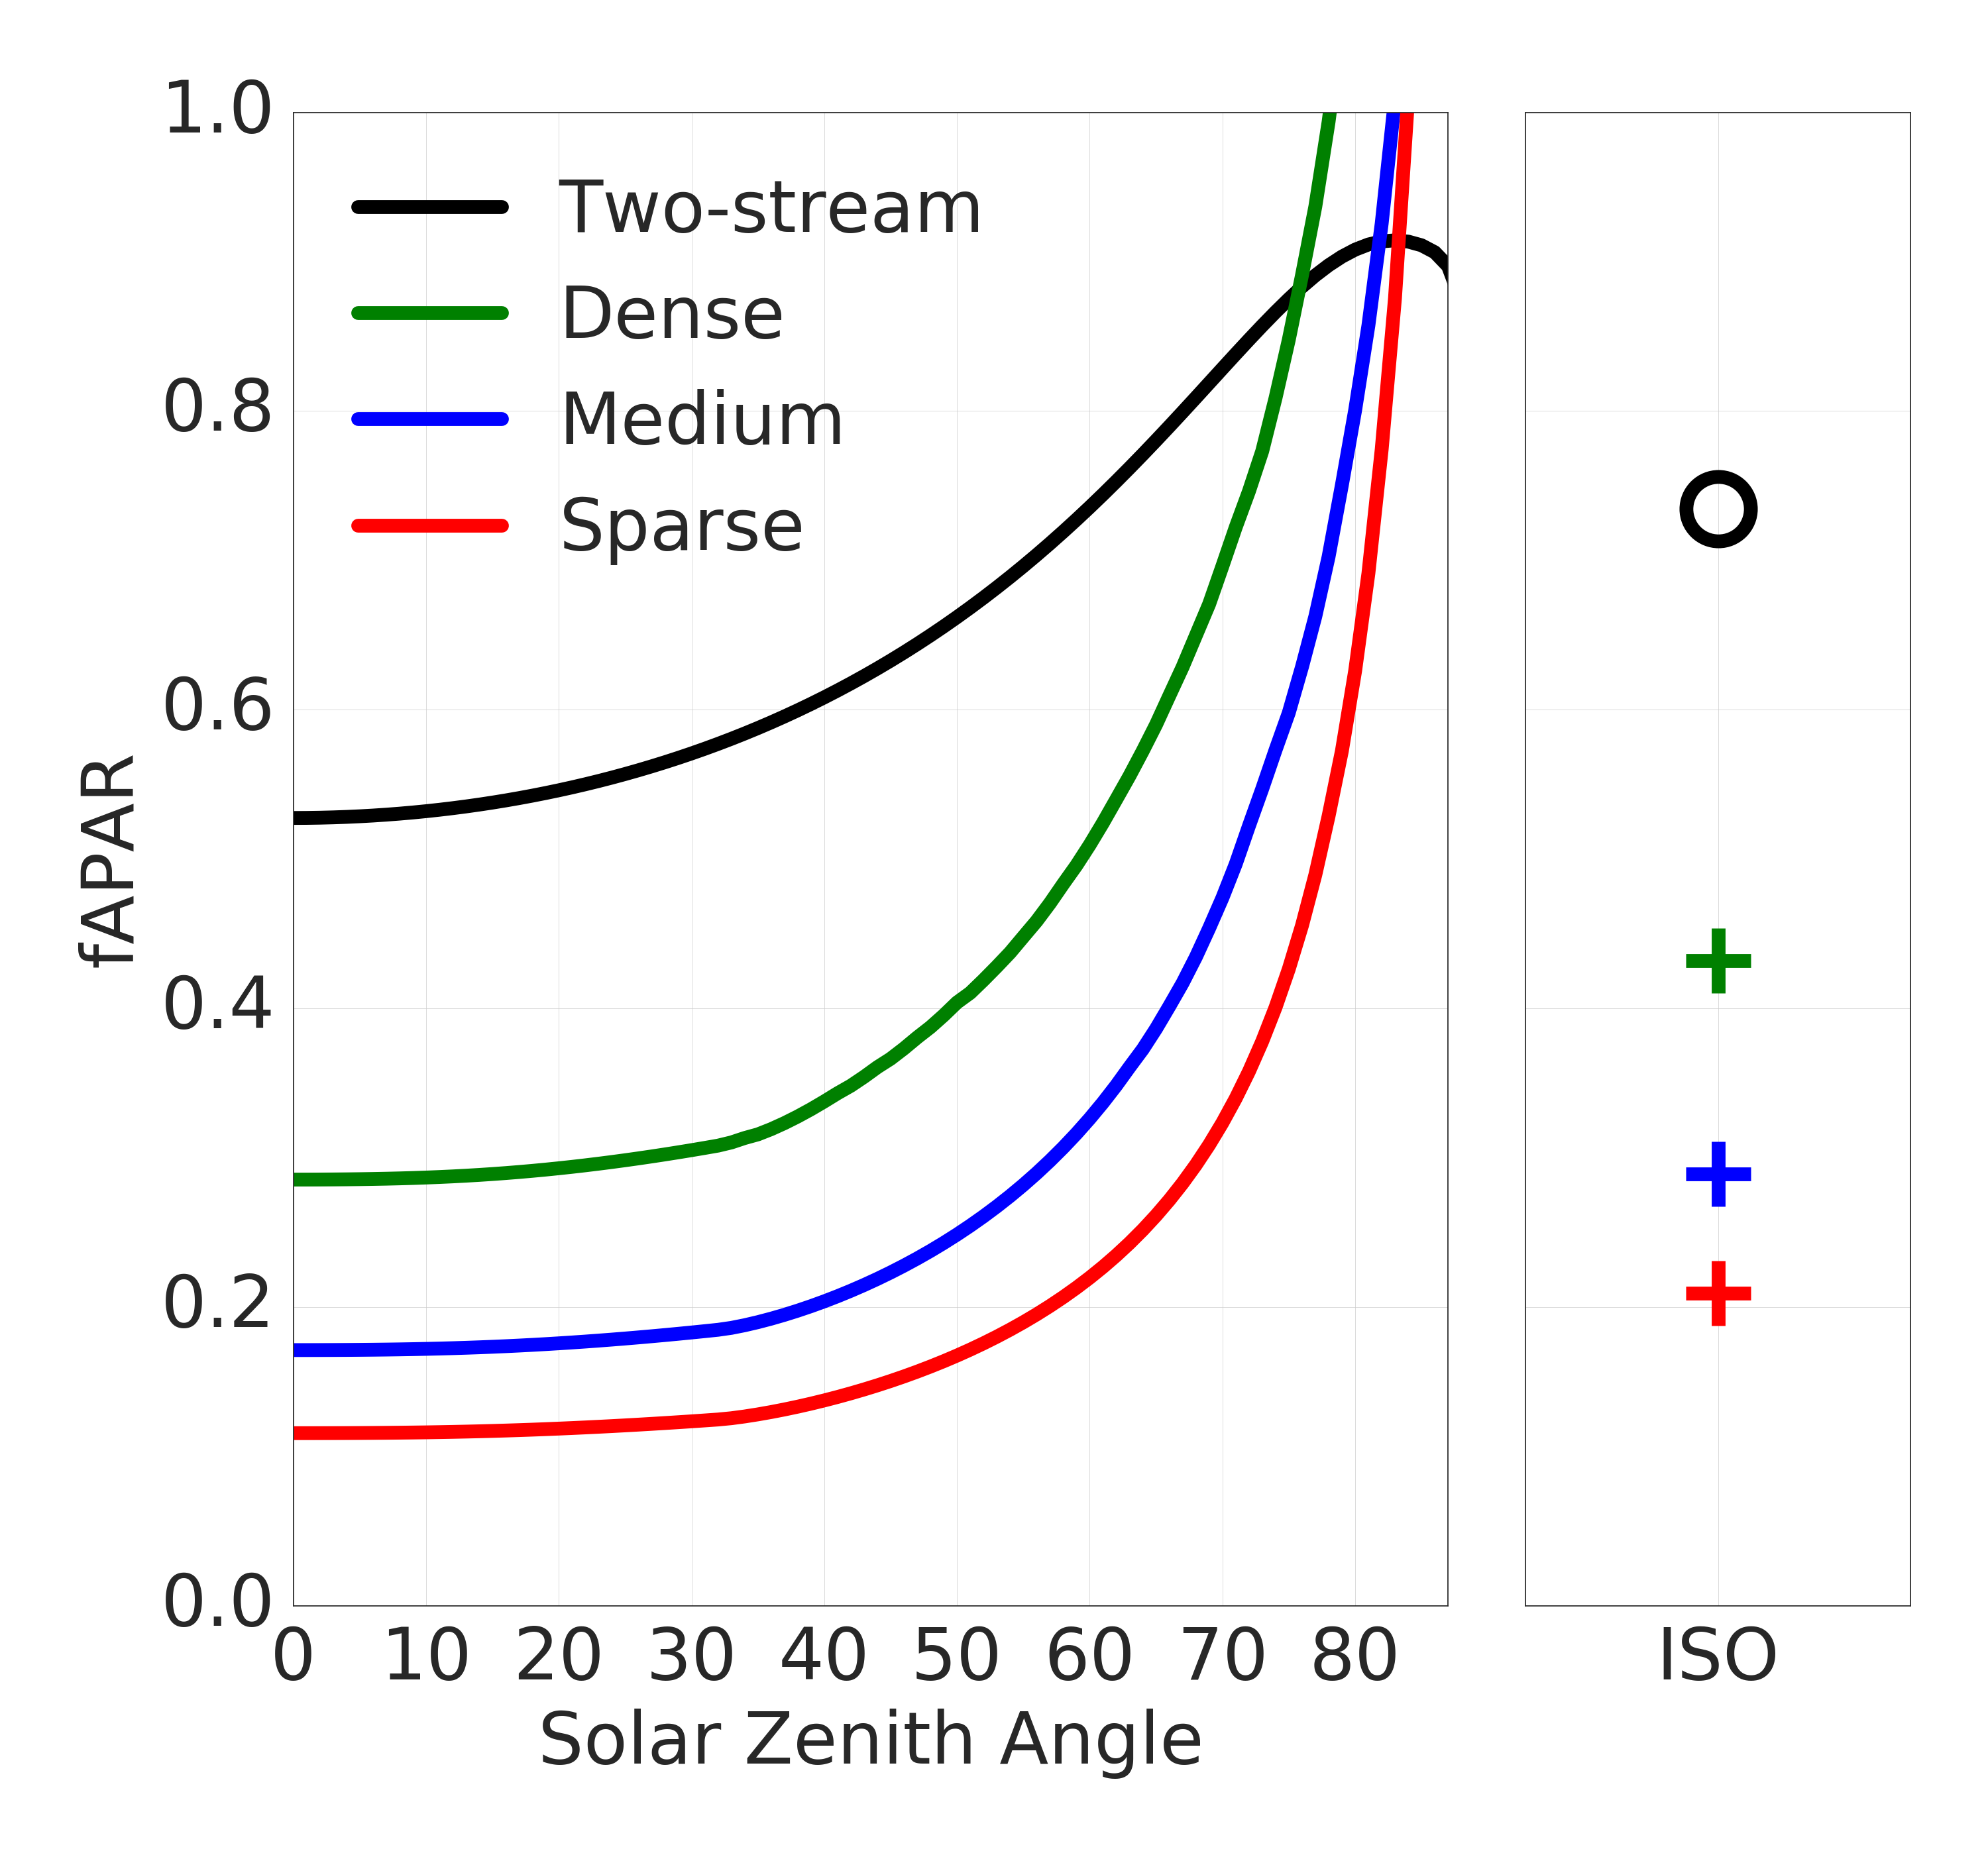
\includegraphics[width=0.5\textwidth]{/home/mn811042/Thesis/chapter4/figures/Sec_4.1/fapar_test.png}}
\subfloat[albedo PAR]{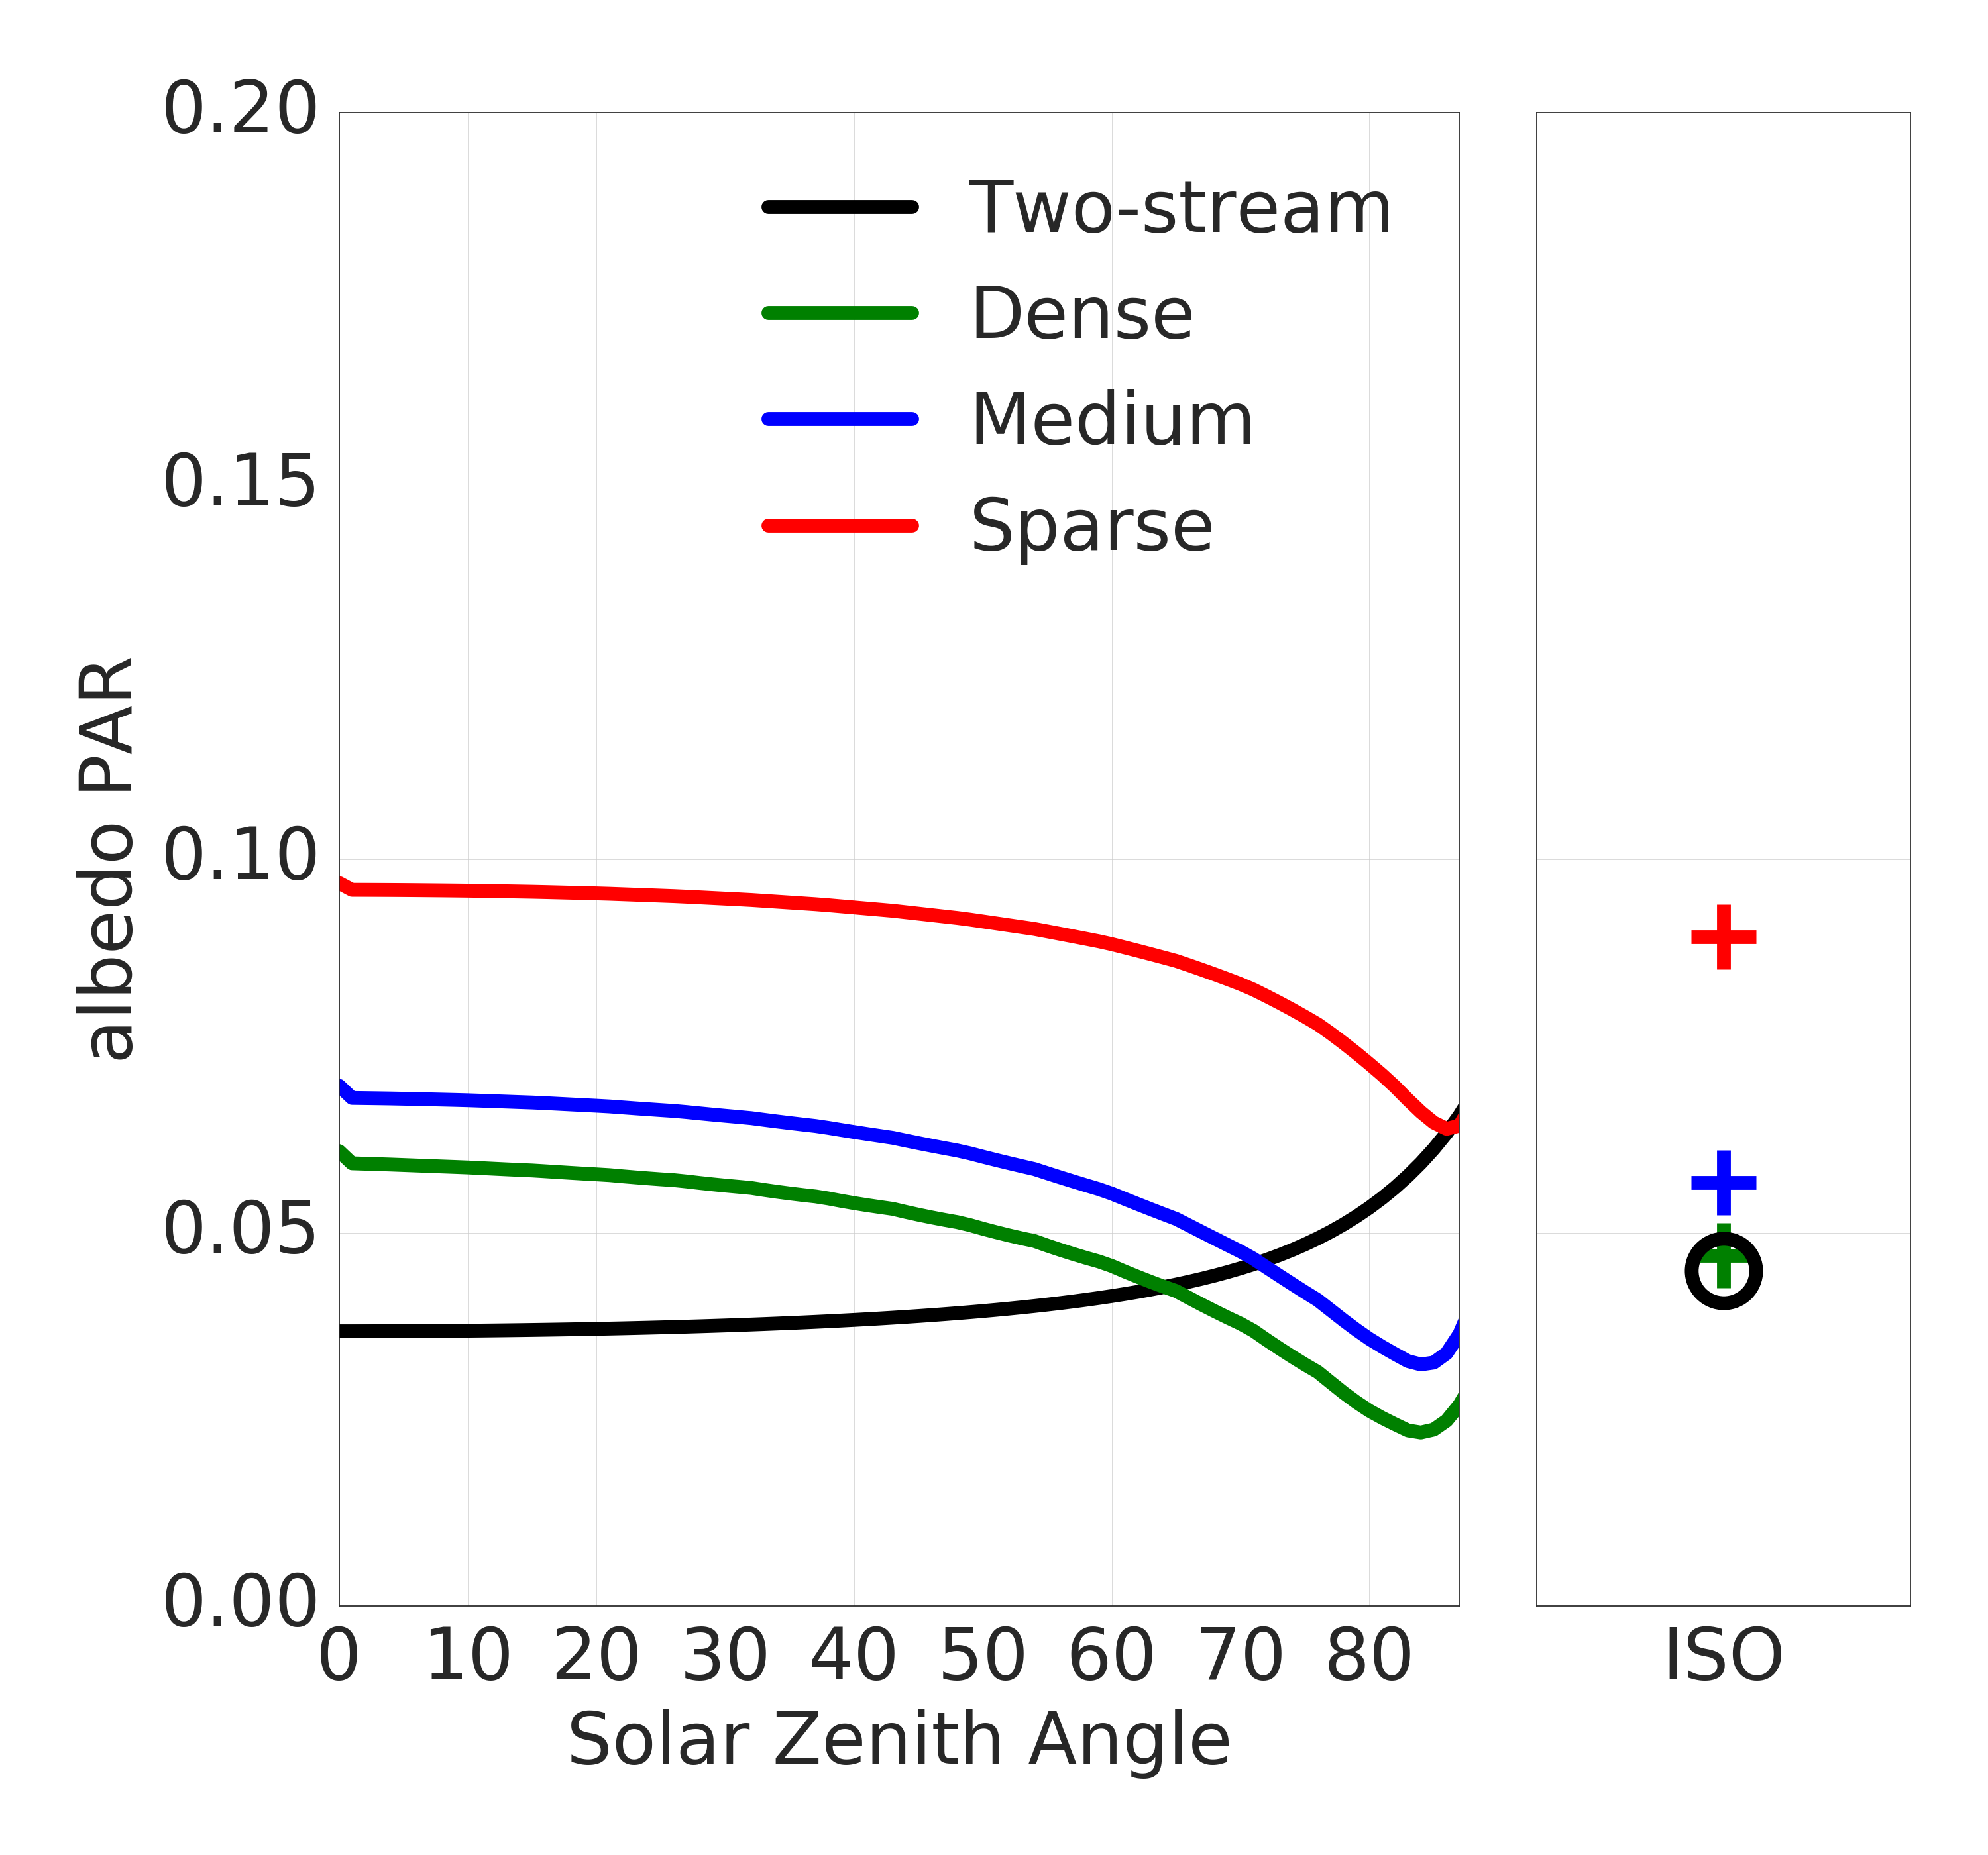
\includegraphics[width=0.5\textwidth]{/home/mn811042/Thesis/chapter4/figures/Sec_4.1/albpar_test.png}}
\end{tabular}

%\begin{tabular}{ll}
%\subfloat[fANIR]{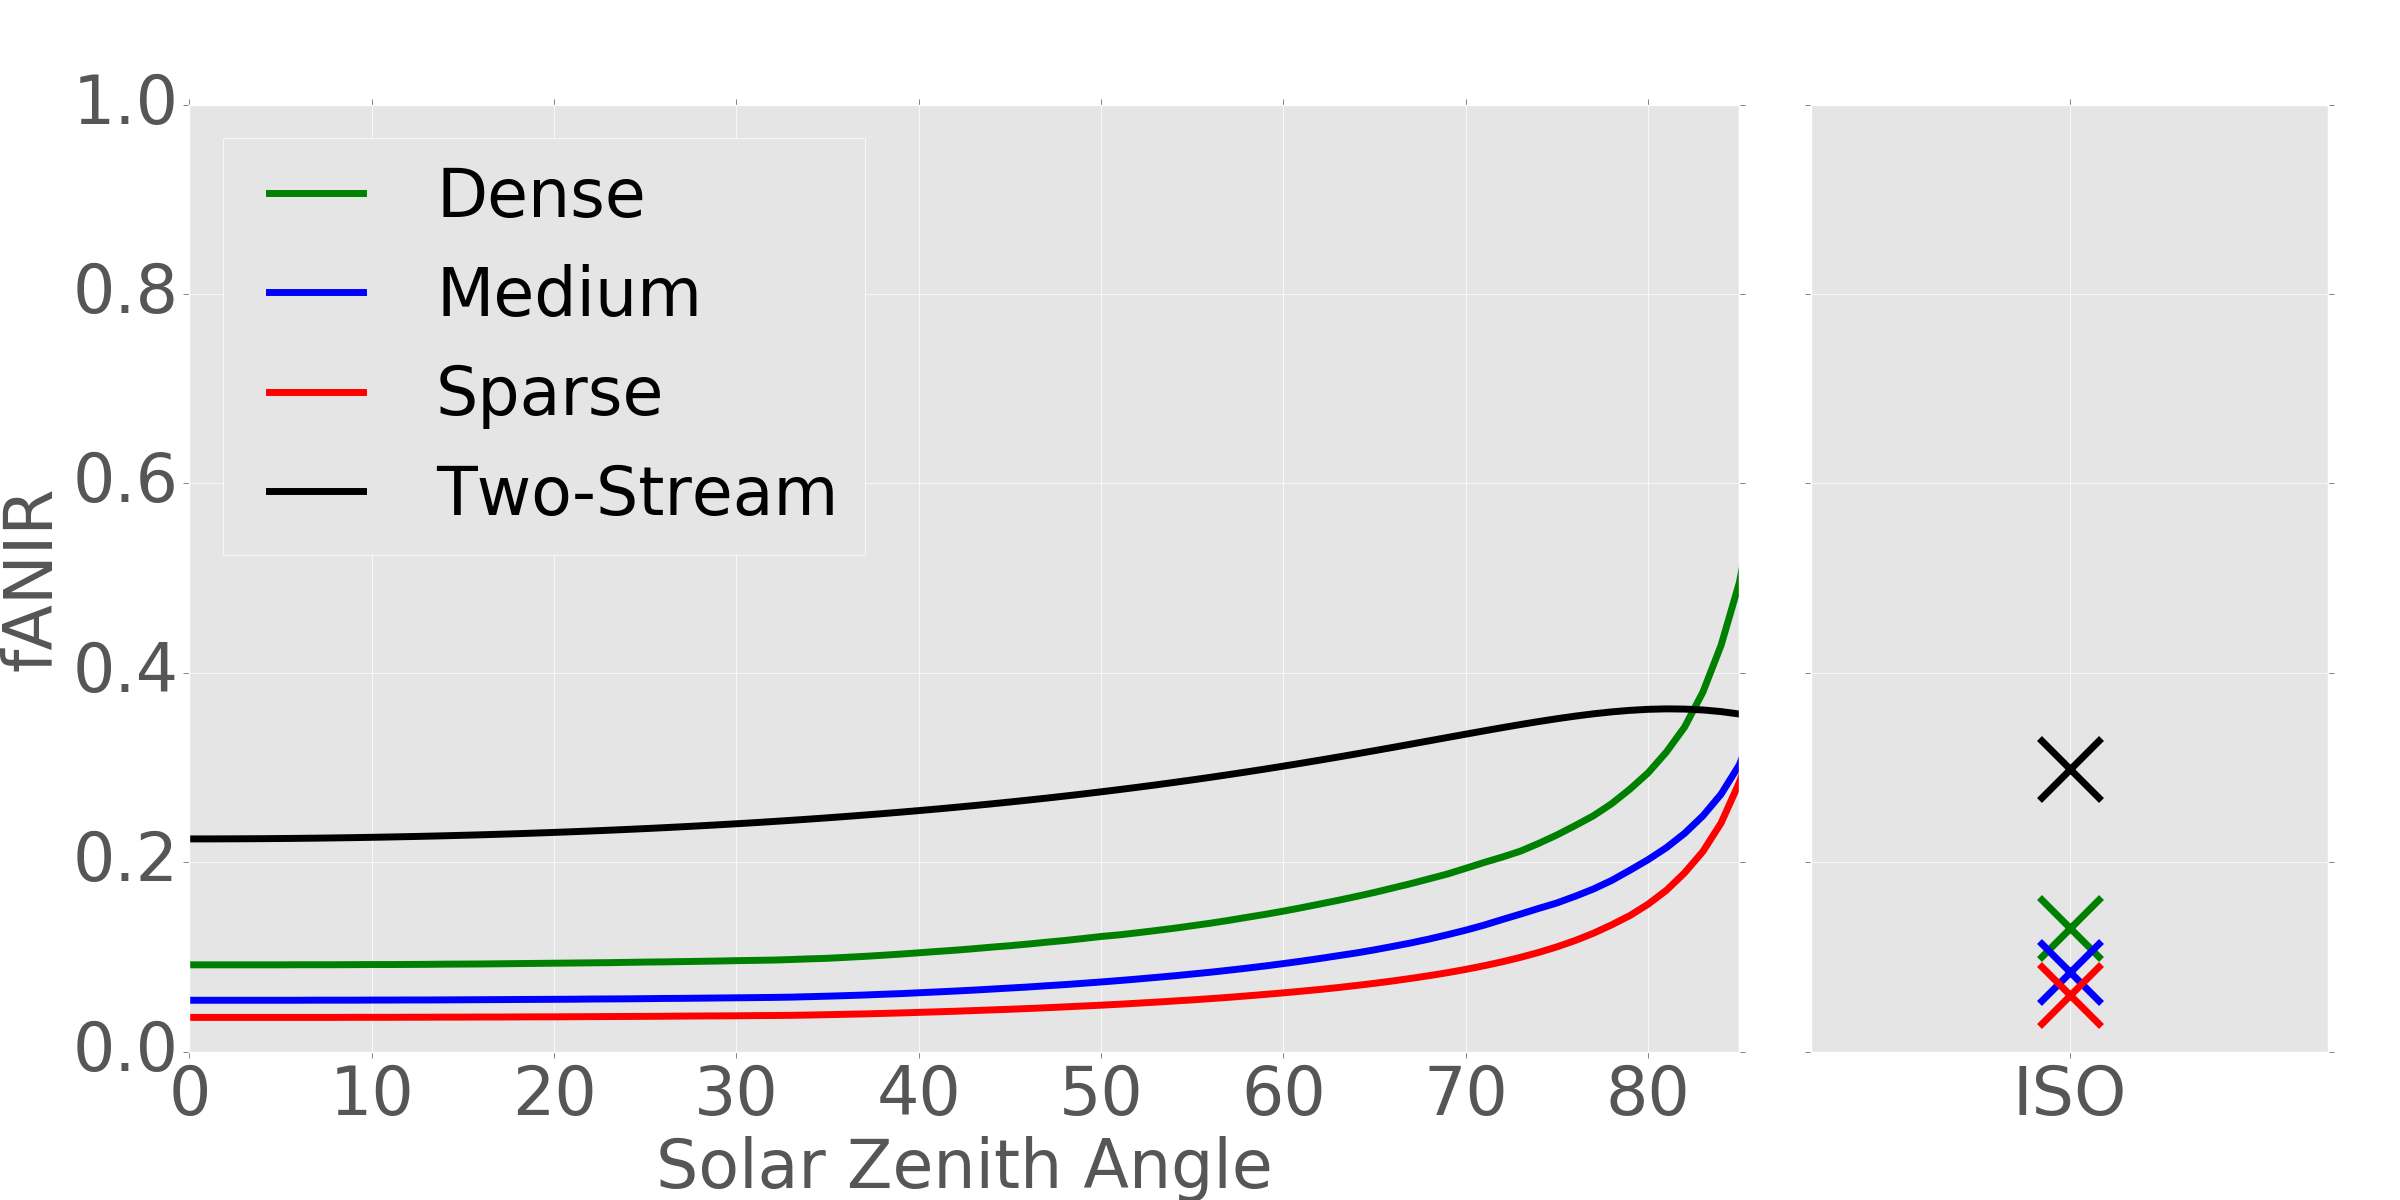
\includegraphics[width=0.5\textwidth]{/home/mn811042/Thesis/chapter4/figures/Sec_4.1/fanir_sza_lai_150_2.png}}
%\subfloat[albedo NIR]{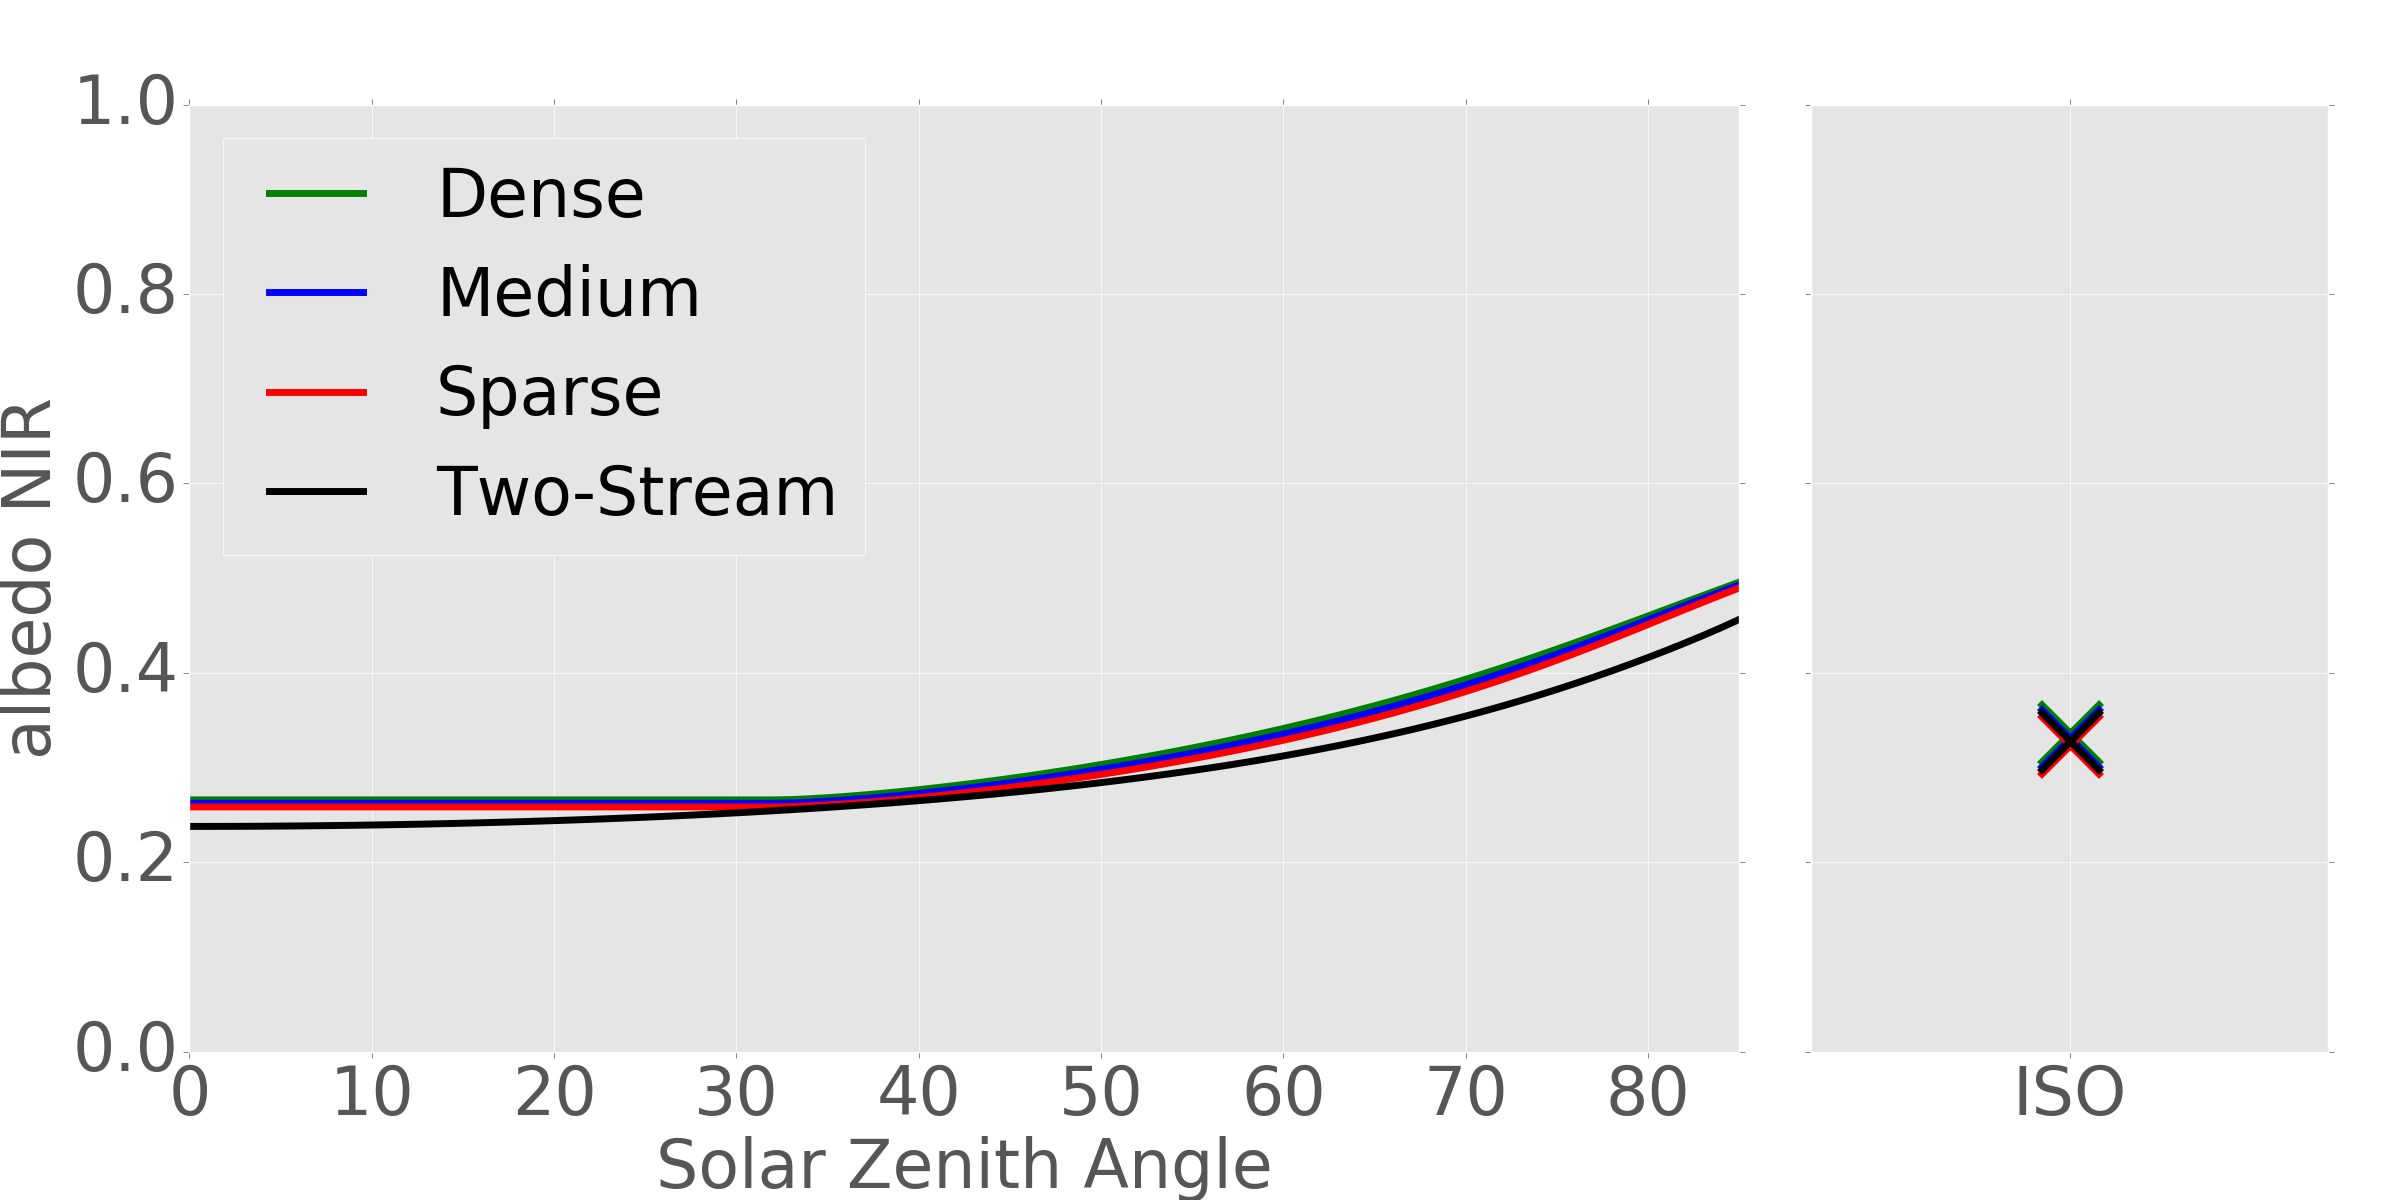
\includegraphics[width=0.5\textwidth]{/home/mn811042/Thesis/chapter4/figures/Sec_4.1/albnir_sza_lai_150_2.png}}
%\end{tabular}

\caption{Fraction of absorbed and reflected PAR (fAPAR and albedo PAR) respectively, calculated with the two-stream approach, and other two 3D radiative transfer models a) MAESPA for absorption; and b) GORT for reflectance, over three different vegetation canopy densities with same total scene LAI (1.5 m$^2$.m$^{-2}$).} 
\label{f:ts_maespa}
\end{figure}

Figure~\ref{f:ts_maespa} shows the zenith profile of fAPAR and albedo PAR from the two-stream approach, for three different canopy structures with same scene LAI. On the right hand side of each plot, with the symbol ISO (isotropic), it is represented the totally diffuse radiation case. In terms of absorbed PAR, the two-stream approach overestimates all the 3D scenarios for both types of illumination conditions, i.e., direct and diffuse. The dense scene has the closest values for PAR absorption with an average bias of -0.18. The bias between these two different models decreases with canopy density. For the medium case the bias is -0.35, and the sparse case presents the largest disagreement between the models, with an average bias of -0.44. The results indicate that for a scene with same total LAI but different structural arrangements, the overestimation of the two-stream approach can be as high as 44\% in PAR absorption. Almost half of the absorbed radiation in the PAR spectral region is in disagreement between the 1D and the 3D radiative transfer models used in this experiment, when the vegetation canopy is sparse.

%The results also highlight for the fact that the PAR spectral region is more than twice sensitive to canopy structure than the NIR spectral region. For all the evaluated cases the amount of absorbed radiation increases with solar zenith angle, as predicted by the radiative transfer theory, and so the Pearson coefficient is greater than 0.85 for all evaluated curves.

By contrast to canopy absorption, canopy reflectance is underestimated by the two-stream approach in comparison to GORT until a Sun zenith angle of approximately 60$^{\circ}$ for the the dense case, 70$^{\circ}$ for the the medium case, and over the whole zenith profile for the sparse case. The average bias of albedo PAR is up to 0.049 in the sparse case, which represents the same order of magnitude of the total averaged albedo PAR generated by the two-stream approach. The bias, correlation coefficients, and RMSEs between the two-stream approach, and the other two 3D radiative transfer models are summarised in Table~\ref{tab:statistical_lai}.

\begin{table}
\caption{Bias, correlation coefficient ($r$), and RMSE for model outputs between the two-stream approach and the MAESPA model for absorption, and between the two-stream and the GORT model for reflectance in the PAR spectral region (400 - 700 nm).}
 \begin{tabular*}{\textwidth}{ @{\extracolsep{\fill}} *{5}{l}}
\hline
\hline   
&  & Dense & Medium & Sparse\\
 \hline
\multirow{3}{*}{fAPAR} 
                   & Bias    & -0.177 &  -0.349 & -0.439\\
                   & $r$     &  0.892 &   0.909 &  0.856\\
                   & RMSE    &  0.262 &   0.366 &  0.449\\

\hline
\multirow{3}{*}{albedo PAR} 
                   & Bias    & 0.008  &  0.018 & 0.049\\
                   & $r$     & -0.977 & -0.981 & -0.998\\
                   & RMSE    & 0.018  & 0.024  & 0.051\\
% MAESPA
%                   & Bias    & 0.006 & 0.008 & 0.011\\
%                   & Pearson & 0.997 & 0.998 & 0.998\\
%                   & RMSE    & 0.006 & 0.008 & 0.011\\
%\hline
%\multirow{3}{*}{fANIR} 
%                   & Bias    & -0.134 & -0.186 & -0.212\\
%                   & Pearson &  0.892 &  0.909 &  0.856\\
%                   & RMSE    &  0.138 &  0.187 &  0.213\\
%\hline
%\multirow{3}{*}{albedo NIR} 
%                   & Bias    & 0.025 &  0.021 & 0.016\\
%                   & Pearson & 0.995 &  0.995 & 0.995\\
%                   & RMSE    & 0.027 &  0.023 & 0.019\\
\hline
\hline
 \end{tabular*}
\label{tab:statistical_lai}
\end{table}

This simple experiment performed with three different radiative transfer models indicates that using scene LAI alone is not sufficient to take into account differences in vegetation canopy structure, in order to calculate PAR radiative partitioning into the absorbed or reflected components. It also shows that the diffuse incident light is also impacted by vegetation structure, with overestimation caused by the two-stream approach regarding absorption, and underestimation for reflectance. Aligned with findings from other studies \citep{Yang2001,Widlowski2011,loew2014}, the results showed in this section used two suitable 3D radiative transfer models to consider the impacts of different canopy structures on PAR partitioning, and it raised limitations caused by the use of the two-stream approach on the correct estimation of absorbed, and reflected PAR, over spatially heterogeneous vegetation canopies.

Based on the results presented in this section, it is important to explore mechanisms of making the shortwave radiation partitioning calculated by the two-stream approximation behaves more like complex 3D radiative transfer models in the presence of architectural heterogeneity of the land surface, without losing its original efficiency.
%,so it could be applied over larger areas, for longer periods of time.

\section{Evaluating vegetation structural effects in the two-stream scheme: direct transmissivity}\label{section:parameterisations}

Previous studies \citep{Nilson1971,Wang1990} have shown, with observations \citep{Kucharik1999,Yang2001,yang2003,Jonckheere2004} and detailed modelling approaches \citep{Ni-Meister2010,Widlowski2011}, that vegetation structure influences shortwave radiation partitioning \citep{pinty2006,Chen2008}, and other land surface related processes \citep{Kobayashi2012,loew2014}.

For most natural woody vegetation, the spatial distribution of individual tree crowns creates clear spaces, whereas beam radiation propagates without interaction with vegetation elements, and so, the two-stream scheme results in large deviations from the actual amounts of absorbed, and reflected shortwave radiation.
%\citep{Ni-Meister2010,Kobayashi2012,loew2014}.

For detailed computation of 3D shortwave radiation fields within heterogeneous vegetation canopies, there are a number of more complex radiative transfer models; for example, the geometrical optical approach, where mixtures of individual trees and multiple scattering with foliage are treated within tree crowns, following an average distribution dependent on tree density, as in the GORT model \citep{Li1995}. Another commonly used approach is to treat heterogeneous vegetation canopies based on the description of each individual tree crowns, e.g. in MAESTRA/MAESPA \citep{Wang1990,Duursma2012}, among other more complex approaches, as the 3D Monte Carlo ray-tracing, as in the raytran model, used as reference in the RAMI4PILPS experiment. However, these models cannot be directly used in GCMs due to their computational demand \citep{Yang2001}, and the high number of required vegetation structural parameters \citep{loew2014}. 

Even though time efficient 1D radiative transfer models are still preferably used in numerical weather prediction models, or global climate models, mainly because of their simplicity, speed, and suitability for running over large areas, the use of effective radiative state variables to express the properties of 3D heterogeneous vegetation canopy structure makes a simpler model to analogously simulate the shortwave radiation partitioning of more complex 3D models \citep{Pinty2004,pinty2006}.

This type of state variable was first described as a `clumping index' by \citet{Nilson1971}, and it was associated with the heterogeneous nature of the vegetation canopy volume, often used at the tree resolution \citep{Norman1974,chen1992,Chen1996}. This variables were revisited later on by other authors \citep{Pinty2004,pinty2006}, who used the same scientific proposition to account for vegetation canopy structural heterogeneity of different radiative turbid media but at the stand scale, specially in association with new satellite derived products.

These clumping indices account for all phyto and woody elements composing the vegetation canopy. They were designed to work as a modulator of the vegetation canopy optical depth, in order to address vegetation heterogeneity. The clumping indices are often smaller than unit, which means that, in the presence of gaps structure decreases the total optical depth of a vegetation canopy. Oppositely, if the clumping index is greater than unit, it is often an indication of specific structural canopy conditions associated with significant amounts of woody elements \citep{pinty2006}.

Other authors \citep{Kucharik1999,Ni-Meister2010} attempted to formulate simplified modelling approaches to resolve vegetation clumping at several levels of organisation, from shoot to stand scales, in order to address the major differences in shortwave radiation partitioning between 1D and 3D radiative transfer schemes over non-homogeneous forest canopies based on semi-empirical formulations derived from direct transmissivity observations, or more complex radiative transfer models.

The next subsections describe and evaluate 4 different clumping indices to address vegetation heterogeneity in the modified version of the two-stream scheme. Evaluations are performed against a benchmarking exercise of radiative transfer in vegetation canopies, the RAMI4PILPS \citep{Widlowski2011}. Also, two other 3D radiative transfer models, MAESPA and GORT, already used previously are added into the evaluations, in order to determine their abilities and limitations over different spectral, and structural properties. Finally, a parameterisation scheme based on the proportion of vegetation cover, commonly used in LSMs to account for vegetation heterogeneity on a grid cell, is compared with the other approaches as well, in order to evaluated how appropriately LSMs treat shortwave radiation partitioning in the presence of vegetation structure.

\subsection{The RAMI4PILPS scenes}
The RAMI4PILPS experiment \citep{Widlowski2011} was designed to evaluate the accuracy and consistency of shortwave radiative transfer formulations, as used in LSMs by evaluating different models against the extensively verified 3D Monte Carlo ray-tracing model, raytran \citep{Govaerts1995}.

The ray-tracing code used in the RAMI4PILPS experiment allows the explicit representation of radiation transfer in arbitrarily complex scenes \citep{Govaerts1998} by implementing a Monte Carlo approach, where the fate of millions of individual rays are followed as they travel through the computer simulated scene.

In this chapter, the RAMI4PILPS heterogeneous canopy case is used, where tree crowns were approximated by woodless spheres in an open forest canopy scene. Details of the RAMI4PILPS experiments used in this study are summarised in Table~\ref{tab:RAMI4PILPS}; and a graphic representation of the experiment setups can be found in Figure~\ref{fig:rami}, while further details of the RAMI4PILPS experiments can be found in \citet{Widlowski2011}.

For each canopy density, simulations for different leaf area index, and different soil brightness are performed, assuming direct insulation for three different Sun zenith angles (27.5$^{\circ}$, 60.0$^{\circ}$, and 83.5$^{\circ}$), as well as isotropic illumination conditions (ISO), i.e., when global incident radiation is totally diffuse.

\begin{figure}
\centering
\begin{tabular}{lll}
\subfloat[Sparse Canopy]{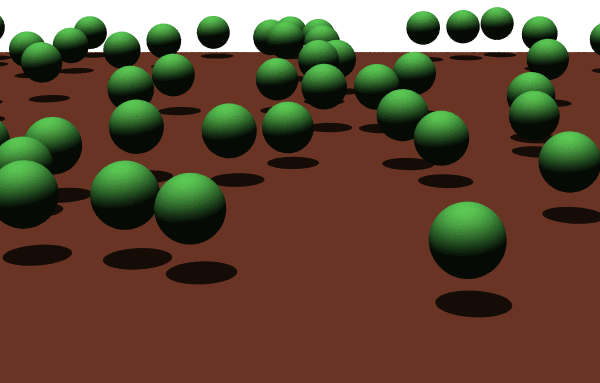
\includegraphics[width=0.33\textwidth]{/home/mn811042/Thesis/chapter4/figures/rami_lai_050.png}}
\subfloat[Medium Canopy]{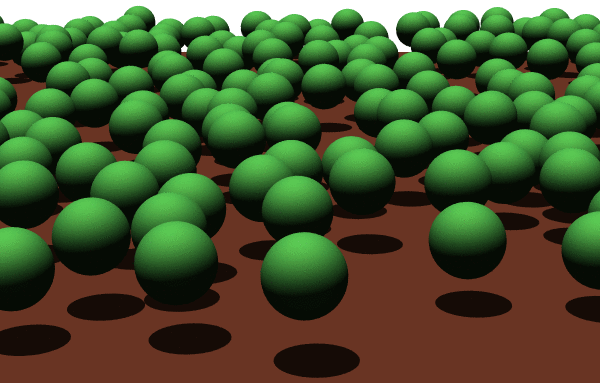
\includegraphics[width=0.33\textwidth]{/home/mn811042/Thesis/chapter4/figures/rami_lai_150.png}}
\subfloat[Dense Canopy]{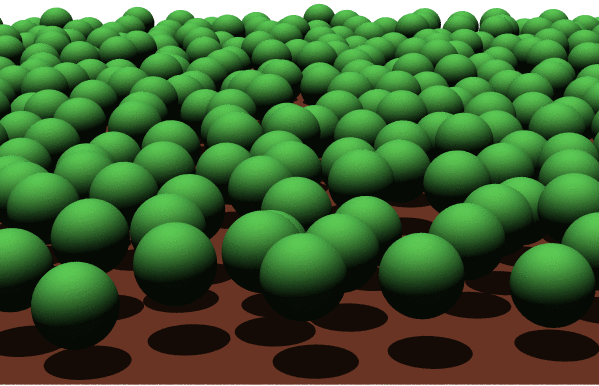
\includegraphics[width=0.33\textwidth]{/home/mn811042/Thesis/chapter4/figures/rami_lai_250.png}}
\end{tabular}
\caption{Graphical representation of the open forest canopy environments used in RAMI4PILPS. The images represent three different canopy structures (taken from \citet{Widlowski2011}).} 
\label{fig:rami}
\end{figure}

\begin{threeparttable}
\centering
\caption{Summary of variables defining structurally heterogeneous scenes (see \citet{Widlowski2011} for details). Different soil albedos are defined as BLK = black, MED = medium, and SNW = snow.}
%\begin{tabular*}{\textwidth}{ l@{\extracolsep{\fill}}*{4}{c}}
\begin{tabular}{l{0.25\textwidth} l{0.75\textwidth}}
%\begin{tabular}{\textwidth}{|p{\textwidth/4}|p{\textwidth/4}|p{\textwidth/4}|p{\textwidth/4}|}
%\begin{tabular*}
     \hline
     \hline
\textbf{Variable Identification}   & \textbf{Values (Units)}\\
\noalign{\smallskip}\hline
Leaf Area Index/ canopy	                & 0.50$^S$, 1.50$^M$ and 2.50$^D$ (m$^2$.m$^{-2}$)\\
Leaf Area Index/ sphere	                & 5.0$^S$, 5.0$^M$ and 5.0$^D$  (m$^2$.m$^{-2}$)\\
1 - $P_{gap} (\theta = 0^{\circ})$      & 0.09$^S$, 0.26$^M$ and 0.43$^D$\\
Tree density                            & 12.80$^S$, 38.24$^M$ and 63.68$^D$ (trees/hectare)\\
Maximum canopy height                   & 16 m\\
Minimum sphere centre height	        & 7 m\\
Maximum sphere centre height	        & 11 m\\
$\alpha_{soil}$,PAR / $\alpha_{soil}$,NIR	& BLK: 0.00/0.00; MED: 0.12/0.21; SNW: 0.96/0.56\\
Soil scattering law	                & Lambertian\\
$\rho_{leaf}$,PAR / $\rho_{leaf}$,NIR   & 0.0735/0.3912\\
$\tau_{leaf}$,PAR / $\tau_{leaf}$,NIR   & 0.0566/0.4146\\
Leaf scattering law                     & Bi-Lambertian\\
Sun zenith angle	                & 27.5$^{\circ}$/60.0$^{\circ}$/83.5$^{\circ}$/Isotropic(ISO)\\
Scatterer Normal Distribution           & Spherical\\
Woody area index                        & 0.0 (m$^2$.m$^{-2}$)\\
\hline
\hline%\noalign{\bigskip}
%\end{tabular*}
\end{tabular}
\begin{tablenotes}
      \small
      \item $^S$Sparse vegetation. $^M$Medium vegetation. $^D$Dense vegetation. 
\end{tablenotes}
\label{tab:RAMI4PILPS}
\end{threeparttable}
\bigskip

\subsection{The clumping index of Nilson (1971)}

To consider the non-random spatial distribution of leaves, \citet{Nilson1971} first proposed a Markov-chain model introducing an additional quantity, $\Omega$, into Eq.~\ref{equation:pgapnilson}:
\begin{equation}
P_{gap}(\theta) = \exp{(\frac{-G(\theta)  LAI  \Omega}{cos(\theta)})}
\label{equation:pgapnilson}
\end{equation}
\noindent where P$_{gap}$($\theta$) is the direct transmissivity, G($\theta$) is the leaf angle distribution function \citep{Ross1981}, LAI is the total scene LAI, $\theta$ is the Sun zenith angle, $\Omega$ is the clumping index.

The complete zenith profile of P$_{gap}$($\theta$) was then calculated by the MAESPA model as 1 - fAPAR for a black canopy, i.e., with leaf reflectance and transmittance equal zero, as well as soil albedo. As MAESPA is considered to be a robust tool to calculate absorbed PAR, by appling the Beer\textquotesingle s law to a black body, in this case the different canopy densities described by the RAMI4PILPS scenes, if the light is not absorbed by the vegetation canopy, the light is then transmitted through it. The clumping index was derived as the adjusted angular coefficient of the inverted Eq.~\ref{equation:pgapnilson}, and the values are summarised in Table~\ref{tab:niclumpparameters}.

\begin{threeparttable}
\centering
\caption{Summary of the clumping index parameters through the methodology of \citet{Nilson1971}.}
\begin{tabular*}{\textwidth}{ l@{\extracolsep{\fill}}*{4}{c}}
%\begin{tabular}{{0.33\textwidth} {0.33\textwidth} {0.33\textwidth}}
%\begin{tabular}{\textwidth}{|p{\textwidth/4}|p{\textwidth/4}|p{\textwidth/4}|p{\textwidth/4}|}
%\begin{tabular*}
     \hline
     \hline
\textbf{Variable}   & \textbf{$\Omega$}\\
\noalign{\smallskip}\hline
Sparse & 0.362 \\
Medium & 0.402 \\
Dense  & 0.470 \\
\hline
\hline%\noalign{\bigskip}
%\end{tabular*}
\end{tabular*}
\label{tab:niclumpparameters}
\end{threeparttable}
\bigskip

\subsection{The clumping index of Kucharik et al. (1999)}

In this method, two key quantities are needed: (i) the fraction of ground area covered by the horizontal projection of crown envelopes (Veg$_{frac}$) (from nadir view), which is a function of the typical tree crown diameter ($D$), and tree stem spacing ($\lambda$), or stem density, within a study plot; and (ii) an estimate of crown porosity ($\Phi$); this quantity is related to foliage density and defined as the gap fraction within crown envelopes divided by Veg$_{frac}$.

To characterise the angular dependence of $\Omega(\theta)$, a minimum value of $\Omega(\theta)$ was determined at $\theta$ = 0$^{\circ}$ and a value of $\Omega(\theta)$ was needed at $\theta$ = 90$^{\circ}$. Because it was assumed that $\Omega(\theta)$ reaches its maximum value at $\theta$ = 90$^{\circ}$, \citet{Kucharik1999} refer to this value as the maximum possible element clumping index, $\Omega_{max}$, and defines it as:
\begin{equation}
\Omega_{max} = \Big(\frac{ND}{\sqrt{A}}\Big)^{0.7}
\label{equation:clumpmax}
\end{equation}
\noindent where $N$ is number of stems within ground area $A$, and $D$ is crown diameter. If $ND/\sqrt{A} > 1$, then the value of $\Omega_{max} = 1$. The angular dependence of $\Omega(\theta)$ was defined by \citet{Kucharik1999} following the equation: 
\begin{equation}
\Omega = \Omega(\theta) = \frac{\Omega_{max}}{[1 + b\exp(-k(\theta)^p)]}
\label{equation:clumptheta}
\end{equation}
\noindent where $k$ is constant (usually $k$ = 2.2), $\theta$ is zenith angle expressed in radians, and $b$ is solved from a rearrangement of Eq.~\ref{equation:clumptheta} using a known value of $\Omega(\theta)$ (e.g., $\theta$ = 0$^{\circ}$). A quantitative comparison of results produced using Eq.~\ref{equation:clumptheta} with the best-fit curves suggested that a value for $p$ can be approximated by an equation on the form:
\begin{equation}
p = -0.461\chi + 3.8
\label{equation:pchi}
\end{equation}
\noindent where $\chi$ is the ratio of crown depth to crown diameter. Generally, if $\chi$ is $\leq$ 1.0, $p$ = 3.34. 

This set of semi-empirical equations was used to estimate clumping index for three different canopy sets as in RAMI4PILPS (Table~\ref{tab:RAMI4PILPS}). The results calculated by Eq.~\ref{equation:clumptheta} are presented by dotted lines in Figure~\ref{f:ci_comparisons}, and summarised in Table~\ref{tab:kucharikclumpparameters}.

\begin{threeparttable}
\centering
\caption{Summary of the clumping index parameters of \citet{Kucharik1999}.}
\begin{tabular*}{\textwidth}{ l@{\extracolsep{\fill}}*{4}{c}}
%\begin{tabular}{{0.33\textwidth} {0.33\textwidth} {0.33\textwidth}}
%\begin{tabular}{\textwidth}{|p{\textwidth/4}|p{\textwidth/4}|p{\textwidth/4}|p{\textwidth/4}|}
%\begin{tabular*}
     \hline
     \hline
\textbf{Variable}   & \textbf{$\Omega_{max}$} & \textbf{$b$}\\
\noalign{\smallskip}\hline
Sparse & 0.33 & 1.44\\
Medium & 0.70 & 14.03\\
Dense  & 1.00 & 3.48\\
\hline
\hline%\noalign{\bigskip}
%\end{tabular*}
\end{tabular*}
\label{tab:kucharikclumpparameters}
\end{threeparttable}
\bigskip

%The range of clumping index obtained by this work was from approximately 0.2, for minimum Sun zenith angle (i.e. $\theta = 0^{\circ}$), with convergence to 1, for maximum Sun zenith angle (i.e. $\theta = 90^{\circ}$), for sparse and dense canopies, while the convergence in high solar zenith angles ($\theta > 70^{\circ}$) for the medium canopy was approximately 0.7, starting with very small $\Omega(\theta) \approx$ 0.0.

\subsection{The clumping index of Pinty et al. (2006)}\label{section:pintyscheme}

Among other parameterisation schemes, the one proposed by \citet{pinty2006} presents a relatively self-sufficiency, because it does not require any previous knowledge about vegetation structure, and because of that, it can be applied to any vegetation canopy. The values of the effective variables can be estimated by inverting the results from the two-stream approach against the results obtained by a 3D radiative transfer model model \citep{pinty2006}.

Previous studies have reported the dependency of clumping index on zenith angle variations \citep{Andrieu1993,Chen1996,Kucharik1999,Leblanc2005,Ryu2010}. This dependency remains rather smooth, and limited \citep{Chen1997a,Chen1997}, and it was written by \citet{pinty2006} following an approximated linear relationship:
\begin{equation}
\Omega = \zeta(\mu) \approx a + b \cdot (1 - \mu)
\label{equation:structurefactor}
\end{equation}
\noindent where $\mu$ is the cosine of $\theta$, $a = \zeta(\mu=1)$ is the parameter corresponding to an overhead Sun and $b$, the parameter that includes the effects of different Sun geometries. In the particular case of an overhead Sun ($\theta$ = 0$^{\circ}$), $a$ is described in \citet{pinty2006} as being equal to:
 \begin{equation}
\zeta(\mu=1) = -\ln{(1 - F_c)}\frac{2}{LAI}
\label{equation:structurefactora}
\end{equation}
\noindent where $F_c$ is the true vegetation cover (accounting for within and between crown gaps). Both parameters are used to account for vegetation canopy heterogeneity, and they are used to modulate the shortwave radiation path length. In this exercise, however, both parameters were freely minimised against the RAMI4PILPS reference values for PAR absorption and reflectance.

\bigskip
\noindent\textbf{Determing the structure factor parameters}
\bigskip

\noindent Both structure factor parameters, $a$ and $b$ in Eq.~\ref{equation:structurefactor}, were freely minimised against the RAMI4PILPS reference values without following a prescriptive equation. The structure factor parameters were obtained for each canopy structure through the inversion of the two-stream scheme against direct and diffuse, fAPAR and albedo PAR reference values from the RAMI4PILPS experiment. The Nelder-Mead minimisation method \citep{Nelder1964}, or `downhill simplex' was used in the inversion process.

To minimise the structure factor parameters in respect to canopy density, a minimum error evaluation was conducted varying $a$ and $b$ from 0.0 to 1.0 following the equation:
\begin{equation}
RMSE_{ab} = \sqrt{\frac{\sum_{n=1}^{N} (f_{Two-stream} - f_{MAESPA})^2}{N}}
\label{equation:rmseab}
\end{equation}
\noindent N = 85, $a$ = [0,1], $b$ = [0,1], and $f_{two-stream}$ is the fAPAR calculated with the two-stream radiative transfer scheme with the structure factor parameterisation for a combination of $a$\textquotesingle s and $b^$\textquotesingle s, and  $f_{MAESPA}$ is the fAPAR reference value calculated with the MAESPA model for different Sun zenith geometries, varying from 0$^{\circ}$ to 85$^{\circ}$. fAPAR values from MAESPA have been validated (Figure~\ref{f:szacomparisonfPAR}), and the model has been shown to be a valid tool to calculate PAR absorption for different vegetation canopies, as it strongly agreed with the RAMI4PILPS reference values, except over large soil albedos (SNW).

The results showed in Figure~\ref{f:rmsd_ts_maespa} are limited to the PAR spectrum, with an intermediate value of background albedo ($\alpha_{soil} = 0.12$). However, for all the evaluated cases, the combination of $a$ and $b$ that gives the minimum error between the 1D and the 3D cases, is not a single value but a combination of values, described by a certain area of minimum RMSE. This finding suggests that for a particular forest stand, there is not only a single combination of $a$\textquotesingle s and $b$\textquotesingle s but a number of combinations that modifies the radiative transfer calculations of the two-stream approach, and makes it matches the radiation partitioning of more complex 3D models. The elliptical shape of the minimum error area in Figure~\ref{f:rmsd_ts_maespa}, for all canopy densities, indicates that the range of minimum $a$\textquotesingle s is smaller than the range of possible $b$\textquotesingle s, which suggests a stronger effect of $a$ in comparison to $b$ on modulating the radiative fluxes calculated by the two-stream approach.

The sparse case, however, seems to be more closely sensitive to the parameters $a$ and $b$ together, as the ellipse that describes the minimum RMSE is inclined towards the y-axis. As canopy density increases, the sensitivity of $a$ starts to increase in relation to $b$, as it can be noticed by the larger error variation on the x-axis of $a$. This indicates that for denser canopies, $b$ has a reduced impact due to architectural effects on shortwave radiation partitioning, if compared to $a$.

\begin{figure}
\centering
\begin{tabular}{lll}
\subfloat[LAI = 0.5 m$^2$.m$^{-2}$]{\includegraphics[width=0.33\textwidth]{/home/mn811042/src/julesRT_struct_2/julesRT_struct/RMSE_JULESRT_v2_MAESPA_050.png}}
\subfloat[LAI = 1.5 m$^2$.m$^{-2}$]{\includegraphics[width=0.33\textwidth]{/home/mn811042/src/julesRT_struct_2/julesRT_struct/RMSE_JULESRT_v2_MAESPA_150.png}}
\subfloat[LAI = 2.5 m$^2$.m$^{-2}$]{\includegraphics[width=0.33\textwidth]{/home/mn811042/src/julesRT_struct_2/julesRT_struct/RMSE_JULESRT_v2_MAESPA_250.png}}
\end{tabular}
\caption{Root-Mean-Squared-Error for Two-Stream scheme with the structure factor parameterisation and MAESPA for three canopies densities (sparse, medium and dense).}
\label{f:rmsd_ts_maespa}
\end{figure}

The structure factor parameters obtained for each canopy density through the inversion of fAPAR and albedo PAR together, over three soil backgrounds at the same time are summarised in Table~\ref{tab:structureparameters}:

\begin{threeparttable}
\centering
\caption{Summary of the structure factor parameters minimised against the absorption and reflectance reference values for the PAR waveband.}
\begin{tabular*}{\textwidth}{ l@{\extracolsep{\fill}}*{4}{c}}
%\begin{tabular}{{0.33\textwidth} {0.33\textwidth} {0.33\textwidth}}
%\begin{tabular}{\textwidth}{|p{\textwidth/4}|p{\textwidth/4}|p{\textwidth/4}|p{\textwidth/4}|}
%\begin{tabular*}
     \hline
     \hline
\textbf{Variable}   & \textbf{$a$} & \textbf{$b$}\\
\noalign{\smallskip}\hline
Sparse & 0.344 & 0.096\\
Medium & 0.337 & 0.256\\
Dense  & 0.418 & 0.206\\
\hline
\hline%\noalign{\bigskip}
%\end{tabular*}
\end{tabular*}
\label{tab:structureparameters}
\end{threeparttable}
\bigskip

\subsection{The clumping index by Ni-Meister et al. (2010)}
Following the same attempt to derive a relationship for clumping index, \citet{Ni-Meister2010} developed an analytical prognostic expression based on stem density ($\lambda$), crown radius ($R$), and LAI. Only the equation used for spherical crowns is shown \citet{Li1988}. The analytical solution for the modified clumping index in Beer\textquotesingle s law is expressed as, 
\begin{equation}
\Omega = \gamma = \frac{3}{4\tau_0R}\Big(1 - \frac{1 - (2\tau_0R + 1)\exp(-2\tau_0R)}{2\tau_0^2R^2}\Big)
\label{equation:clumpNi}
\end{equation}
\noindent where $\tau_0r = 3 G LAI/ 4 \lambda \pi \cdot R^2$ for spherical crowns. 

The authors validated the analytical solutions for clumping index with the ones calculated by the full GORT model \citep{Li1995}, which was specifically developed to describe the effects of 3D canopy structure on the radiative partitioning, and to characterise the shortwave radiative partitioning in natural heterogeneous vegetation at the forest stand scale. This set of equations was used to estimate clumping index for three different canopy sets, as in RAMI4PILPS (Table~\ref{tab:RAMI4PILPS}), as well. The results calculated by Eq.~\ref{equation:clumpNi} are presented in Figure~\ref{f:ci_comparisons}. 

In the RAMI4PILPS experiment, canopy sets were defined with scene LAI increasing with tree density. The resulting clumping index calculated by the method described in this section was found to be constant for all the three canopy densities. That indicates that the clumping index of \citet{Ni-Meister2010} identifies structural differences in a very linked way with the scene LAI. Values for the three canopy densities as proposed in the RAMI4PILPS exercise are the same, and this particular clumping index formulation does not take into account differences in solar geometry.

\begin{threeparttable}
\centering
\caption{Summary of the clumping index parameters through \citet{Ni-Meister2010} methodology.}
\begin{tabular*}{\textwidth}{ l@{\extracolsep{\fill}}*{4}{c}}
%\begin{tabular}{{0.33\textwidth} {0.33\textwidth} {0.33\textwidth}}
%\begin{tabular}{\textwidth}{|p{\textwidth/4}|p{\textwidth/4}|p{\textwidth/4}|p{\textwidth/4}|}
%\begin{tabular*}
     \hline
     \hline
\textbf{Variable}   & \textbf{$\gamma$}\\
\noalign{\smallskip}\hline
Sparse & 0.349 \\
Medium & 0.349 \\
Dense  & 0.349 \\
\hline
\hline%\noalign{\bigskip}
%\end{tabular*}
\end{tabular*}
\label{tab:niclumpparameters}
\end{threeparttable}
\bigskip

\subsection{Comparing clumping indices}

Different ways to evaluate the performance of a specific radiative transfer scheme were proposed before, including comparisons against different sources of observed data, such as bidirectional reflectance \citep{North1996,Malenovsky2008}, transmittance measurements at stand scale in various levels \citep{Norman1983,Wang1990,Tournebize1995,Law2001a,Sinoquet2001}, and gap fraction measurements \citep{Cescatti1997,Kucharik1999,Yang2010}. However, the use of field data is often limited, and in order to eliminate uncertainties arising from an incomplete, or erroneous knowledge of structural, spectral, and illumination conditions related to canopy architectural characteristics, typically found in model comparisons with \textit{in situ} observations, model intercomparison exercises have been often used in research \citep{Pinty2001,Pinty2004,Widlowski2007,Widlowski2011,Widlowski2013}. This section focus specifically on an example of a model intercomparison.

Direct transmissivity was calculated following the P$_{gap}$ Eq.~\ref{equation:pgapnilson} for each one of the different clumping indices ($\Omega$\textquotesingle s) - $\Omega$ \citep{Nilson1971}, $\Omega_e(\theta)$ \citep{Kucharik1999}, $\zeta(\mu)$ \citep{pinty2006}, and $\gamma$ \citep{Ni-Meister2010} (Figure~\ref{f:ci_comparisons} right). The 1D case, or the Beer\textquotesingle s law, was also calculated following the same Eq.~\ref{equation:pgapnilson} with $\Omega$ = 1.0.

The 3D tree-based model, MAESPA, was used in the simulations of $P_{gap}(\theta)$ for the RAMI4PILPS scenes, and it was used as the reference model. $P_{gap}(\theta)$ was directly derived from MAESPA by setting a black canopy ($\rho_{leaf} = \tau_{leaf} = 0.0$) with different structures, and deriving it from fAPAR, as described below,
\begin{equation}
P_{gap}(\theta) = 1.0 - fAPAR(\theta)
\label{equation:pgap_black}
\end{equation}

To evaluate the differences between each one of the described parameterisations, the RMSE was calculated following Eq.~\ref{equation:rmse_pgap},
\begin{equation}
RMSE = \sqrt{\frac{\sum_{n=0}^{N} (P_{gap}(\theta)^{\Omega} - P_{gap}(\theta)^{MAESPA})^2}{N}}
\label{equation:rmse_pgap}
\end{equation}
\noindent where N = 85 because MAESPA presents numerical instability for very large Sun zenith angles (from 85$^{\circ}$ to 90$^{\circ}$).

\begin{figure}
\centering
\begin{tabular}{ll}
\subfloat[Sparse Canopy]{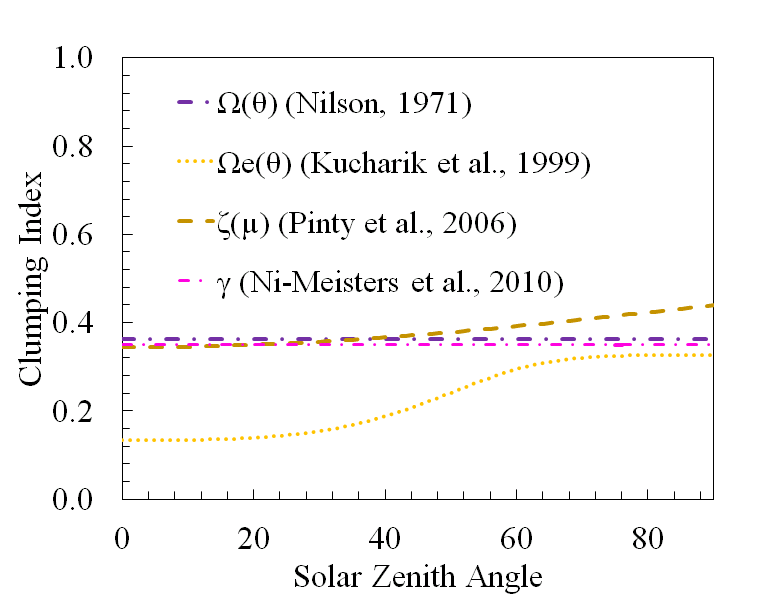
\includegraphics[width=0.5\textwidth]{/home/mn811042/Thesis/chapter4/figures/CI_comparison_050_v2.png}
                         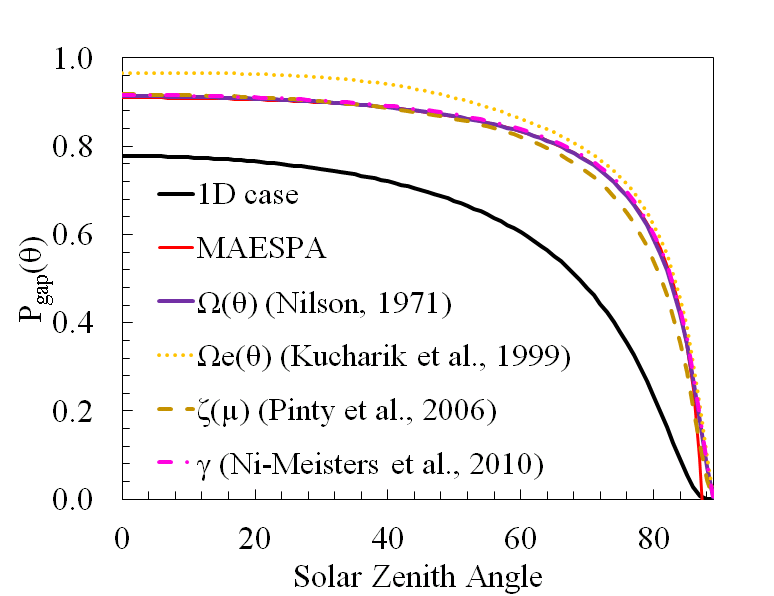
\includegraphics[width=0.5\textwidth]{/home/mn811042/Thesis/chapter4/figures/pgap_comparison_050.png}}
\end{tabular}

\begin{tabular}{ll}
\subfloat[Medium Canopy]{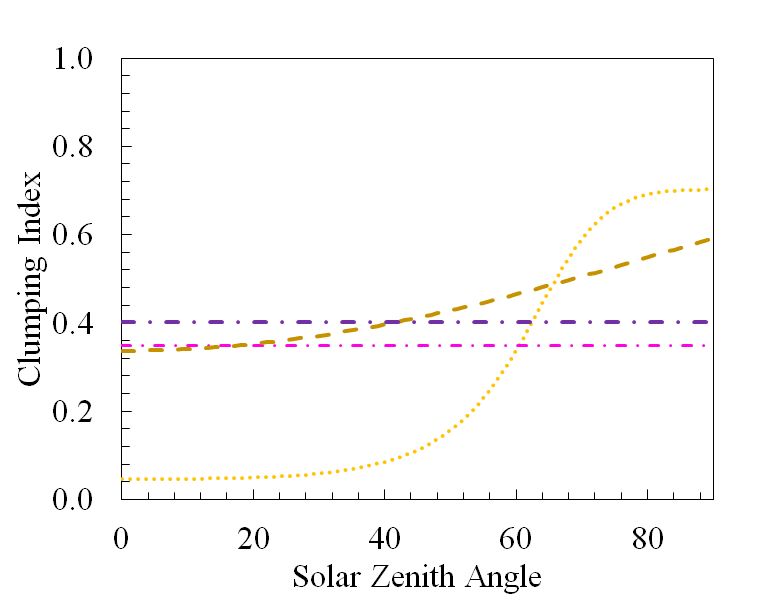
\includegraphics[width=0.5\textwidth]{/home/mn811042/Thesis/chapter4/figures/CI_comparison_150_v2.png}
                         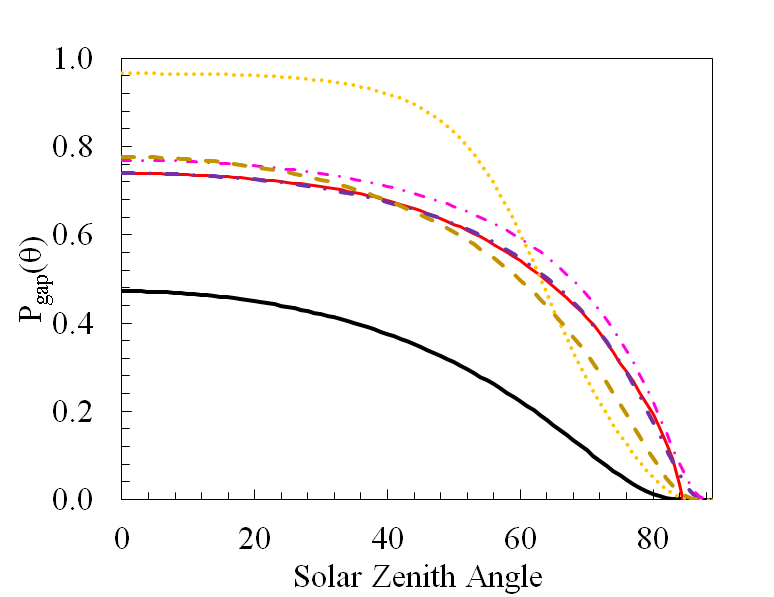
\includegraphics[width=0.5\textwidth]{/home/mn811042/Thesis/chapter4/figures/pgap_comparison_150.png}}
\end{tabular}

\begin{tabular}{ll}
\subfloat[Dense Canopy]{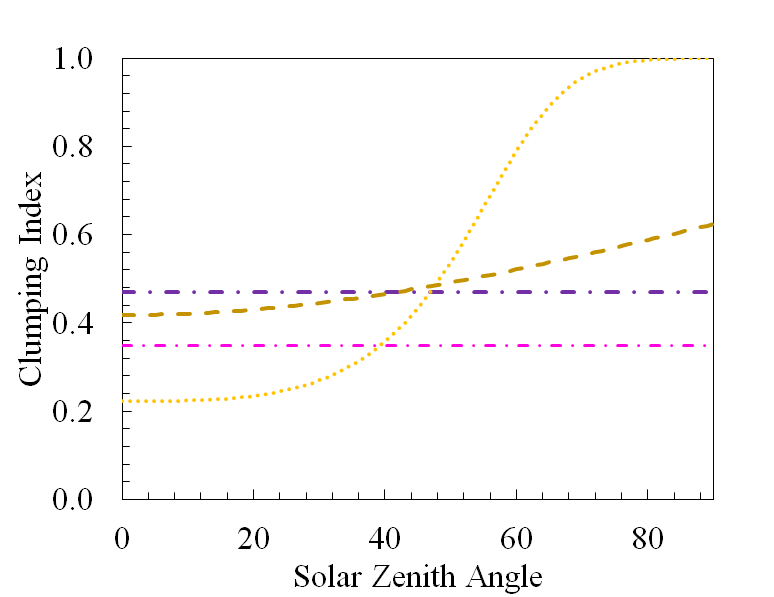
\includegraphics[width=0.5\textwidth]{/home/mn811042/Thesis/chapter4/figures/CI_comparison_250_v2.png}
                        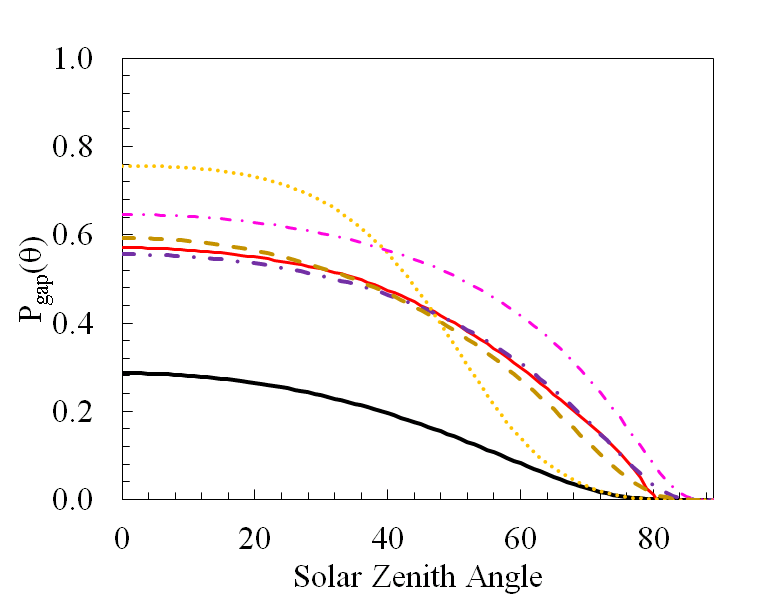
\includegraphics[width=0.5\textwidth]{/home/mn811042/Thesis/chapter4/figures/pgap_comparison_250.png}}
\end{tabular}

\caption{Comparison between different ways to calculate clumping index and its impact on gap fraction.}
\label{f:ci_comparisons}
\end{figure}

The clumping index of \citet{Nilson1971} was directly inverted from the P$_{gap}(\theta)$ curve as the angular coefficient of the linear adjust. This value is a single number, which does not vary with zenith angle, and it is represented as a straight parallel line with the x-axis in Figure~\ref{f:ci_comparisons}(left). As represented in Figure~\ref{f:ci_comparisons}(right), Nilson\textquotesingle s clumping index gives a very good agreement with the calculated P$_{gap}(\theta)$ from the 3D model, as it was fitted against the results. The total RMSE from this index is at the order of 0.15 for the sparse canopy, increasing with canopy density, until up to 0.27 for the dense case (Figure~\ref{fig:ci_rmse}).

To calculate the \citet{Kucharik1999} clumping index, it is necessary first to know the number of stems within a determined ground area; second, the crown diameter, and third, the ratio of crown depth to crown diameter. Besides that, this clumping index parameterisation scheme is a semi-empirical equation adjusted for a specific set of data collected in the Canadian boreal forests during the BOREAS experiment. Its applicability could not necessarily be extended to other plant functional types, especially because it takes into account the element clumping index related to shoots, exclusive to needle-leaf tree species.

For the sparse canopy, P$_{gap}(\theta)$ obtained with Kucharik\textquotesingle s method tend to overestimate the reference values by 10\% through the range of evaluated solar zenith angles until about 60$^{\circ}$. For higher solar zenith angles direct transmissivity calculated with this parameterisation agrees well with the reference values obtained with the 3D model.

The \citet{Kucharik1999} parameterisation presents a clumping index always smaller than the other two for the sparse canopy, showing a triple behaviour with a varying zenith angle. From 0$^{\circ}$ to 20$^{\circ}$ the clumping index is approximately constant and equals to 0.15, which indicates a large discrepancy between the 1D and the 3D cases. From 40$^{\circ}$ to 60$^{\circ}$, the clumping index increases following approximately a linear relationship with solar zenith angle. After 60$^{\circ}$, the clumping index reaches a second plateau in about 0.35.

For the sparse case, Figure~\ref{fig:ci_rmse} indicates that between the three evaluated parameterisation schemes, \citet{Kucharik1999} shows a slightly larger deviation from the 3D model reference values ($\approx$ 0.15), but still a smaller deviation than the 1D case, which supports the fact that applying the clumping index correction improves the direct transmissivity calculations.

For the medium canopy, the clumping index also presents the same triple behaviour (i.e., plateau - linear relationship - plateau), but for this case, with a very distinct behaviour than the other two evaluated parameterisations schemes.

From 0$^{\circ}$ to about 40$^{\circ}$, the clumping index is very small ($\approx$ 0.0), which results in a direct transmissivity of approximately 1.0, or 25\% higher than the 3D reference model. From 40$^{\circ}$ to 70$^{\circ}$, the clumping index presents a rapid increase reaching the second plateau in about P$_{gap}(\theta)$ = 0.7, and it underestimates the 3D reference model at the end of the solar zenith angle range.

For the same medium scenario, this parameterisation scheme showed a performance not as accurate as the other two, when compared with the 3D reference model, but still better than the 1D case in average.

In the dense canopy (LAI = 2.5 m$^2$.m$^{-2}$), the Kucharik\textquotesingle s parameterisation scheme behaves only slightly more deviant than the other two in the average by evaluating the RMSE obtained with the 3D model reference values. The behaviour of the clumping index curve with solar zenith angle is about the same than in the other two canopy densities, but with $\Omega(\theta) = 1.0$ at the end of the solar zenith angle range (from 70$^{\circ}$ to 85$^{\circ}$). From this analysis, it is possible to say, for this part of the solar zenith range, that this parameterisation scheme gives similar results than the 1D case. Between all three canopy densities, however, the use of Kucharik\textquotesingle s parameterisation scheme results in a smaller error, when compared to the 3D reference model in comparison to the 1D case. The relationship for the clumping index of \citet{Ni-Meister2010} is based on an analytical expression, which can also only be determined with previous knowledge about stem density, crown radius, and scene LAI. Besides that, the generalised equation for spheres does not depend on Sun zenith angle, and was constant for the evaluated scenarios ($\gamma \approx 0.35$).

The variable that determines the clumping index from \citet{Ni-Meister2010} is $\tau_0r$, which is proportional to LAI and $\lambda$ (Eq.~\ref{equation:clumpNi}). For the RAMI4PILPS scenarios, LAI and $\lambda$ increase at the same proportion, and as a result, the clumping index for all three scenes was kept constant, but without greatly compromising the final direct transmissivity. In the average, Ni-Meister\textsinglequote s clumping index fairly agreed with the reference model for all three canopy densities. Over all evaluated cases, Ni-Meister\textquotesingle s parameterisation showed a better agreement with the reference model than the 1D case, specifically for the medium case. For the dense case, Ni-Meister\textquotesingle s parameterisation scheme overestimates the reference P$_{gap}(\theta)$ along all solar zenith angles in about 10\%. Overall, this parameterisation scheme seemed to give similar results to the 3D model reference values. By using the structure factor parameterisation \citep{pinty2006}, there is no need to have previous knowledge about canopy structure; the parameters are minimised against terms of the radiation partitioning (absorbance, reflectance and/or transmittance), either measured, or calculated by detailed radiative transfer schemes (Section~\ref{section:pintyscheme}). Overall, the structure factor presented the best agreement with the 3D model reference values of P$_{gap}(\theta)$, together with the other minimised clumping index of Nilson.

For the sparse and medium cases, the structure factor presents close values to the clumping index of \citet{Nilson1971} and \citet{Ni-Meister2010} for small solar zenith angles, i.e., smaller than 40$^{\circ}$ for the sparse case, and smaller than 20$^{\circ}$ for the medium case. However, the difference is in the fact that the structure factor increases with solar zenith angle, which can be interpreted as the radiation path length gets longer with a lower Sun in the sky.

By comparing the gap probability generated with four different clumping indices with the one generated by the MAESPA model, the ones that were minimised against the original 3D modelled data presented the lowest averaged RMSE (Figure~\ref{fig:ci_rmse}), i.e., the clumping index of \citet{Nilson1971}, and the structure factor of \citet{pinty2006}. 

These two indices are empirical, and they could be applied to any type of vegetation canopy without previous knowledge about structure, once they were minimised against the modelled data. In the case of \citet{Nilson1971}, the clumping index was minimised against direct transmissivity only; and in the case of \citet{pinty2006}, the structure factor was minimised against the reference values of fAPAR and albedo PAR together for each canopy density separately. The RMSE results are summarised in Figure~\ref{f:ci_comparisons}(left).

%In the following sections, the clumping indices are used in further evaluations of the radiation partitioning within the two-stream approximation. First, using the modified two-stream scheme, 4 different clumping indices are compared against the RAMI4PILPS reference values, and against other 3D models, for absorption and reflectance in two distinct narrow spectral bands, PAR (400 - 700 nm) and NIR (700 - 3000 nm).

\begin{figure}
\centering
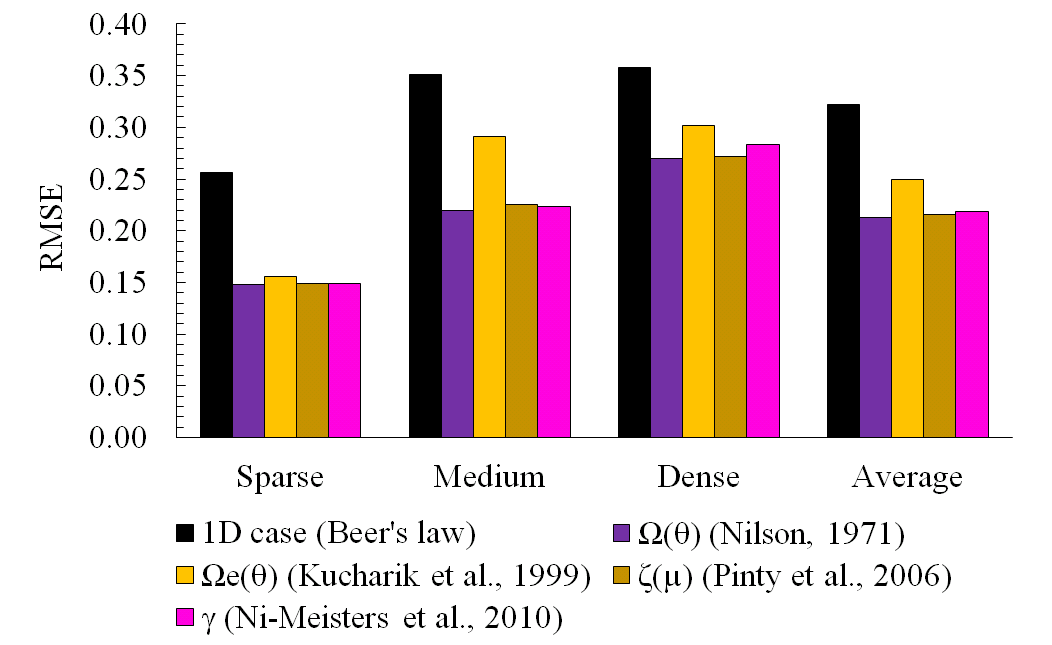
\includegraphics[width=1.0\textwidth]{/home/mn811042/Thesis/chapter4/figures/CI_rmse_v2.png}
\caption{Root-Mean-Squared-Error of gap probability generated with three structural parameterisations and MAESPA for three different canopies densities (sparse, medium and dense) and the average.} 
\label{fig:ci_rmse}
\end{figure}

\section{Evaluating vegetation structural effects in the two-stream scheme: zenith profile}

This section uses four radiative transfer models, the modified version of the two-stream scheme with four different clumping indices, and a parameterisation scheme of the two-stream scheme commonly used in LSMs to obtain the zenith profile of shortwave radiation partitioning in two distinct wavebands, PAR and NIR, for vegetation canopy scenes described in the RAMI4PILPS experiment.

The RAMI4PILPS reference values of absorption and reflectance were calculated through a 3D radiative transfer model based on a Monte Carlo ray-tracing approach, raytran \citep{Govaerts1995}. Two other radiative transfer models, MAESPA \citep{Wang1990,Medlyn2004,Medlyn2007}, and GORT \citep{Li1995,Ni1997}, both 3D radiative transfer models, were also used in this exercise in order to compare different radiative transfer methodologies to describe heterogeneous vegetation canopies.

The performance of the 1D radiative transfer scheme, two-stream approximation \citep{Sellers1985}, is tested in this exercise. Also, in order to evaluate an approach often implemented in GCMs to account for sparse vegetation canopies, a commonly used parameterisation based on the amount of vegetation fraction cover on a model grid cell is also applied, referred as Veg$_{frac}$.

Finally, four different clumping indices were implemented in the modified version of the two-stream scheme, and their ability to calculate shortwave radiation partitioning are compared, as well. These are the clumping indices schemes developed by: 1) \citet{Nilson1971}; 2) \citet{Kucharik1999}; 3) the `structure factor' parameterisation scheme of \citet{pinty2006}, and; 4) the clumping index of \citet{Ni-Meister2010}, developed from the GORT model.

The following subsections present the results for absorption and reflectance separately, over PAR and NIR spectral regions in Figures~\ref{f:szacomparisonfPAR}, \ref{f:szacomparisonfNIR}, \ref{f:szacomparisonalbPAR}, and \ref{f:szacomparisonalbNIR}.

\subsection{Absorption}

The two-stream scheme overestimates the reference values for PAR absorption over all evaluated canopy densities, under both illumination conditions, i.e., direct and diffuse. This behaviour indicates that this scheme is more optically opaque for PAR radiation than the 3D Monte Carlo ray-tracing reference model, particularly due to canopy architectural impacts on radiation propagation. This result is in agreement with the evaluation performed in Section~\ref{section:lai}, where the two-stream scheme overestimates absorption for all different canopy structures generated by the MAESPA model with same total scene LAI. 

In the NIR spectrum, the two-stream scheme presents a relative good agreement with the reference values for absorption, especially for solar zenith angles equal to 60$^{\circ}$, and under a diffuse illumination condition. For other cases, the two-stream scheme overestimates the reference values for smaller solar zenith angles (until $\approx$ 27.5$^{\circ}$), and the opposite, i.e., underestimates it for higher solar zenith angles ($\approx$ 83.5$^{\circ}$).

MAESPA shows good results in calculating PAR absorption for different vegetation canopy densities. It strongly agreed with the RAMI4PILPS reference values for PAR absorption, but only over non-bright surfaces. This particular result indicates that MAESPA as a trustworthy tool, that could be used in future experiments related to PAR absorption. In the snow case (SNW), however, MAESPA underestimates PAR absorption in up to 30\% over the dense canopy, which demonstrates the limitations of this model in dealing with background reflectance. Overall, the MAESPA model can be used in future intercomparison exercises related to PAR absorption, but its results should be carefully evaluated over highly reflective surfaces. In the NIR spectrum, MAESPA was able to reproduce the shape of the curve associated with absorption, but underestimated the reference values by up to 10\% in a dense canopy over snow.

Also evaluated in this study, the GORT model presented good agreement with the RAMI4PILPS reference values for the sparse case scenario over all soil reflectances, for direct illumination. The best fit agreement with the reference values are found in the solar zenith angle range going from 0$^{\circ}$ to 60$^{\circ}$, in the PAR spectral region. For higher solar zenith angles, GORT underestimates PAR absorption by up to 20\% over a black soil background. For diffuse illumination, the GORT model agrees with the reference values. As canopy density increases, PAR absorption generated by the GORT model starts to be underestimated, especially over snow ($\alpha_{soil}$ = 0.96), for direct and diffuse illumination conditions. In the NIR spectrum, GORT presented a persistent overestimation in absorption for both illumination conditions.

The commonly used parameterisation based on fraction of vegetation cover, or Veg$_{frac}$ correction is not able to reproduce the PAR, or NIR absorption. It underestimates the total PAR absorption over all evaluated cases. This result is particularly important, because it shows the limited ability of LSMs in correctly estimate PAR absorption used for photosynthesis calculations. Greater discrepancies are associated with higher Sun zenith angles ($>$ 30$^{\circ}$).

With regards to the parameterisation schemes, Figure~\ref{f:szacomparisonfPAR} indicates that overall the structure factor parameterisation scheme \citep{pinty2006} consistently showed a better agreement to the RAMI4PILPS reference values than any other approach under direct (Solar Zenith Angles from 0 to 90$^{\circ}$), and diffuse illumination conditions. It seemed to be an accurate tool to derive PAR absorption for all evaluated scenarios, with especial attention to its performance over a brighter background (SNW case). The very good agreement with the reference values over snow can be explained for the fact that the minimisation process has been done over all soil brightness together, and the different highly scattering behaviour of PAR over snow worked as an `attractor' for the structure factor parameters.

In the PAR region, the clumping index of \citet{Nilson1971} shows a good agreement with the structure factor over the sparse case scenario, and for small Sun zenith angles ($<$ 30$^{\circ}$), but as canopy density increases, and for higher Sun zenith angles ($>$ 30$^{\circ}$), the clumping index of \citet{Nilson1971} is not able to reproduce the complete behaviour of more complex models for absorption, which indicates that by considering a variant clumping index with Sun zenith angle as in \citet{pinty2006}, the modified two-stream scheme can match the results of 3D models more accurately. 

Following this explanatory analysis between the total difference in radiation partitioning with regards of having or not a zenith dependent clumping index, the main difference between the clumping indices of \citet{pinty2006} and \citet{Ni-Meister2010} is also related to the presence of clumping index angular variability. Figure~\ref{f:ci_comparisons} shows that for the sparse and medium cases, both clumping indices are basically the same until approximately a solar zenith angle of 25$^{\circ}$; after that value, the structure factor based on \citet{pinty2006} increases with Sun zenith angle. For the dense case, the structure factor is about 5\% lager than the clumping index of \citet{Ni-Meister2010} at the begging of the zenith angular range. The intercomparison between these two clumping indices, and their effects on shortwave radiation partitioning when applied to the two-stream approach reinforces the evaluation of wether or not considering an angular variant clumping index is important. 

For the sparse case, the differences between Pinty and Ni-Meister\textquotesingle s schemes are roughly limited to a small curvature between 60$^{\circ}$ and 80$^{\circ}$. As it can be seen in Figure~\ref{f:ci_comparisons}, the P$_{gap}$ calculated through both methods agreed quite well for most zenith angles, and present a RMSE = 0.15. So, for the sparse case, the consideration of a variant clumping index is not crucial to determine absolute values, or the curvature shape of PAR absorption with Sun zenith angle. The remaining parameterisation scheme of \citet{Kucharik1999} underestimates the values of PAR, and NIR absorption, while it overestimates the direct transmittance (Figure~\ref{f:ci_comparisons}).

The larger discrepancies between the three parameterisation schemes, however, appears when evaluating the medium and dense scenarios. While Ni-Meister\textquotesingle s scheme underestimates the reference values for all evaluated scenes, the most prominent differences are related to higher Sun zenith angles. Nevertheless, these differences are not observed when evaluating Pinty\textquotesingle s scheme, because the structure factor varies with Sun zenith angle.

Pinty\textquotesingle s parameterisation scheme is an efficient, and accurate tool to derive PAR absorption over all evaluated scenarios, with especial attention to its performance over a brighter background (snow), and over high zenith angles. Nilson\textquotesingle s parameterisation scheme has also been proved to be a robust tool to consider vegetation heterogeneity into a 1D radiative transfer model, with a not as good agreement over high Sun zenith angles. Followed by Ni-Meister\textquotesingle s parameterisation scheme that adds a lot of information into the two-stream scheme, by considering vegetation structural heterogeneity's; and even though the performance of the second is not as accurate as the first, it is better to add a clumping index into the two-stream approximation in order to consider structural variability, than do not add a clumping index. 

Kucharik\textquotesingle s parameterisation scheme has a different behaviour if compared with the other two, and presents a particular good agreement with the reference values for intermediate zenith angles, around 60$^{\circ}$. It is important to highlight that this specific parameterisation scheme was derived from observed data from boreal forests, which usually have non-spherical crowns, unlike the RAMI4PILPS canopies; and often presents needle-to-shoot clumping as well, which is not present in this exercise at all. 

\begin{figure}
\centering
\begin{tabular}{lll}
\subfloat[Sparse]{%\includegraphics[width=0.33\textwidth]{/home/mn811042/src/julesRT_struct_2/julesRT_struct/JULES_STRUCT_FACTOR/fabs_PAR_050_BLK_STRUC.png}
                  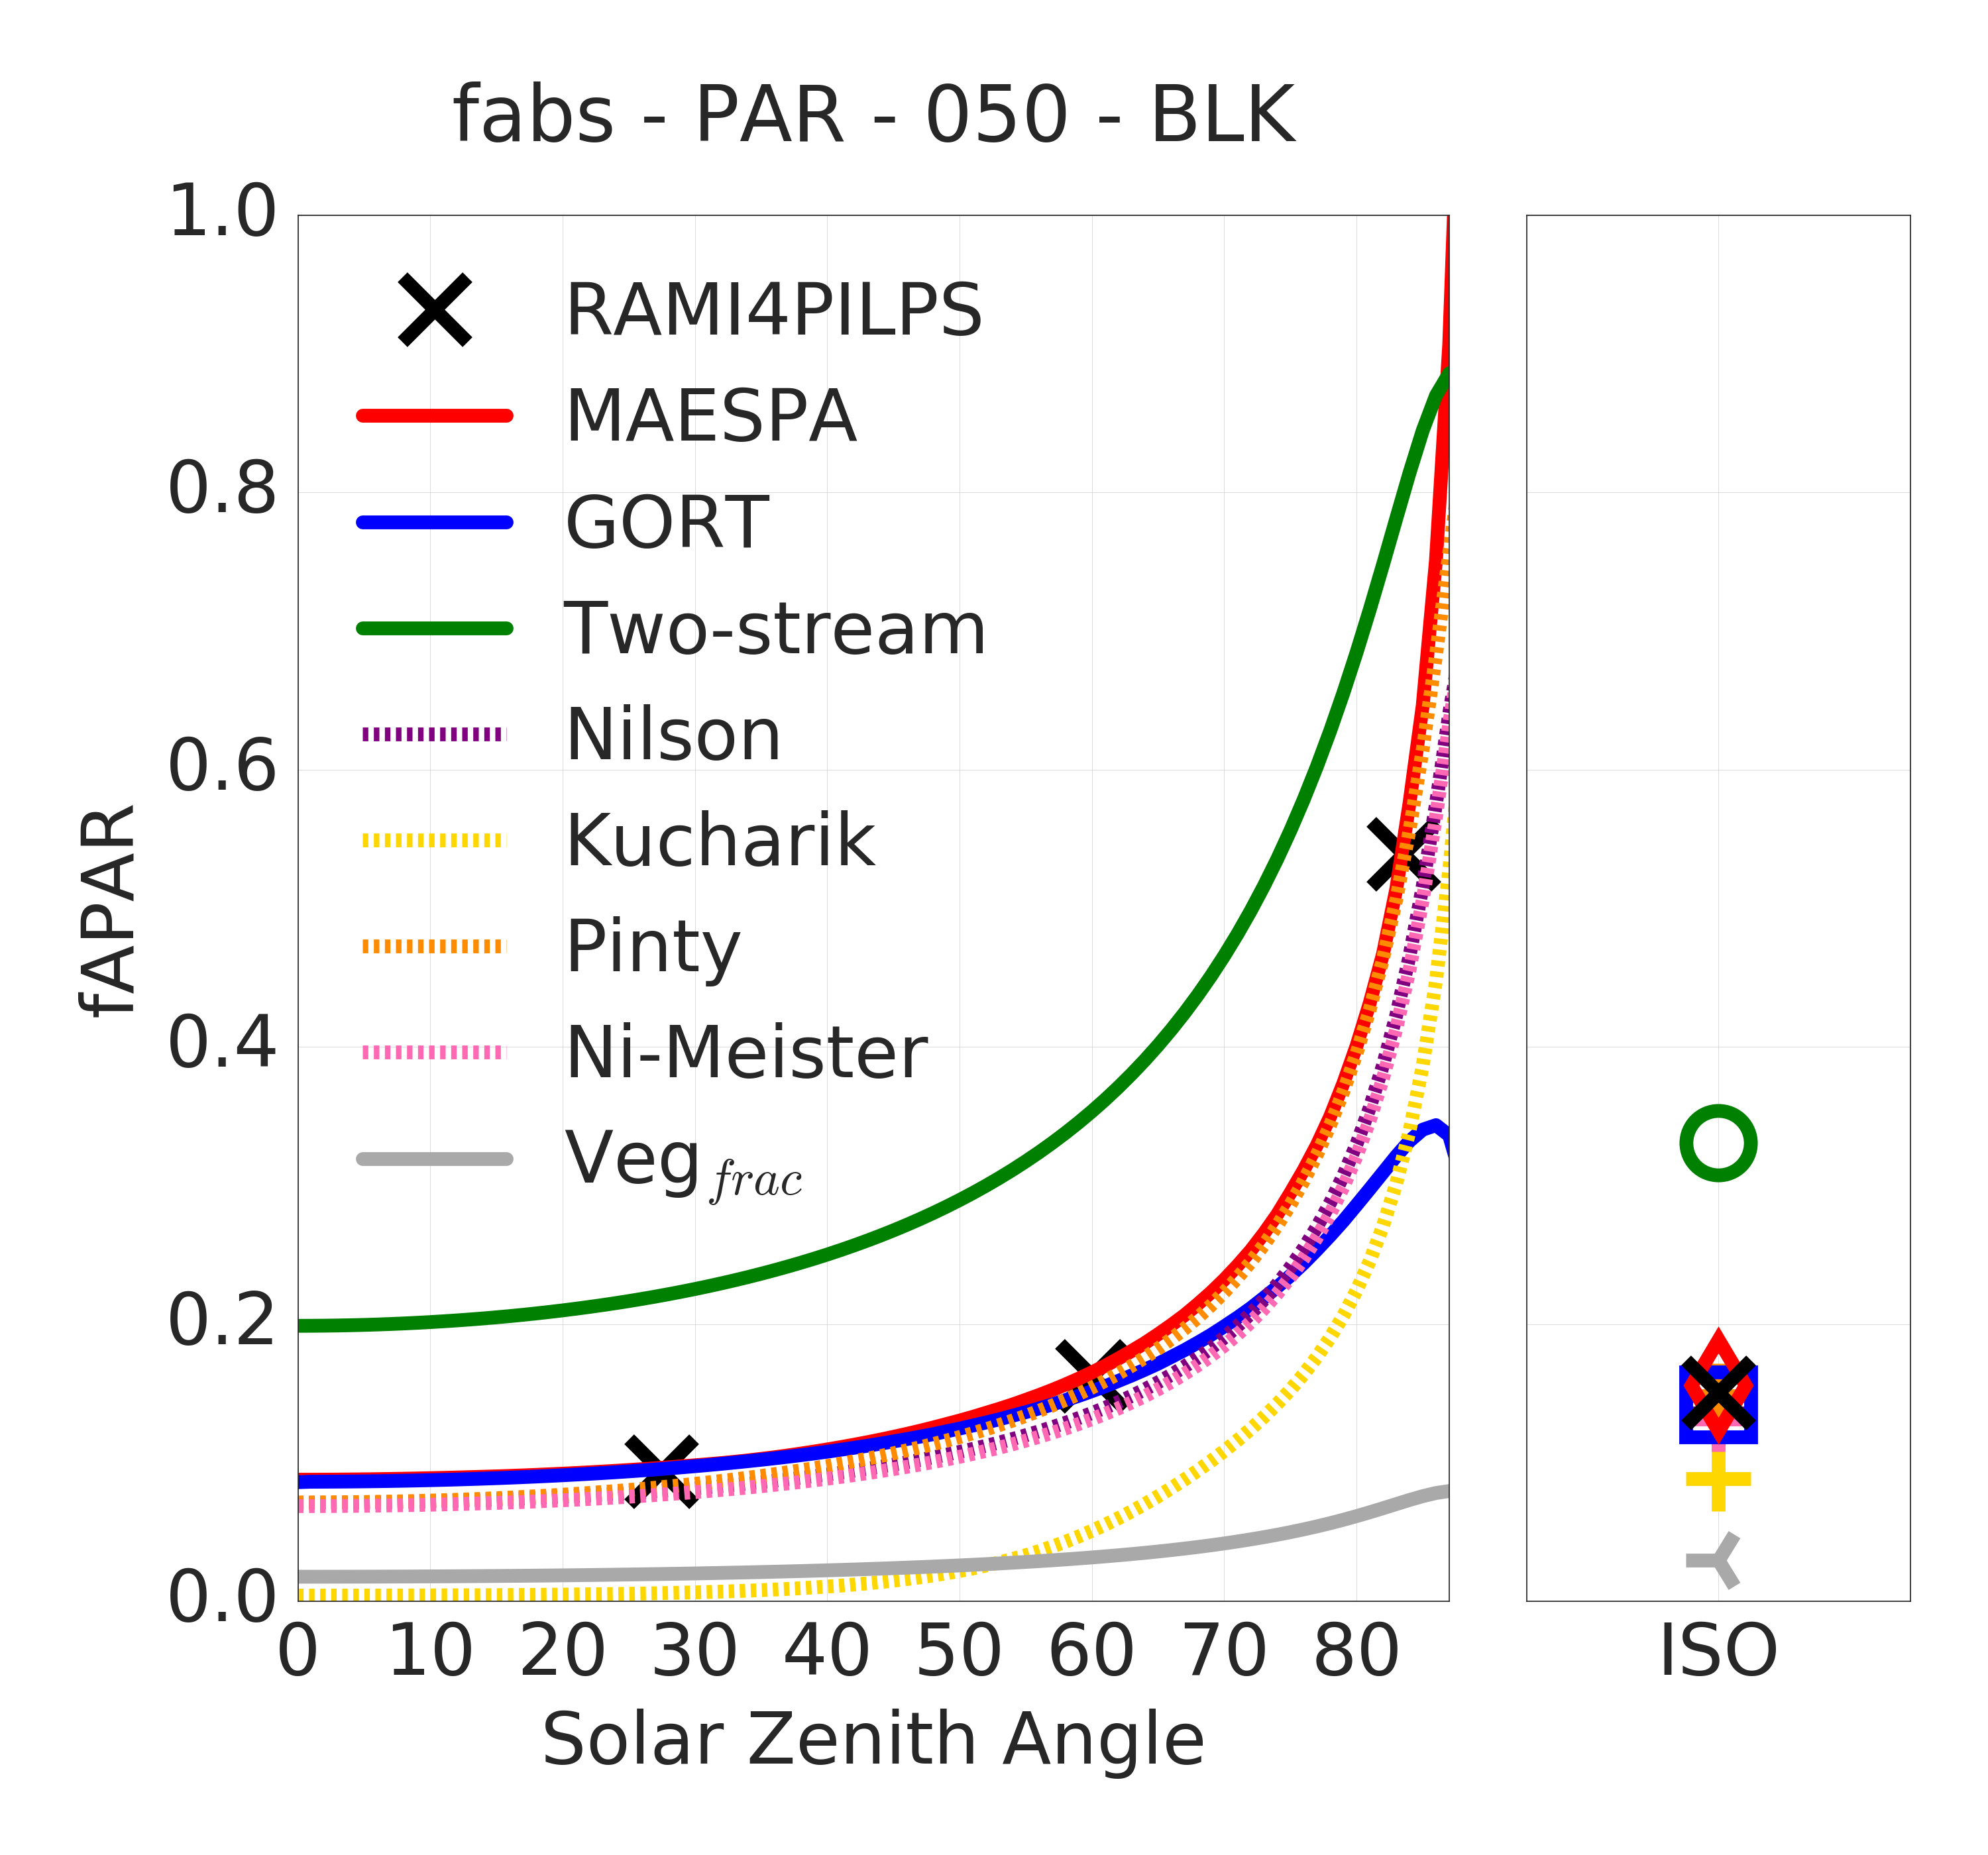
\includegraphics[width=0.33\textwidth]{/home/mn811042/src/julesRT_struct_2/julesRT_struct/data_comparison/figures/fapar_050_BLK.png}
                  %\includegraphics[width=0.33\textwidth]{/home/mn811042/src/julesRT_struct_2/julesRT_struct/JULES_STRUCT_FACTOR/fabs_PAR_050_MED_STRUC.png}
                  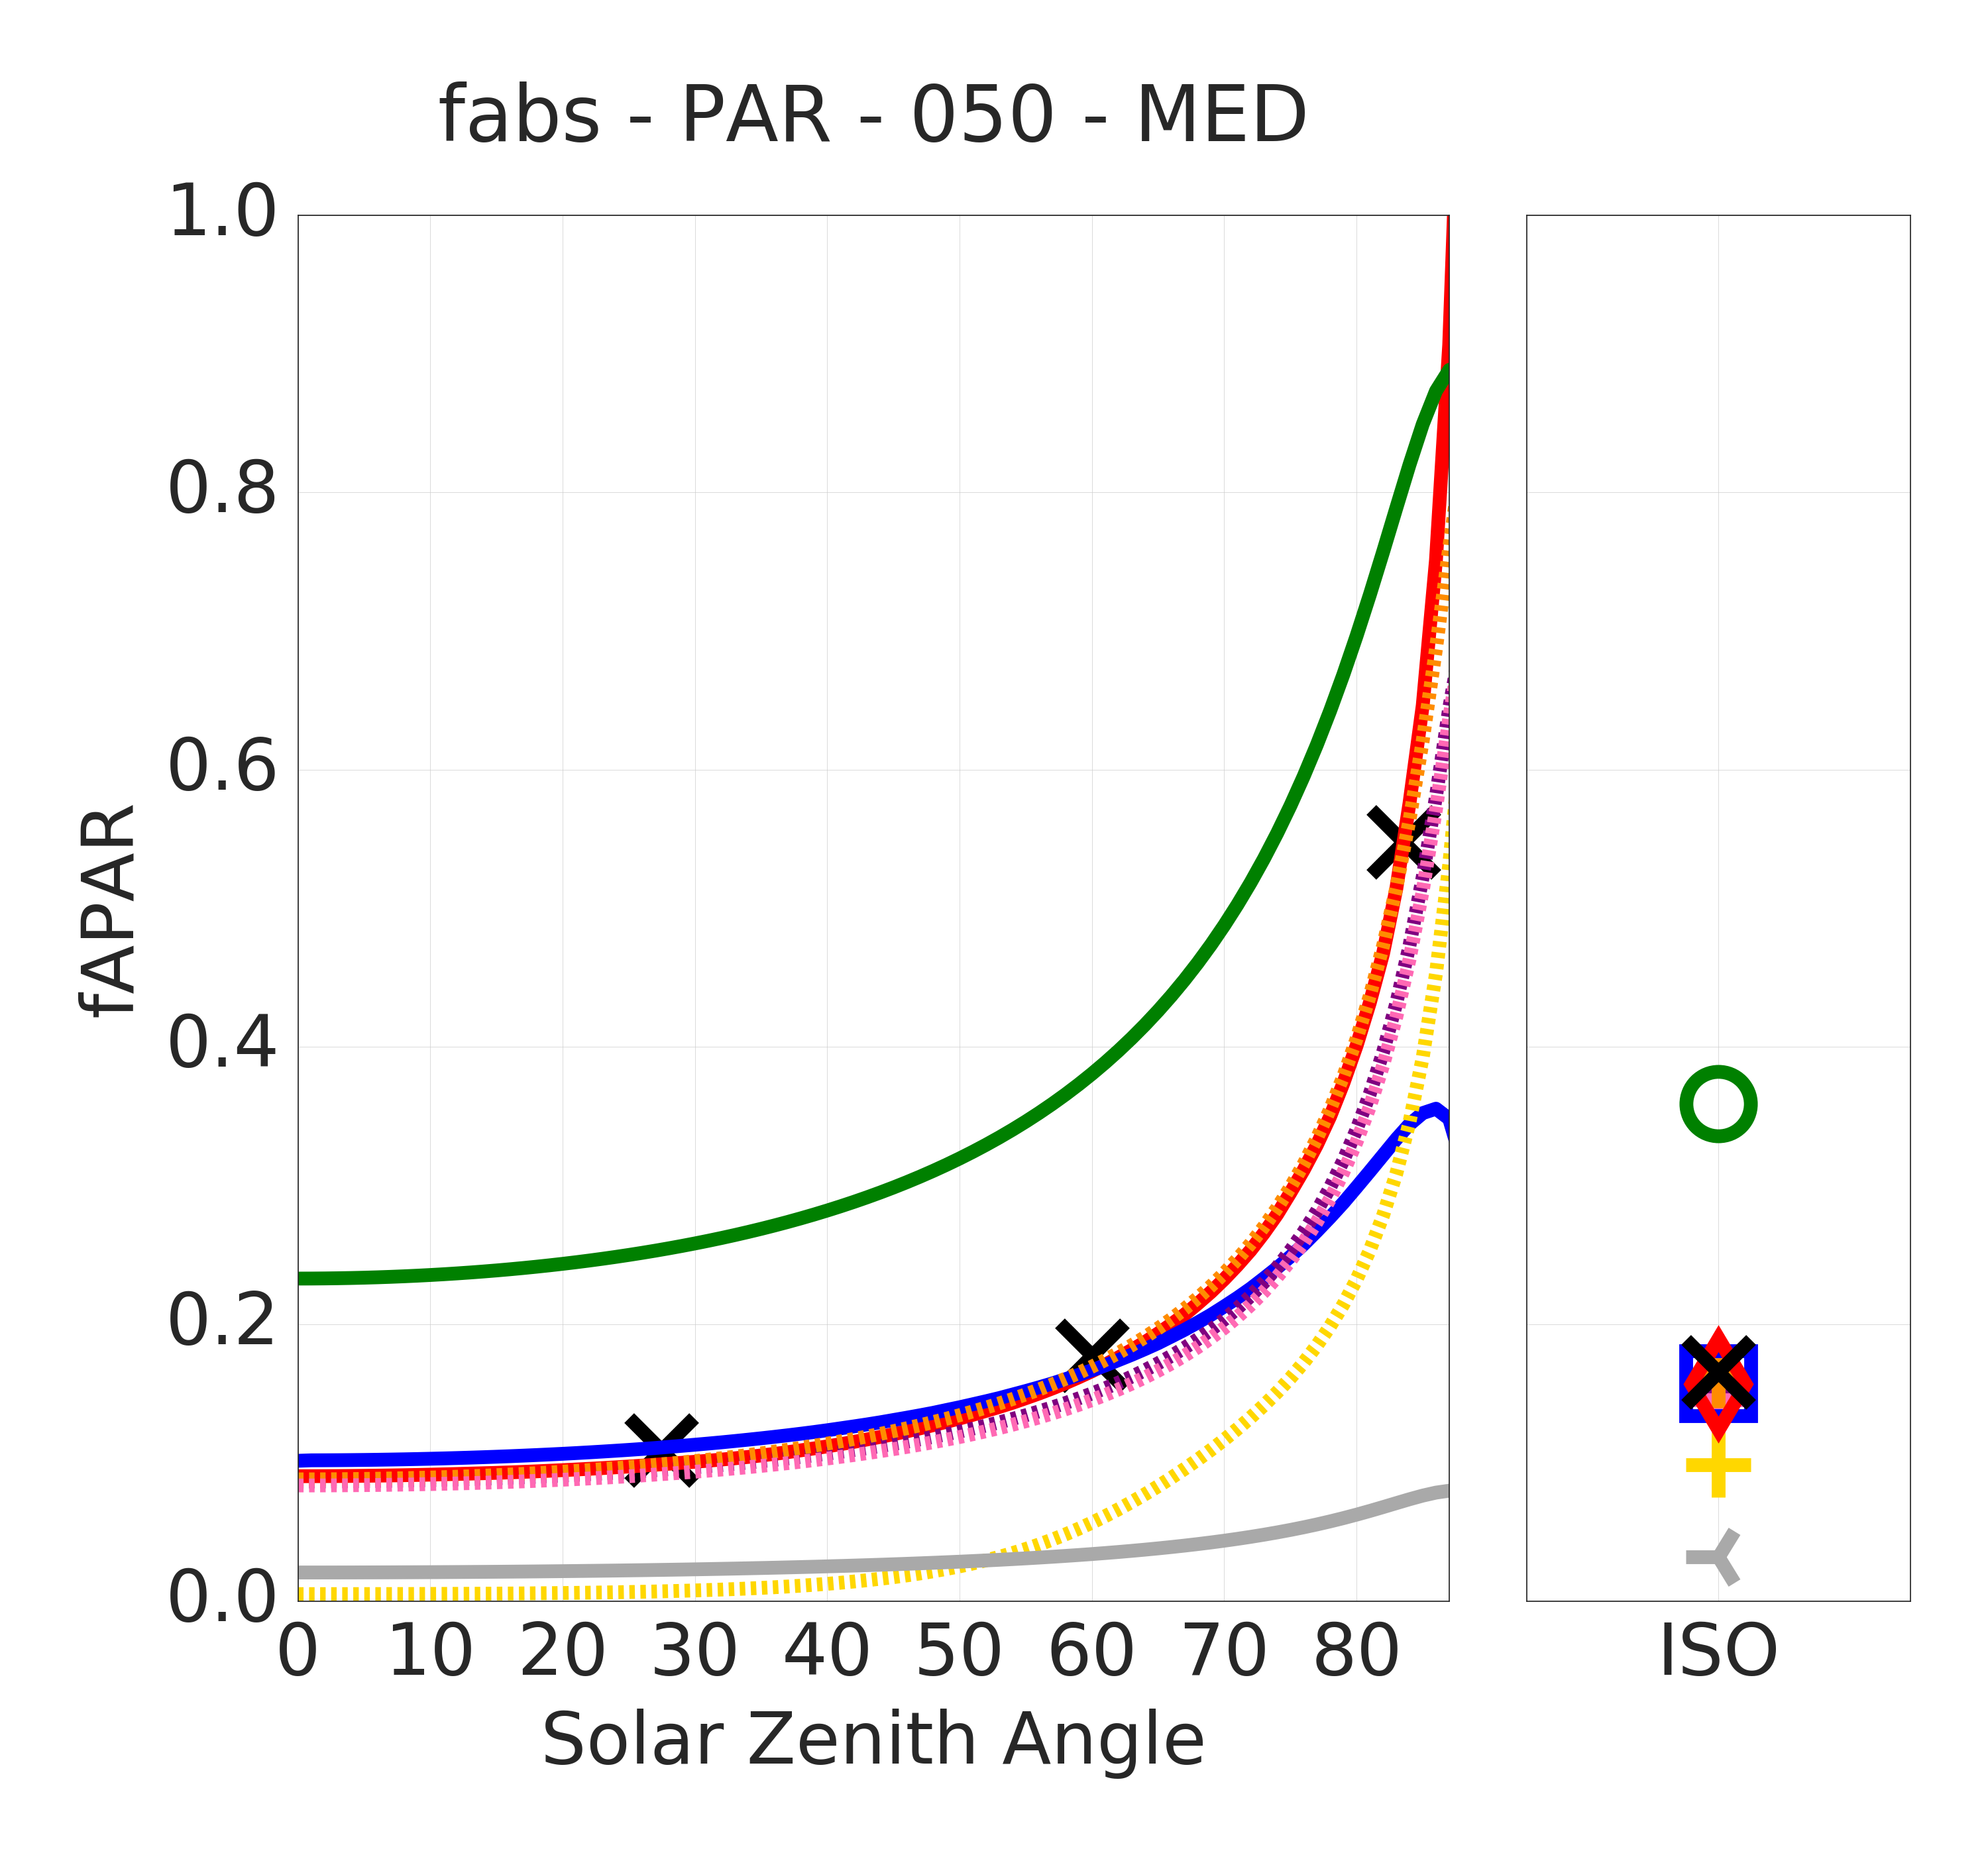
\includegraphics[width=0.33\textwidth]{/home/mn811042/src/julesRT_struct_2/julesRT_struct/data_comparison/figures/fapar_050_MED.png}
                  %\includegraphics[width=0.33\textwidth]{/home/mn811042/src/julesRT_struct_2/julesRT_struct/JULES_STRUCT_FACTOR/fabs_PAR_050_SNW_STRUC.png}}
                  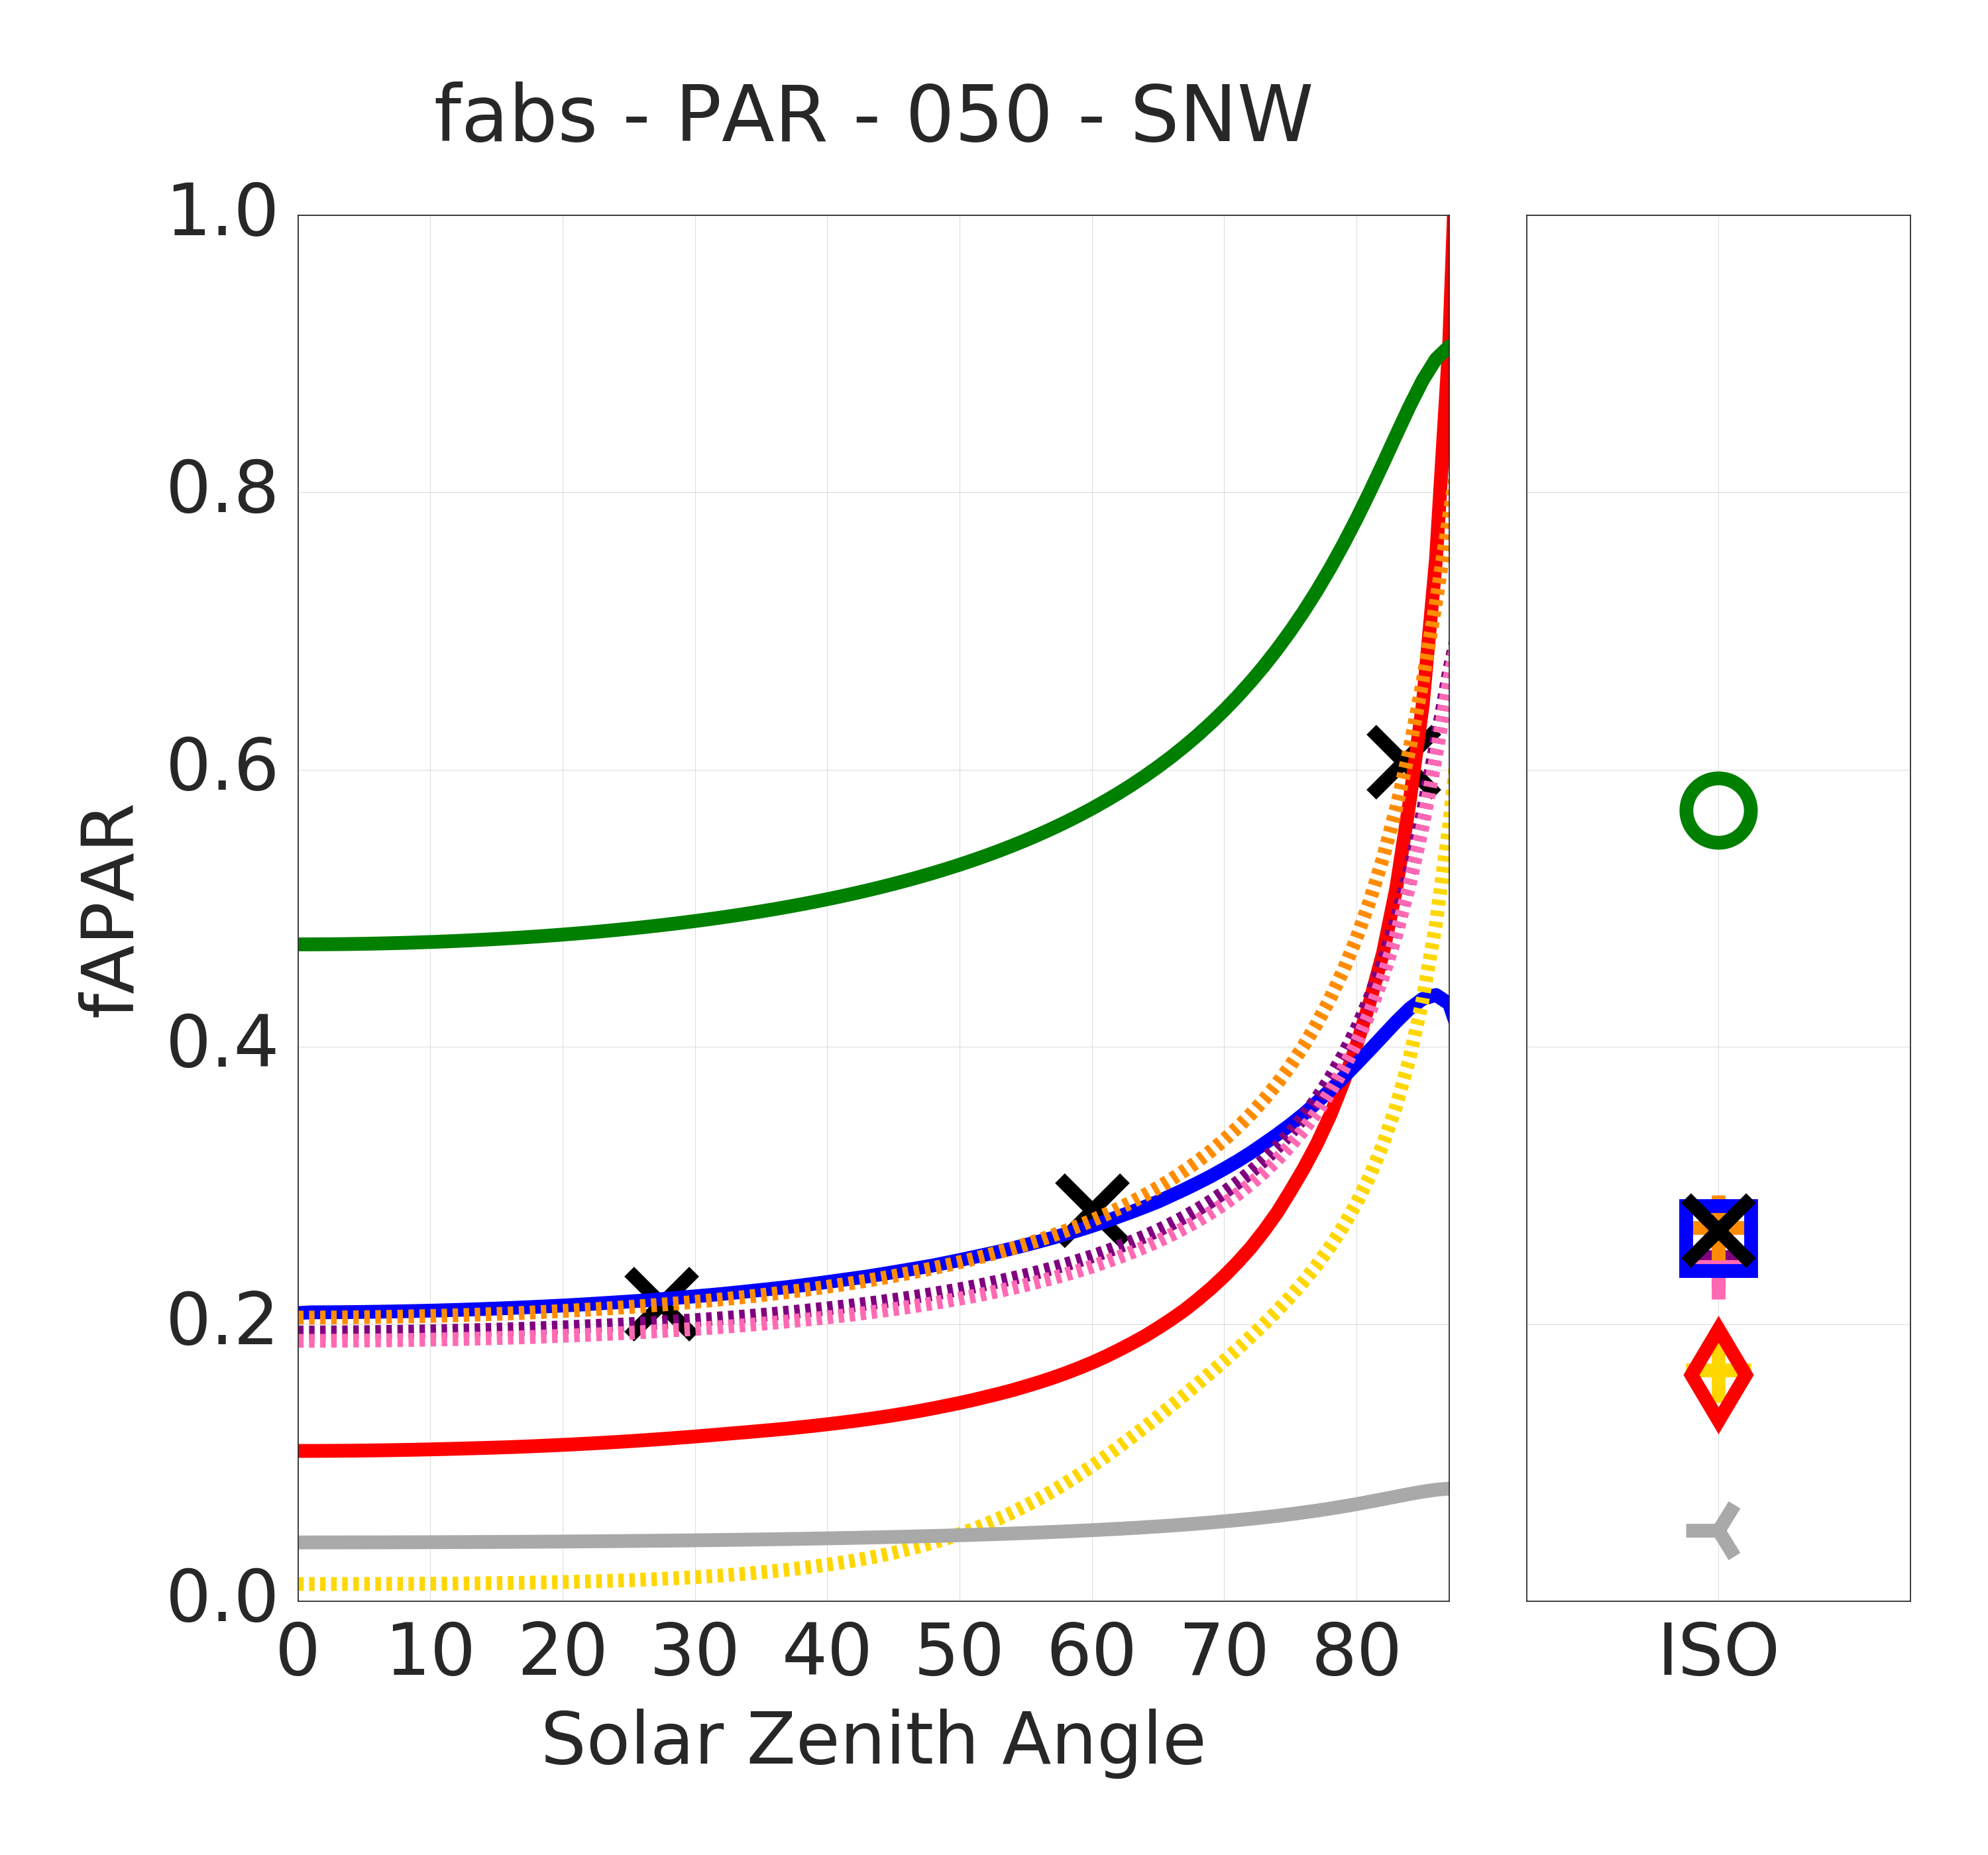
\includegraphics[width=0.33\textwidth]{/home/mn811042/src/julesRT_struct_2/julesRT_struct/data_comparison/figures/fapar_050_SNW.png}}
\end{tabular}
\begin{tabular}{lll}
\subfloat[Medium]{%\includegraphics[width=0.33\textwidth]{/home/mn811042/src/julesRT_struct_2/julesRT_struct/JULES_STRUCT_FACTOR/fabs_PAR_150_BLK_STRUC.png}
                  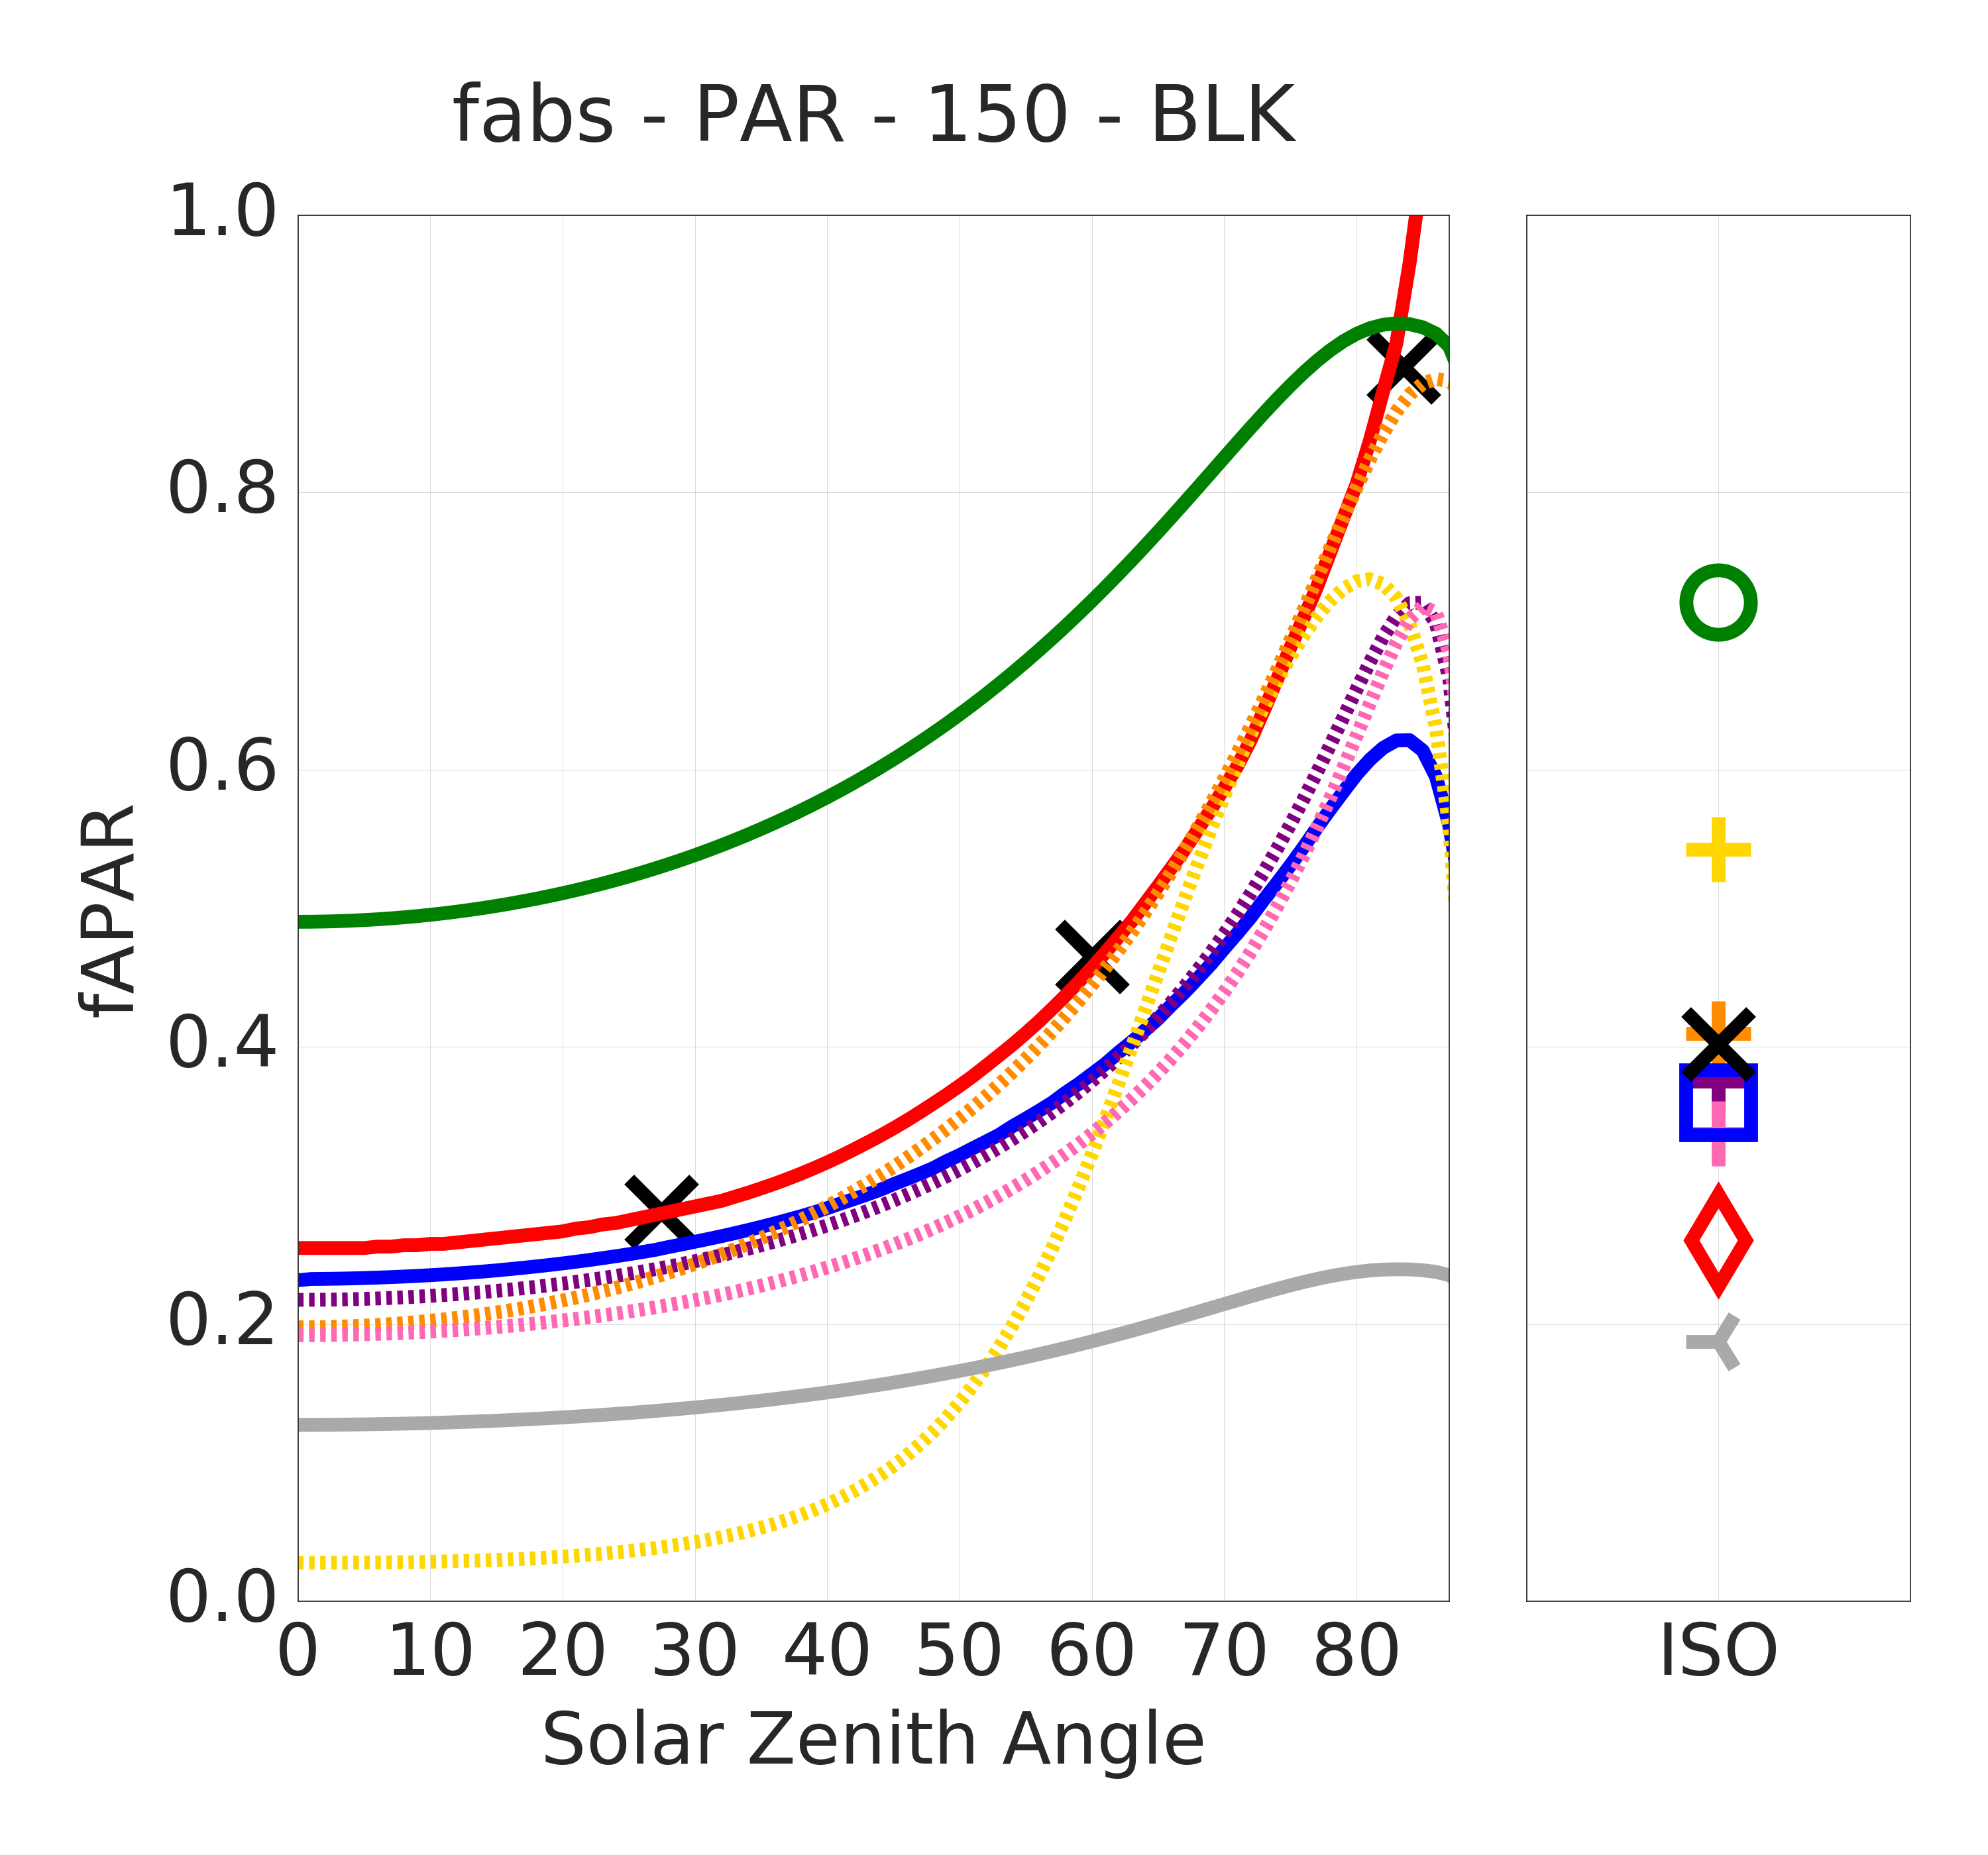
\includegraphics[width=0.33\textwidth]{/home/mn811042/src/julesRT_struct_2/julesRT_struct/data_comparison/figures/fapar_150_BLK.png}
                  %\includegraphics[width=0.33\textwidth]{/home/mn811042/src/julesRT_struct_2/julesRT_struct/JULES_STRUCT_FACTOR/fabs_PAR_150_MED_STRUC.png}
                  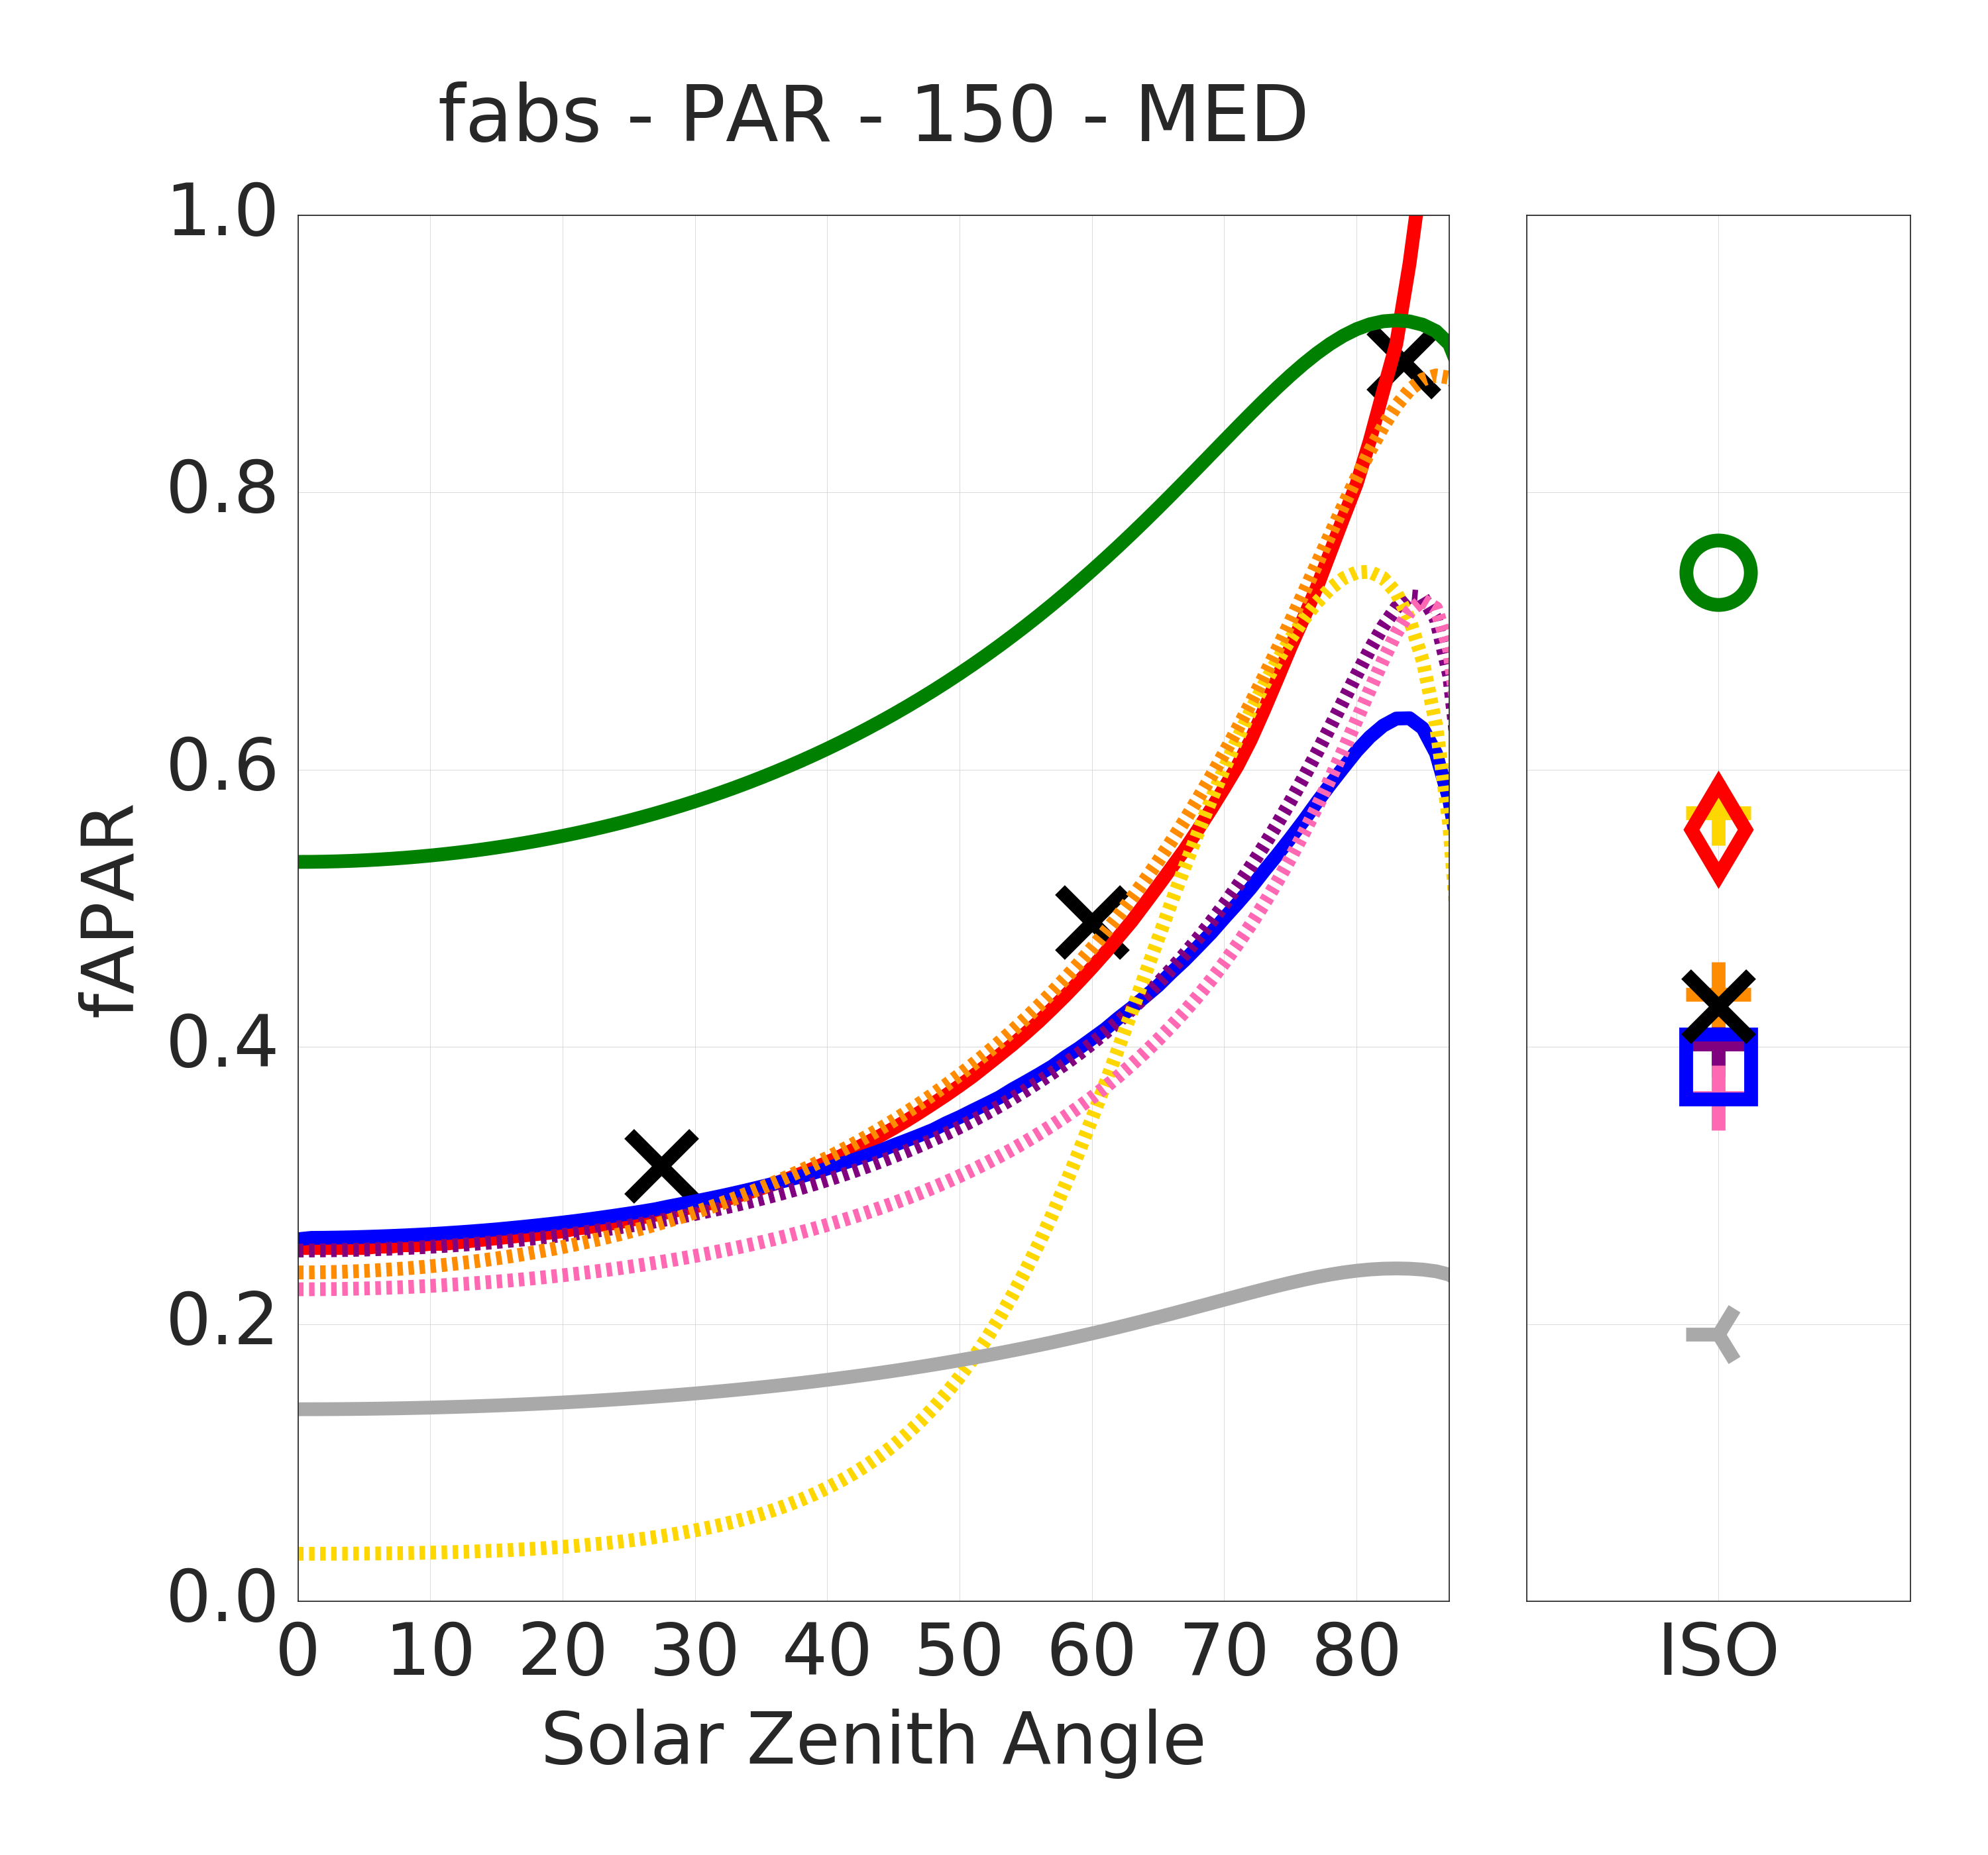
\includegraphics[width=0.33\textwidth]{/home/mn811042/src/julesRT_struct_2/julesRT_struct/data_comparison/figures/fapar_150_MED.png}
                  %\includegraphics[width=0.33\textwidth]{/home/mn811042/src/julesRT_struct_2/julesRT_struct/JULES_STRUCT_FACTOR/fabs_PAR_150_SNW_STRUC.png}} 
                  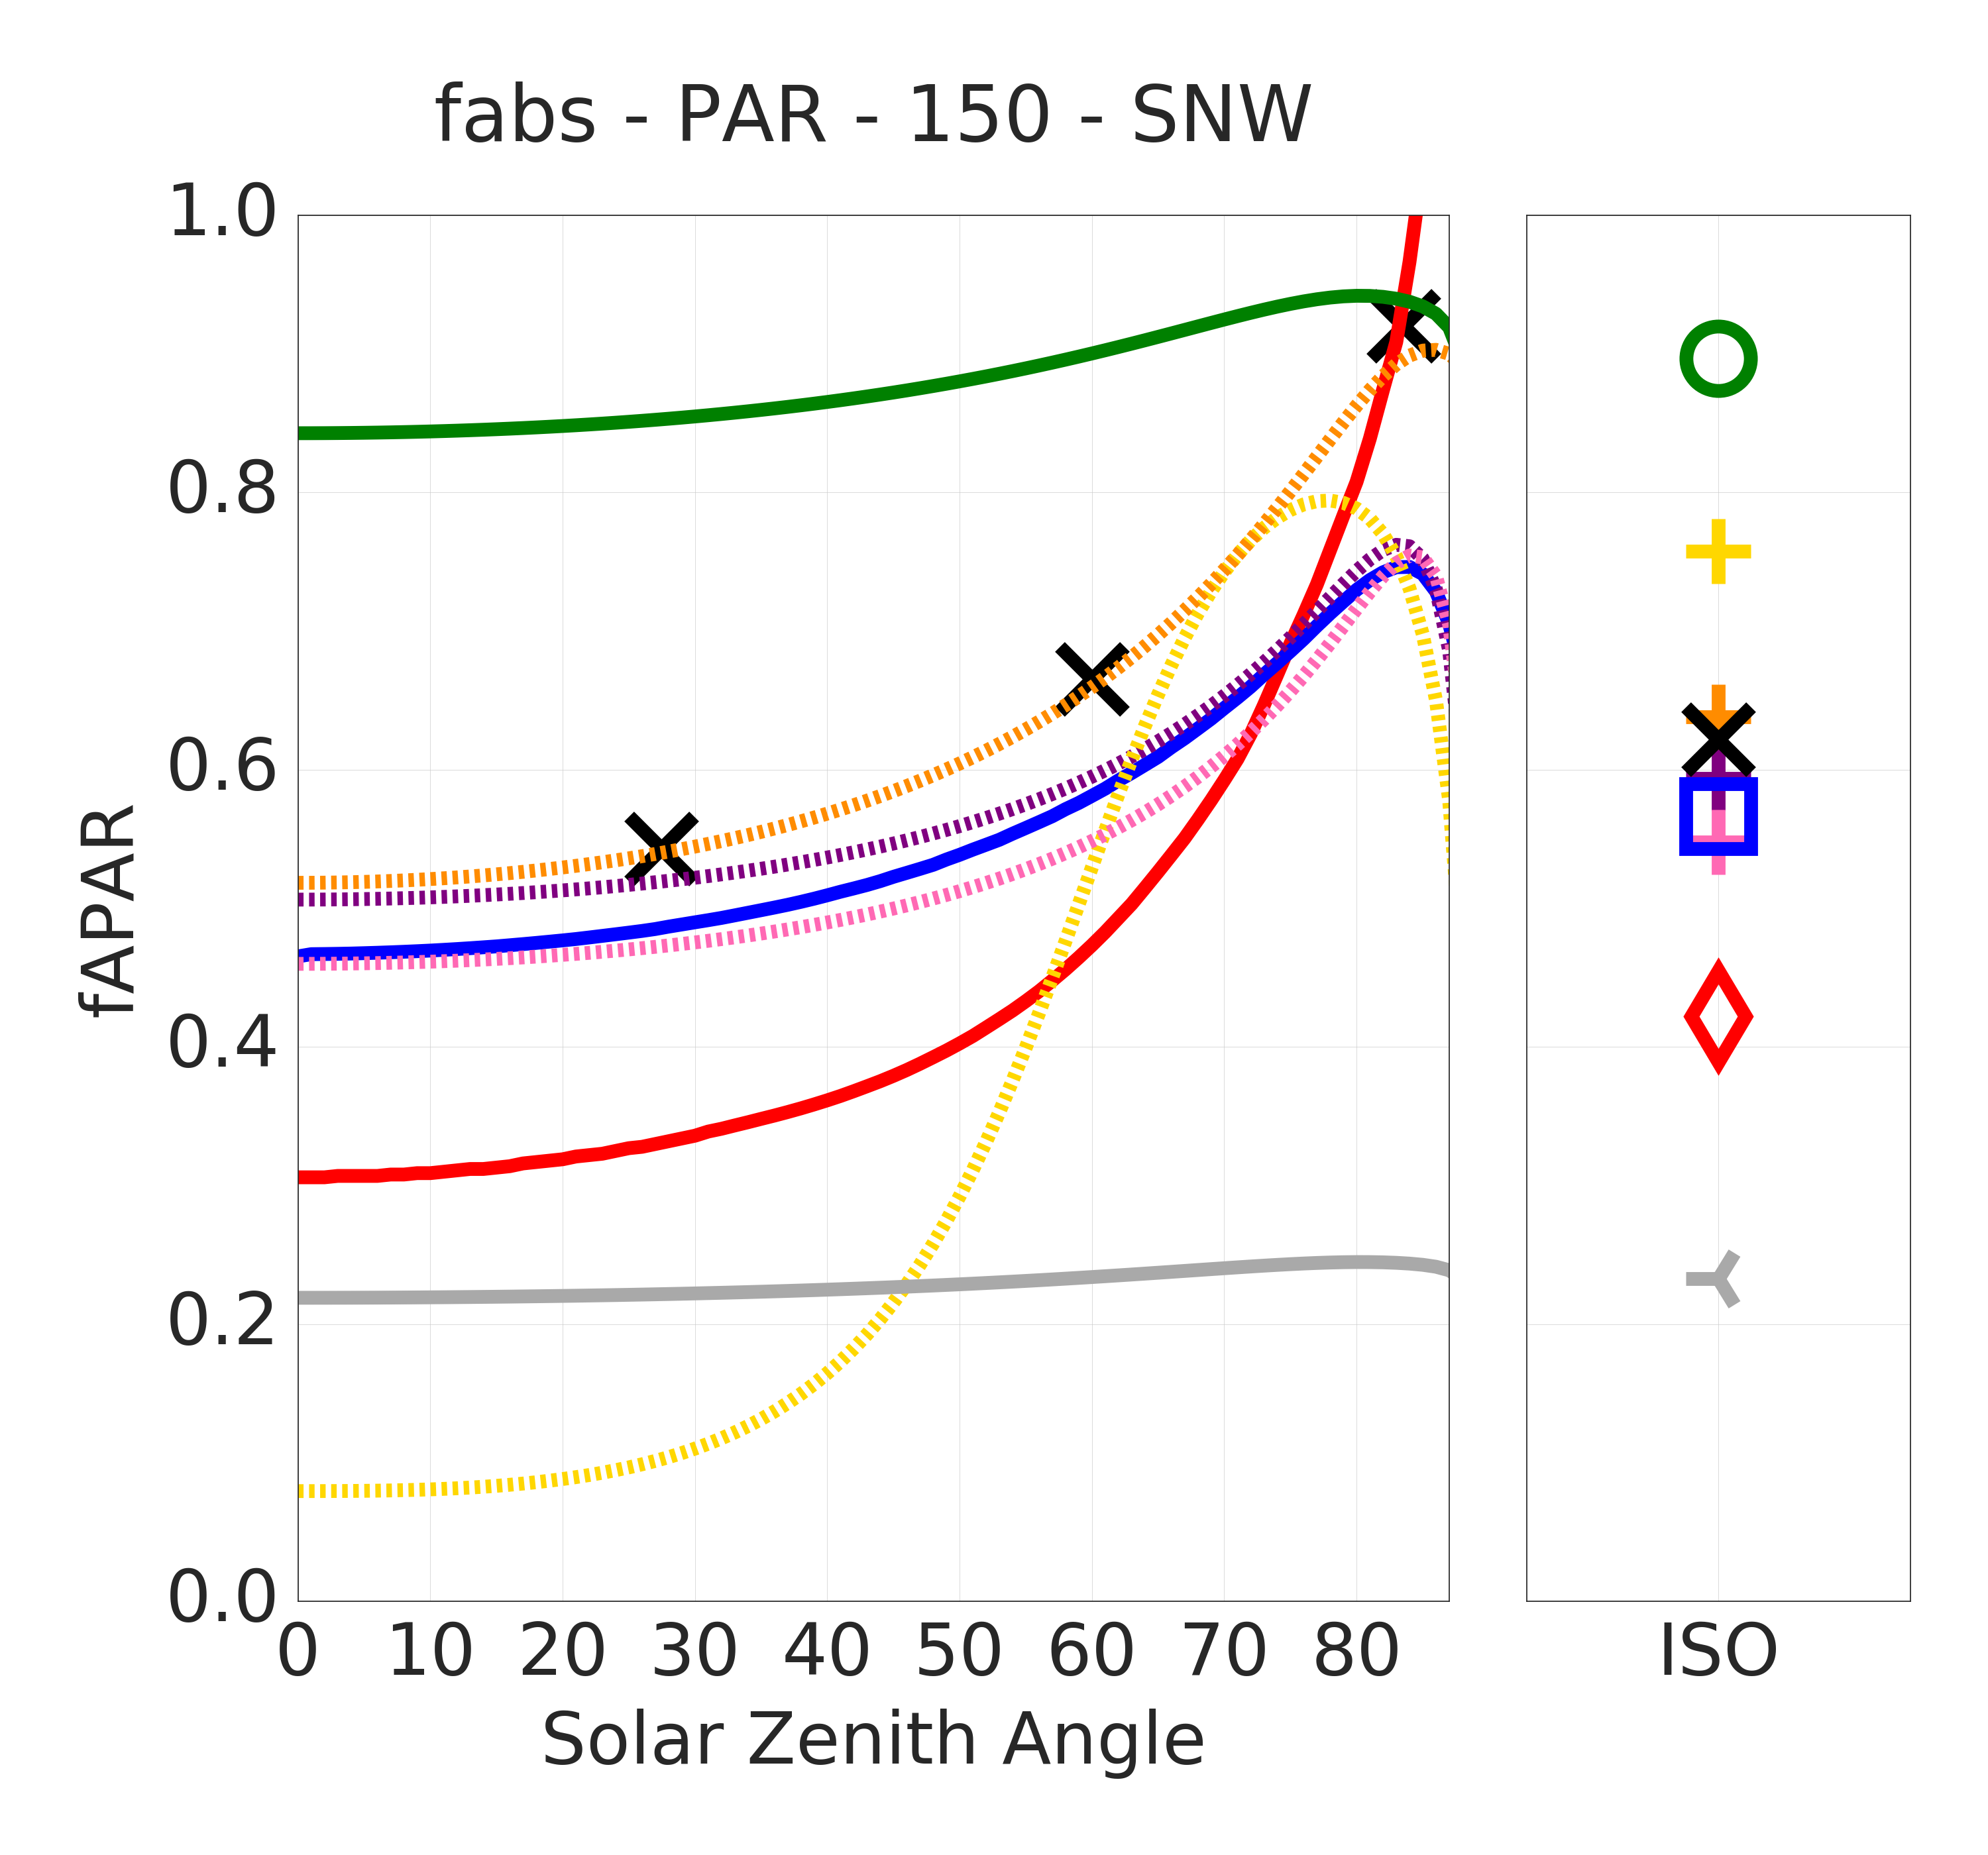
\includegraphics[width=0.33\textwidth]{/home/mn811042/src/julesRT_struct_2/julesRT_struct/data_comparison/figures/fapar_150_SNW.png}}
\end{tabular}
\begin{tabular}{lll}
\subfloat[Dense]{%\includegraphics[width=0.33\textwidth]{/home/mn811042/src/julesRT_struct_2/julesRT_struct/JULES_STRUCT_FACTOR/fabs_PAR_250_BLK_STRUC.png}
                 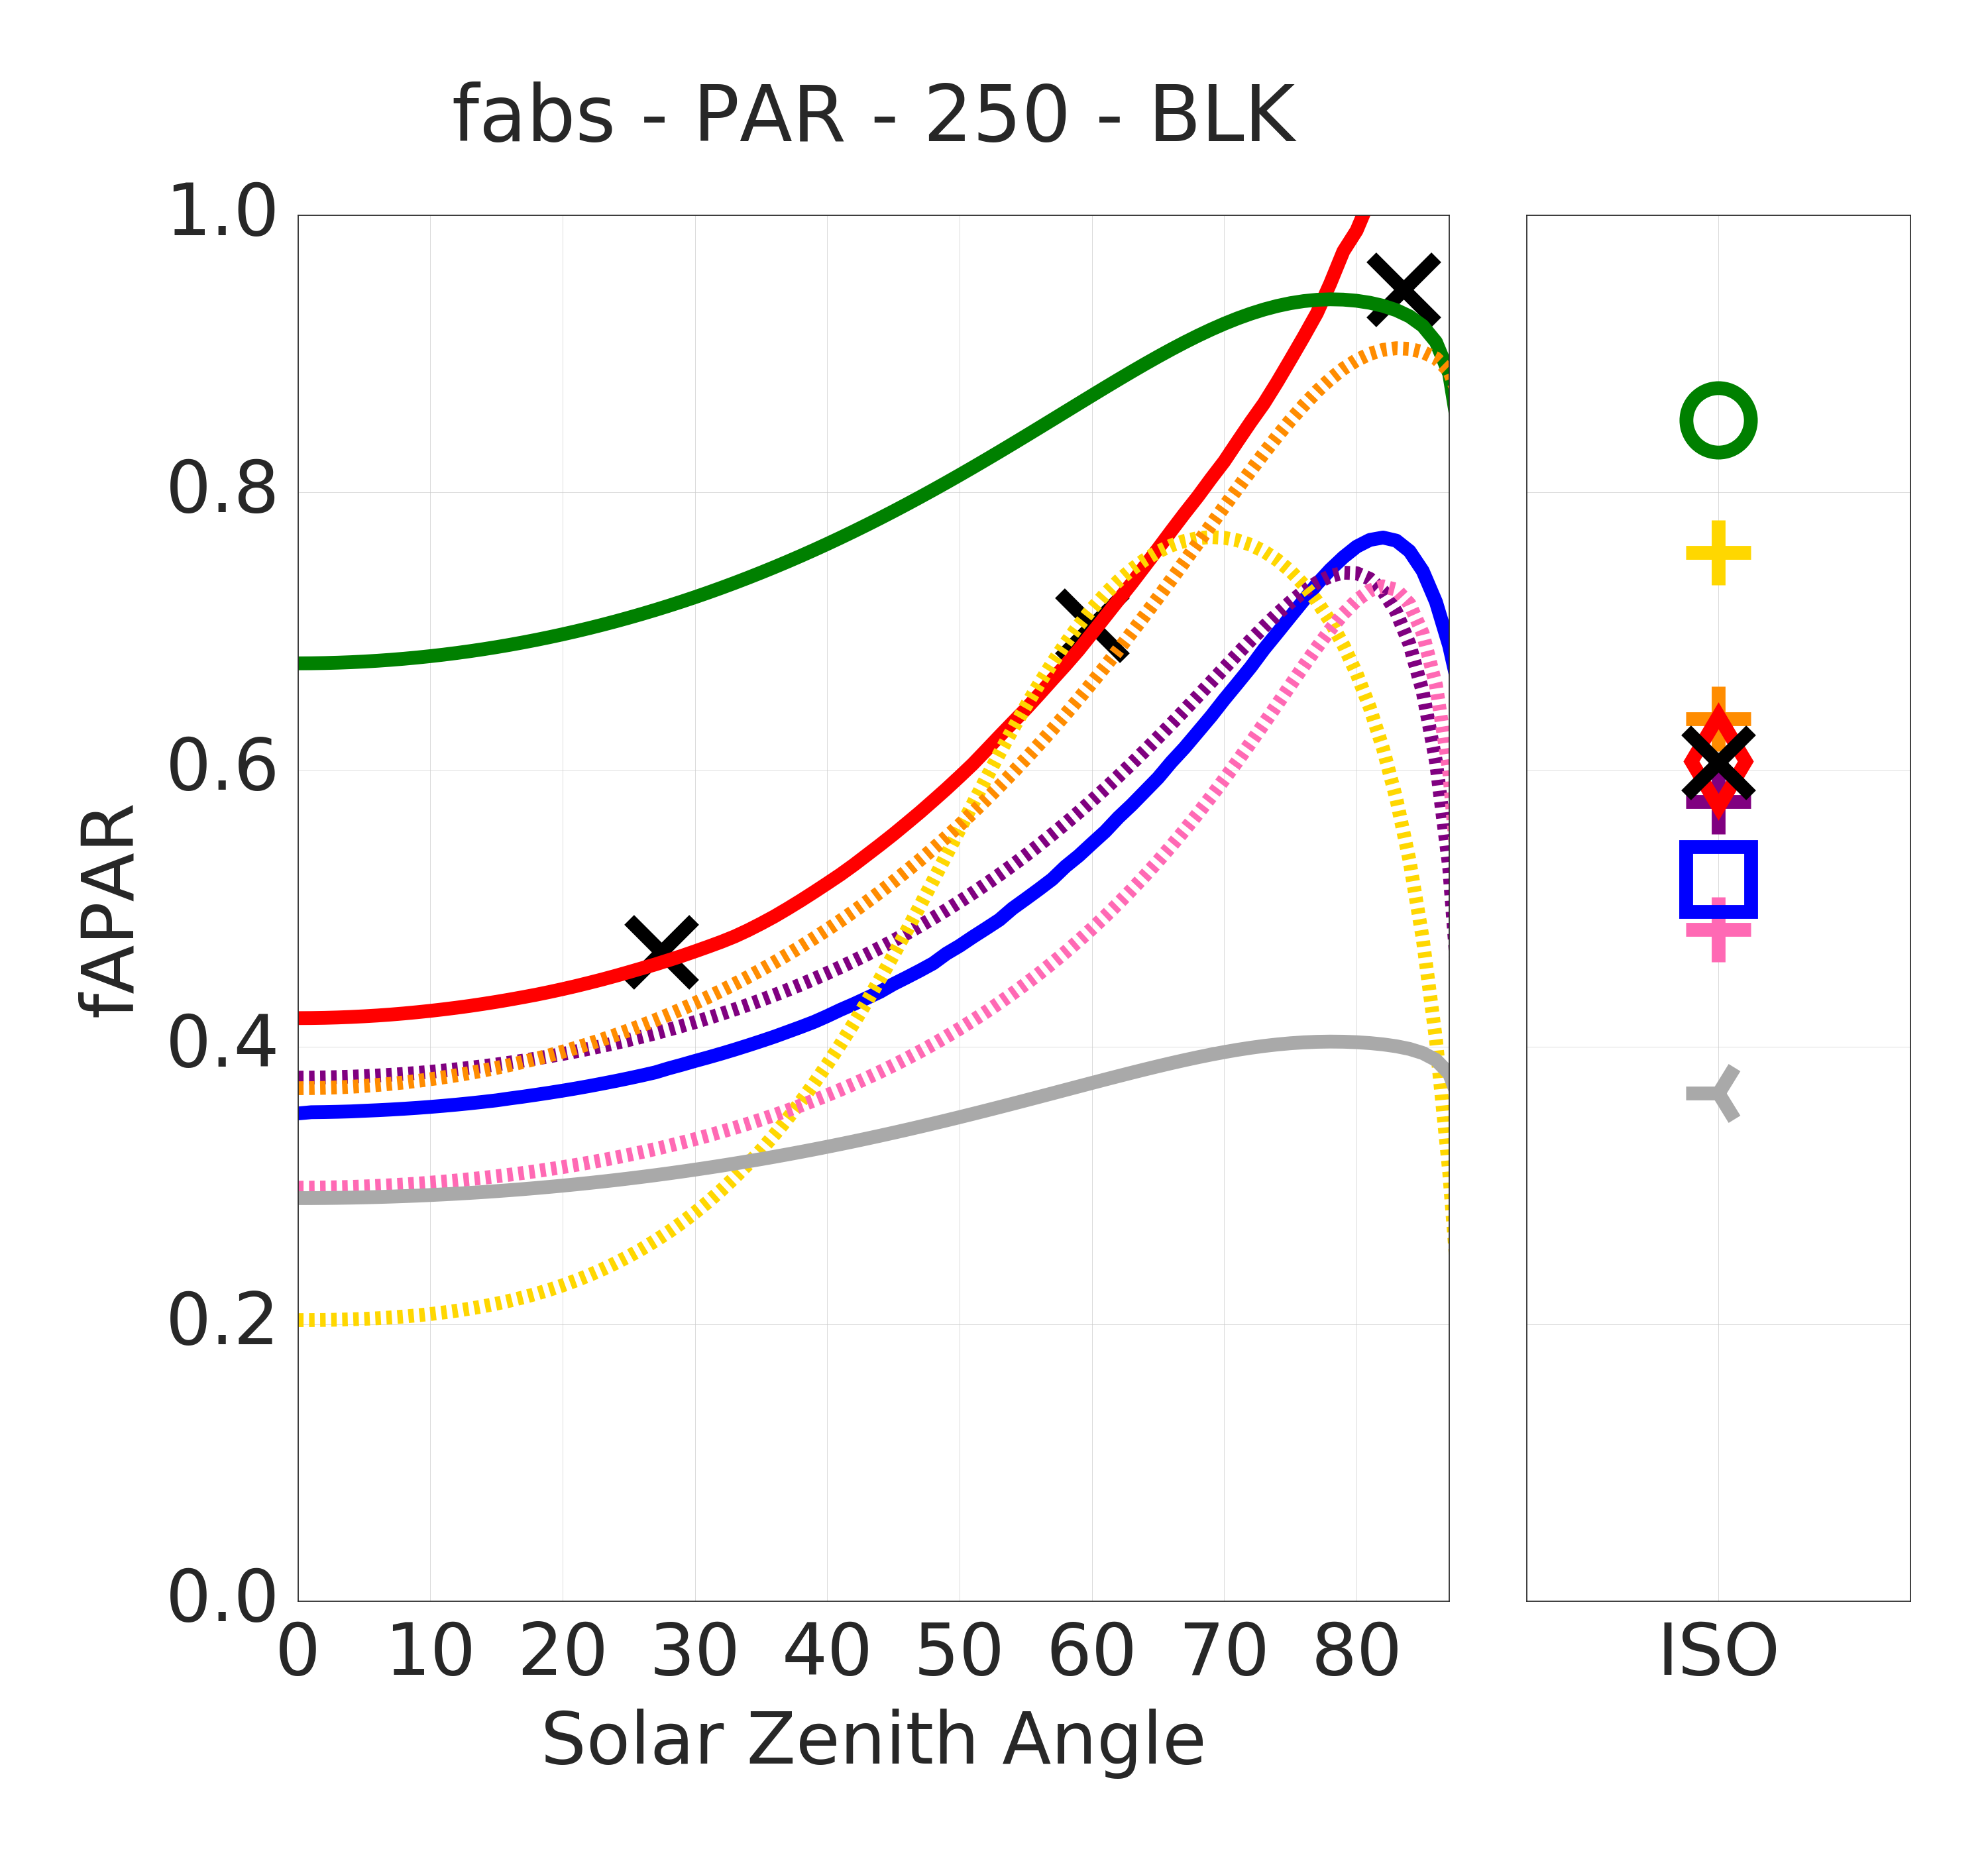
\includegraphics[width=0.33\textwidth]{/home/mn811042/src/julesRT_struct_2/julesRT_struct/data_comparison/figures/fapar_250_BLK.png}
                 %\includegraphics[width=0.33\textwidth]{/home/mn811042/src/julesRT_struct_2/julesRT_struct/JULES_STRUCT_FACTOR/fabs_PAR_250_MED_STRUC.png}
                 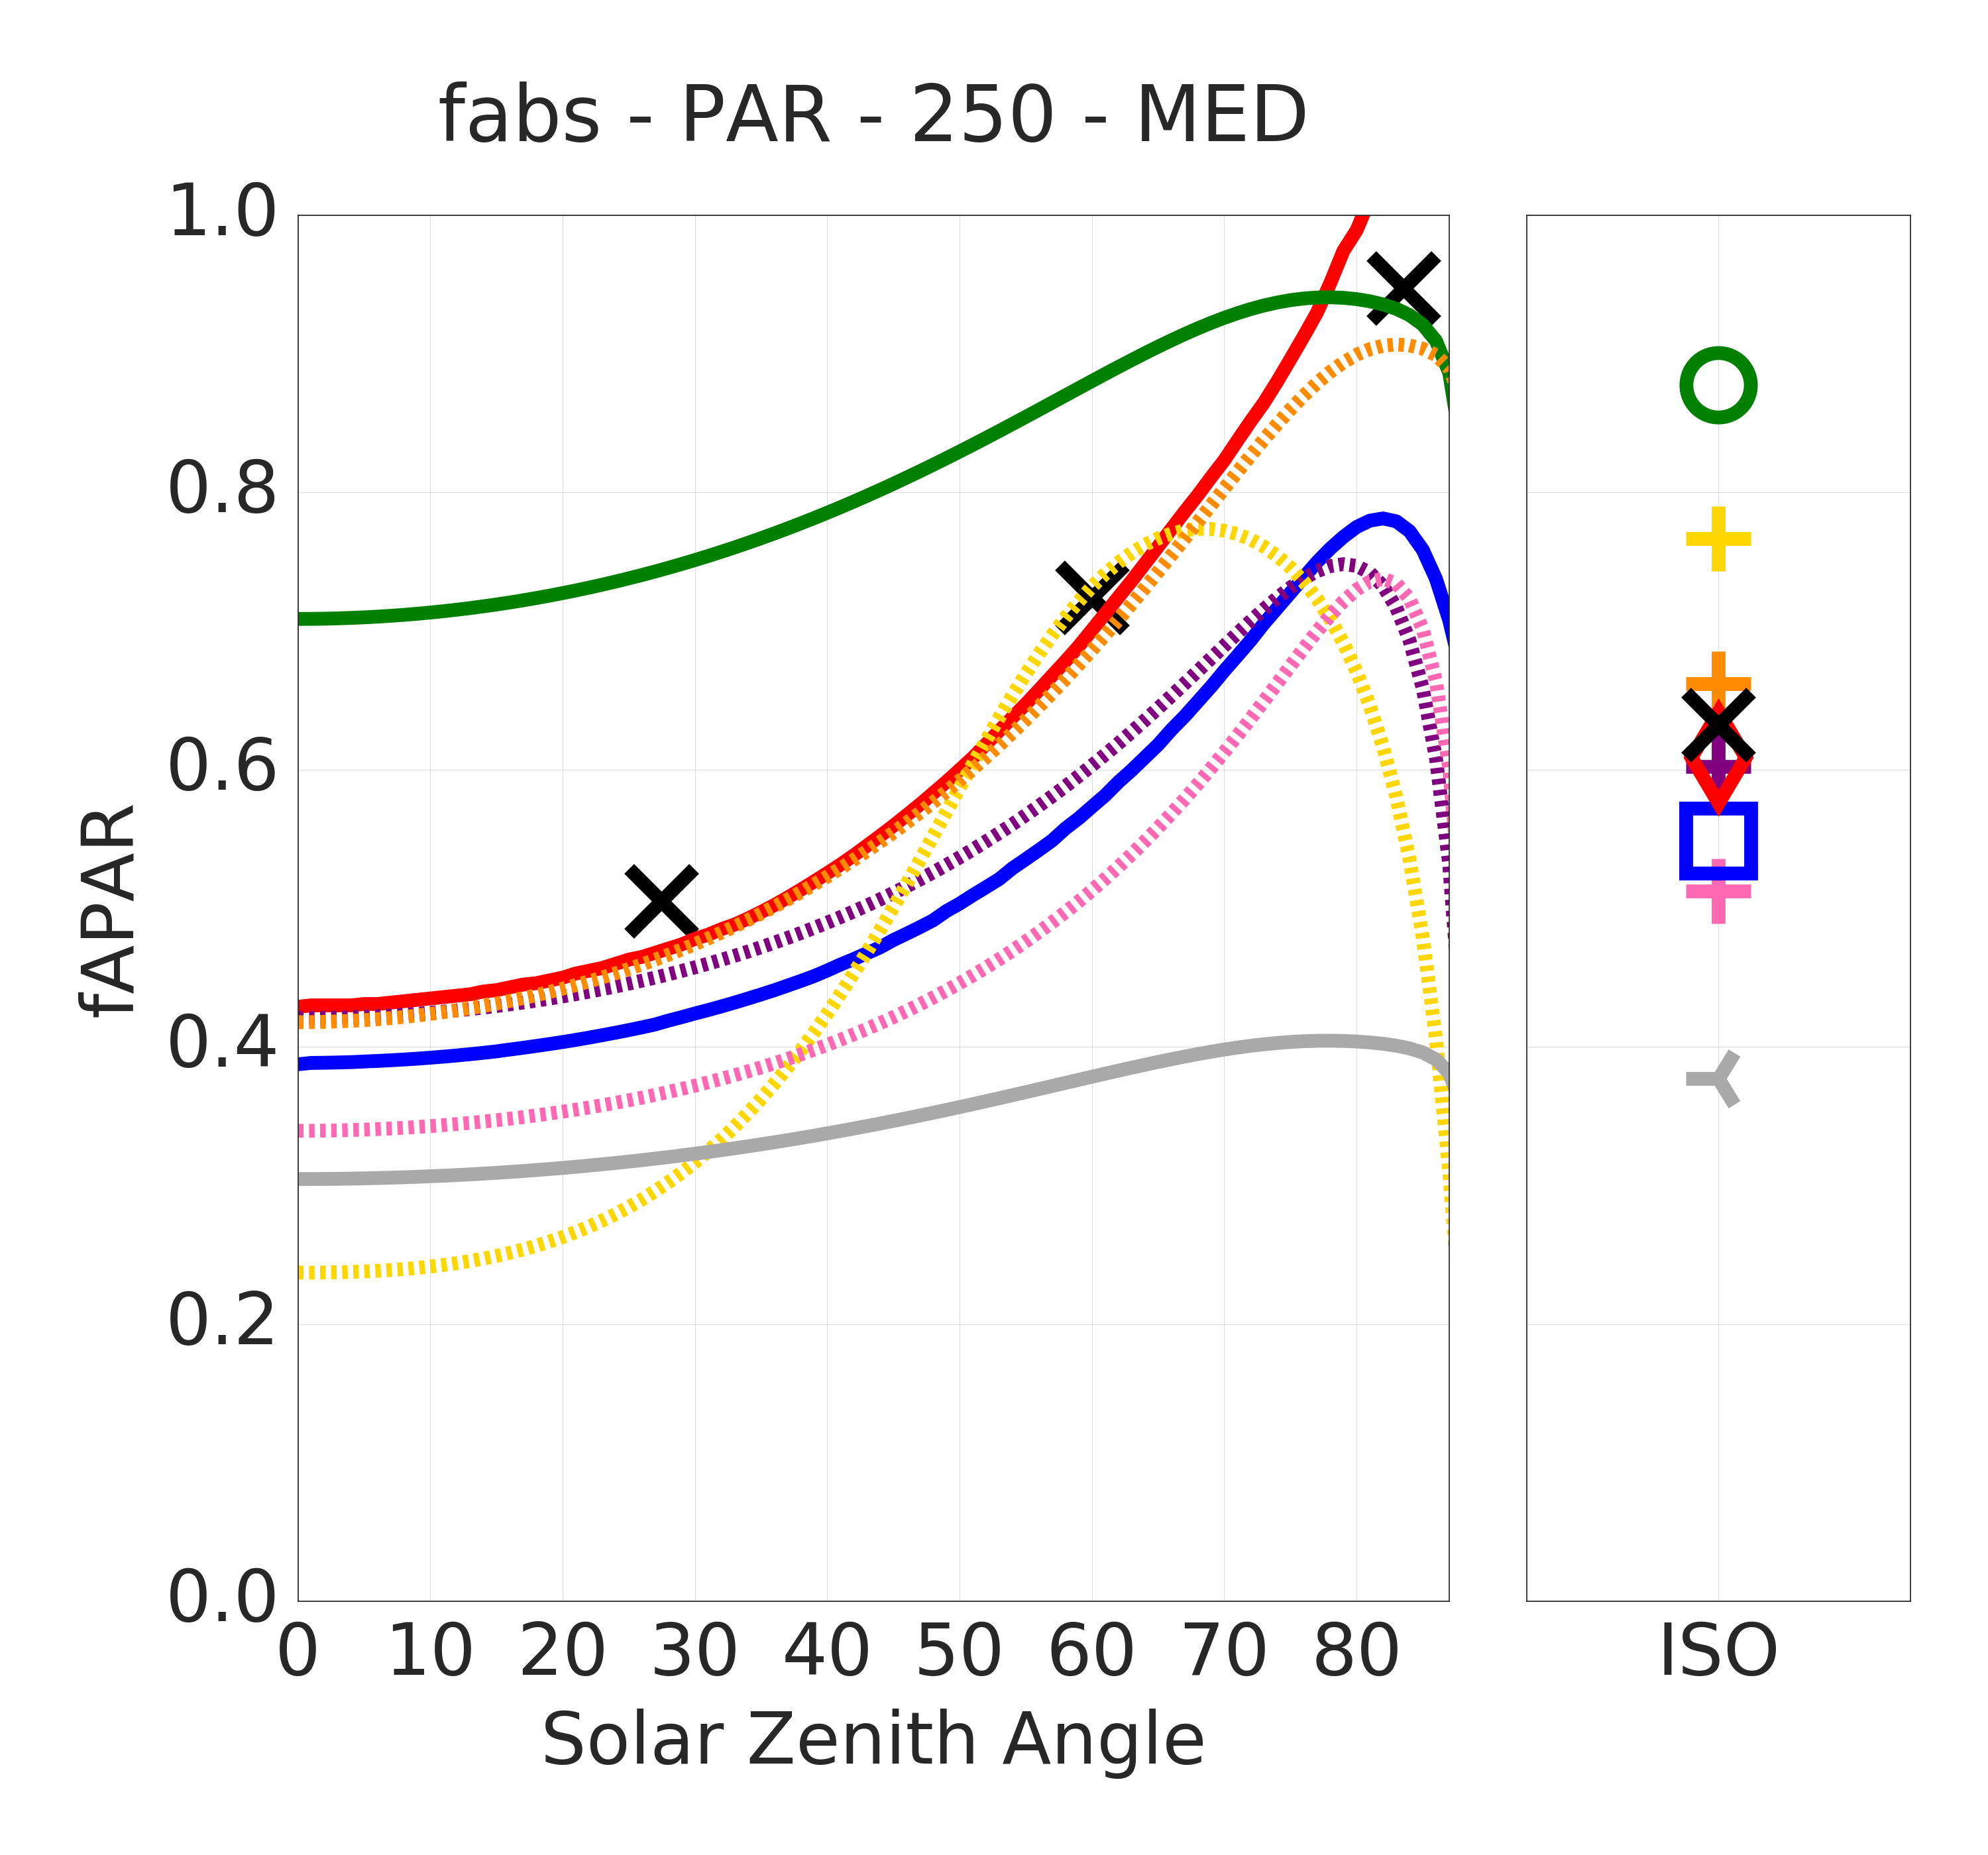
\includegraphics[width=0.33\textwidth]{/home/mn811042/src/julesRT_struct_2/julesRT_struct/data_comparison/figures/fapar_250_MED.png}
                 %\includegraphics[width=0.33\textwidth]{/home/mn811042/src/julesRT_struct_2/julesRT_struct/JULES_STRUCT_FACTOR/fabs_PAR_250_SNW_STRUC.png}}
                 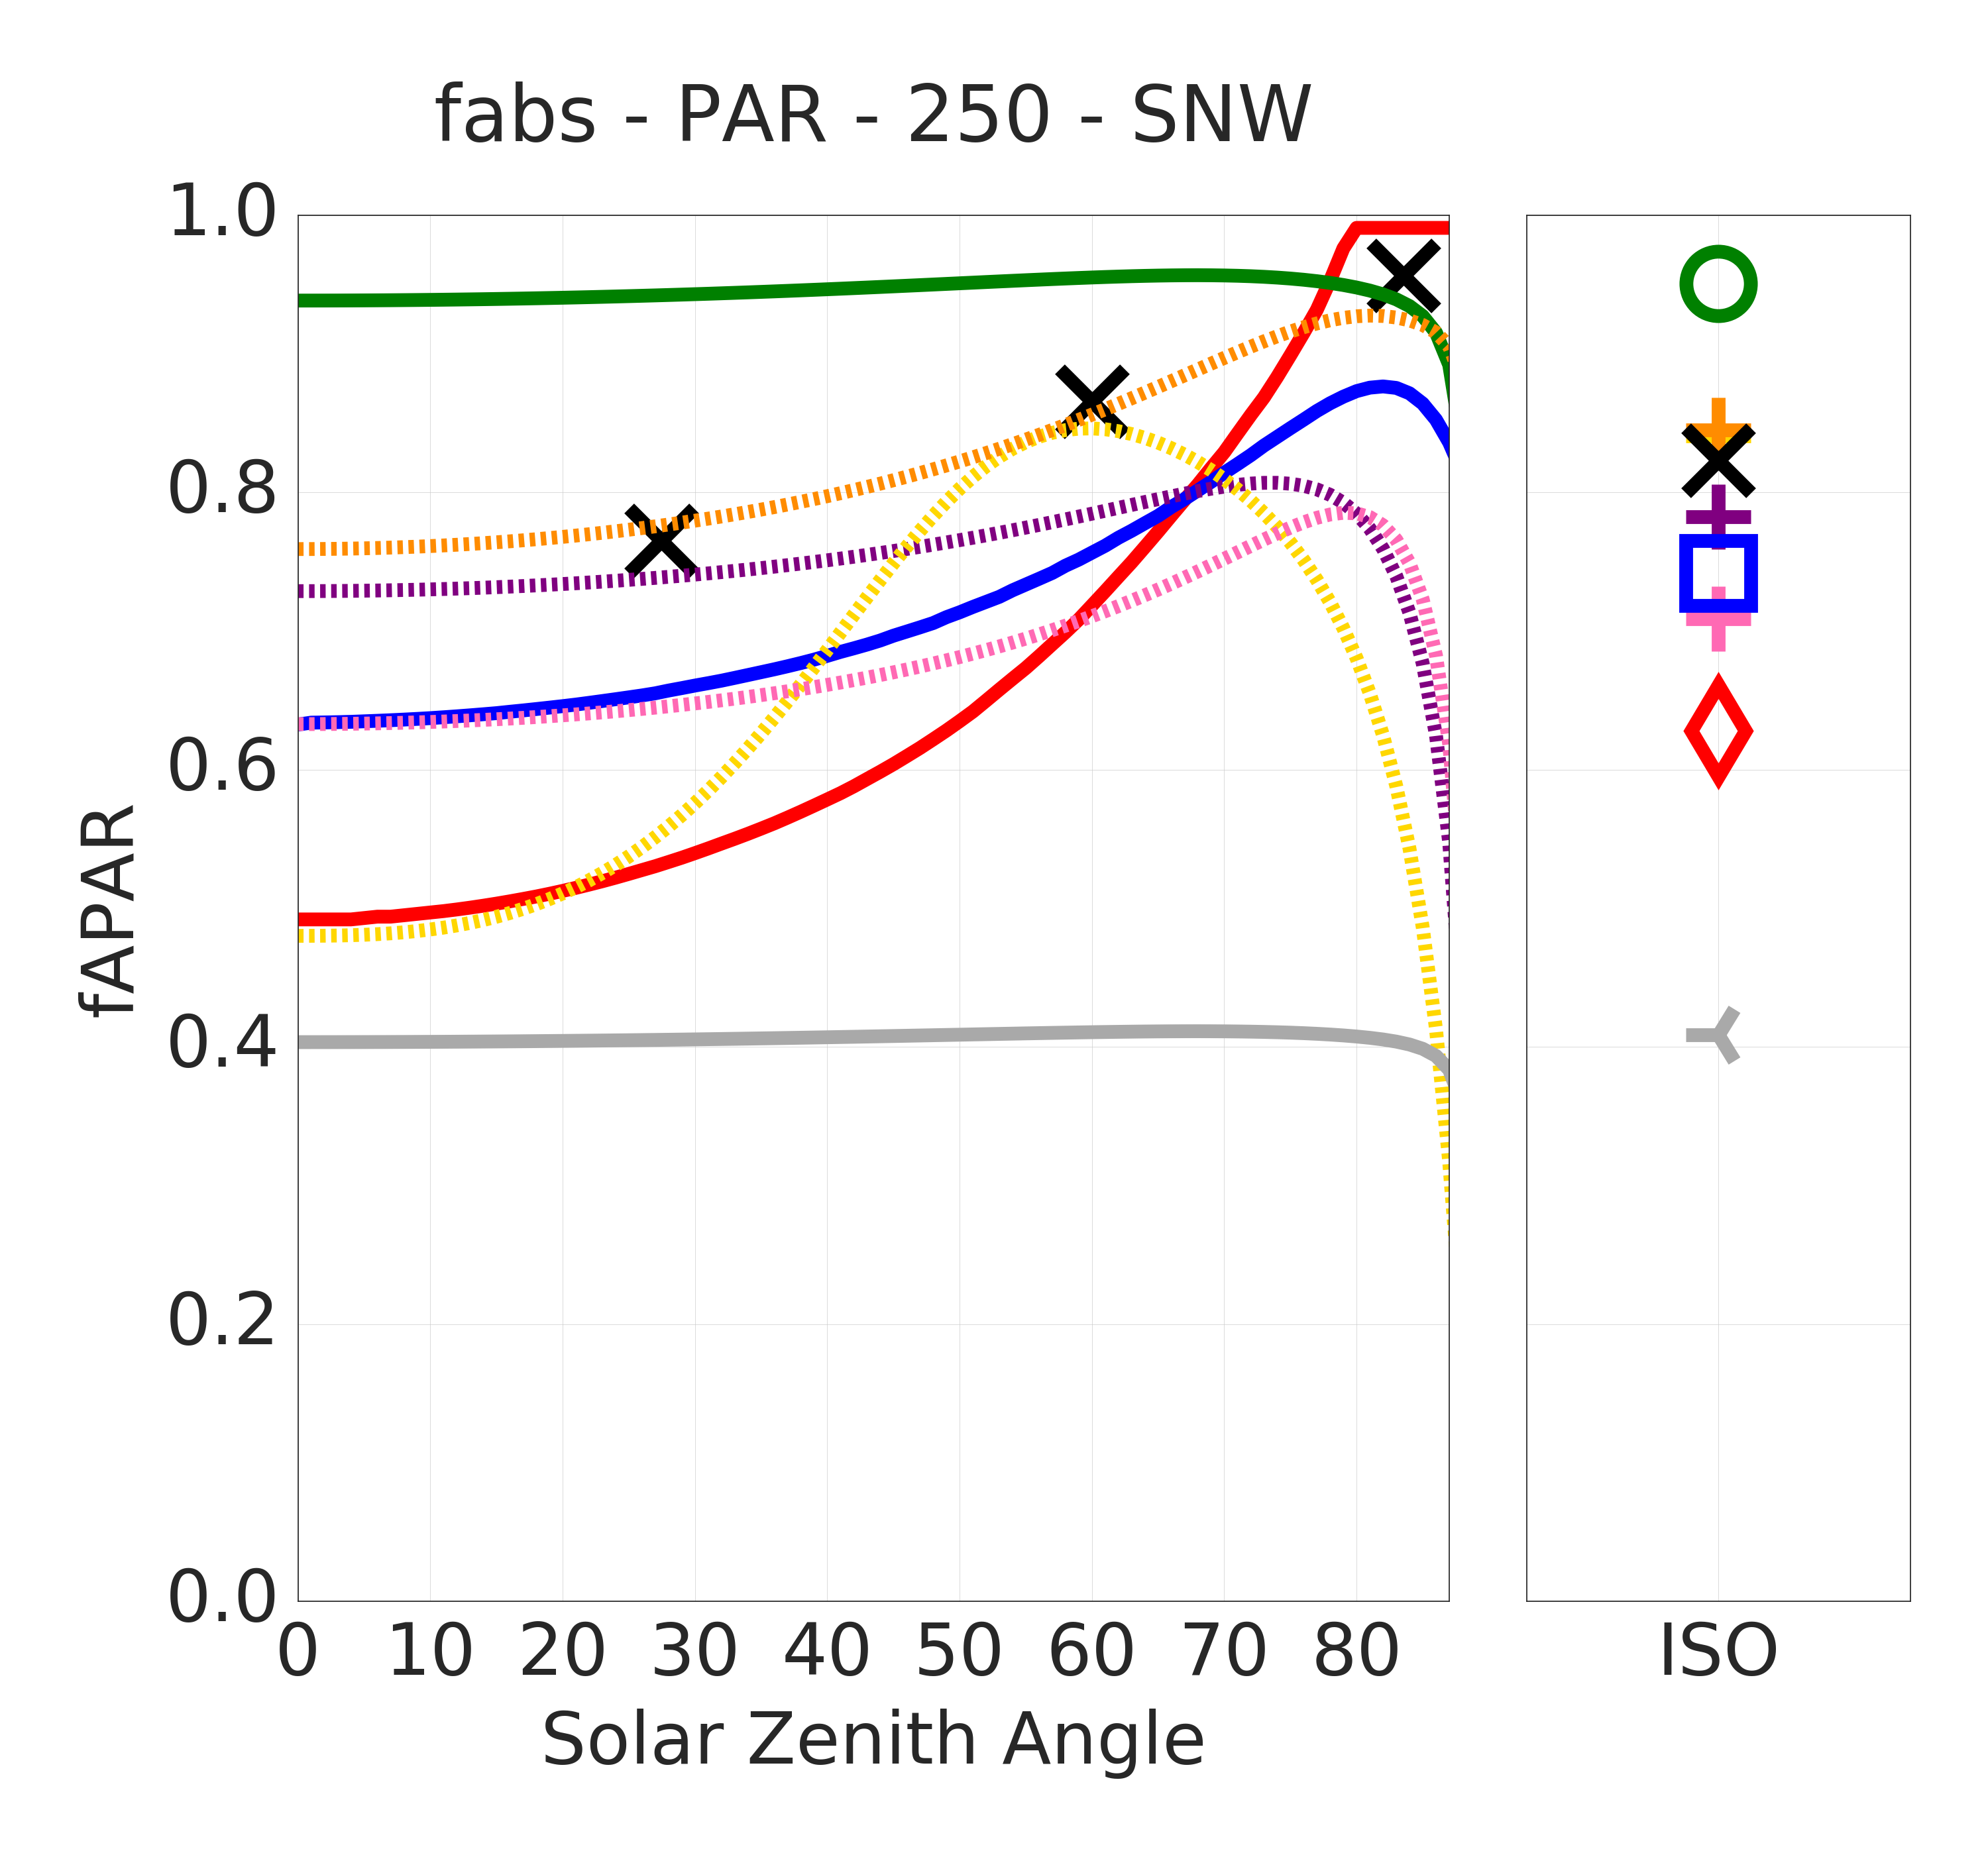
\includegraphics[width=0.33\textwidth]{/home/mn811042/src/julesRT_struct_2/julesRT_struct/data_comparison/figures/fapar_250_SNW.png}}

\end{tabular}
\caption{Intercomparison of zenith profile of fraction of direct, and diffuse (ISO) absorbed PAR (400-700 nm) calculated with 3 different models (two-stream, MAESPA, and GORT), 4 clumping indices applied into the two-stream scheme (\citet{Nilson1971}, \citet{Kucharik1999}, \citet{pinty2006}, and \citet{Ni-Meister2010}), a parameterisation scheme of the two-stream scheme commonly used in LSMs based on the vegetation cover of a gridbox (Veg$_{frac}$), and the reference values obtained with a 3D Monte Carlo ray-tracing model, raytran (RAMI4PILPS).}
\label{f:szacomparisonfPAR}
\end{figure}

\begin{figure}
%\centering
%\begin{tabular}{lll}
%\subfloat[Sparse]{\includegraphics[width=0.33\textwidth]{/home/mn811042/src/julesRT_struct_2/julesRT_struct/JULES_STRUCT_FACTOR/fabs_NIR_050_BLK_STRUC_pysellers.png}
%                  \includegraphics[width=0.33\textwidth]{/home/mn811042/src/julesRT_struct_2/julesRT_struct/JULES_STRUCT_FACTOR/fabs_NIR_050_MED_STRUC_pysellers.png}
%                  \includegraphics[width=0.33\textwidth]{/home/mn811042/src/julesRT_struct_2/julesRT_struct/JULES_STRUCT_FACTOR/fabs_NIR_050_SNW_STRUC_pysellers.png}}
%\end{tabular}
%\begin{tabular}{lll}
%\subfloat[Medium]{\includegraphics[width=0.33\textwidth]{/home/mn811042/src/julesRT_struct_2/julesRT_struct/JULES_STRUCT_FACTOR/fabs_NIR_150_BLK_STRUC_pysellers.png}
%                  \includegraphics[width=0.33\textwidth]{/home/mn811042/src/julesRT_struct_2/julesRT_struct/JULES_STRUCT_FACTOR/fabs_NIR_150_MED_STRUC_pysellers.png}
%                  %\includegraphics[width=0.33\textwidth]{/home/mn811042/src/julesRT_struct_2/julesRT_struct/JULES_STRUCT_FACTOR/fabs_NIR_150_SNW_STRUC_pysellers.png}}
%\end{tabular}
%\begin{tabular}{lll}
%\subfloat[Dense]{\includegraphics[width=0.33\textwidth]{/home/mn811042/src/julesRT_struct_2/julesRT_struct/JULES_STRUCT_FACTOR/fabs_NIR_250_BLK_STRUC_pysellers.png}
%                 \includegraphics[width=0.33\textwidth]{/home/mn811042/src/julesRT_struct_2/julesRT_struct/JULES_STRUCT_FACTOR/fabs_NIR_250_MED_STRUC_pysellers.png}
%                 \includegraphics[width=0.33\textwidth]{/home/mn811042/src/julesRT_struct_2/julesRT_struct/JULES_STRUCT_FACTOR/fabs_NIR_250_SNW_STRUC_pysellers.png}}
%\end{tabular}
\centering
\begin{tabular}{lll}
\subfloat[Sparse]{%\includegraphics[width=0.33\textwidth]{/home/mn811042/src/julesRT_struct_2/julesRT_struct/JULES_STRUCT_FACTOR/fabs_PAR_050_BLK_STRUC.png}
                  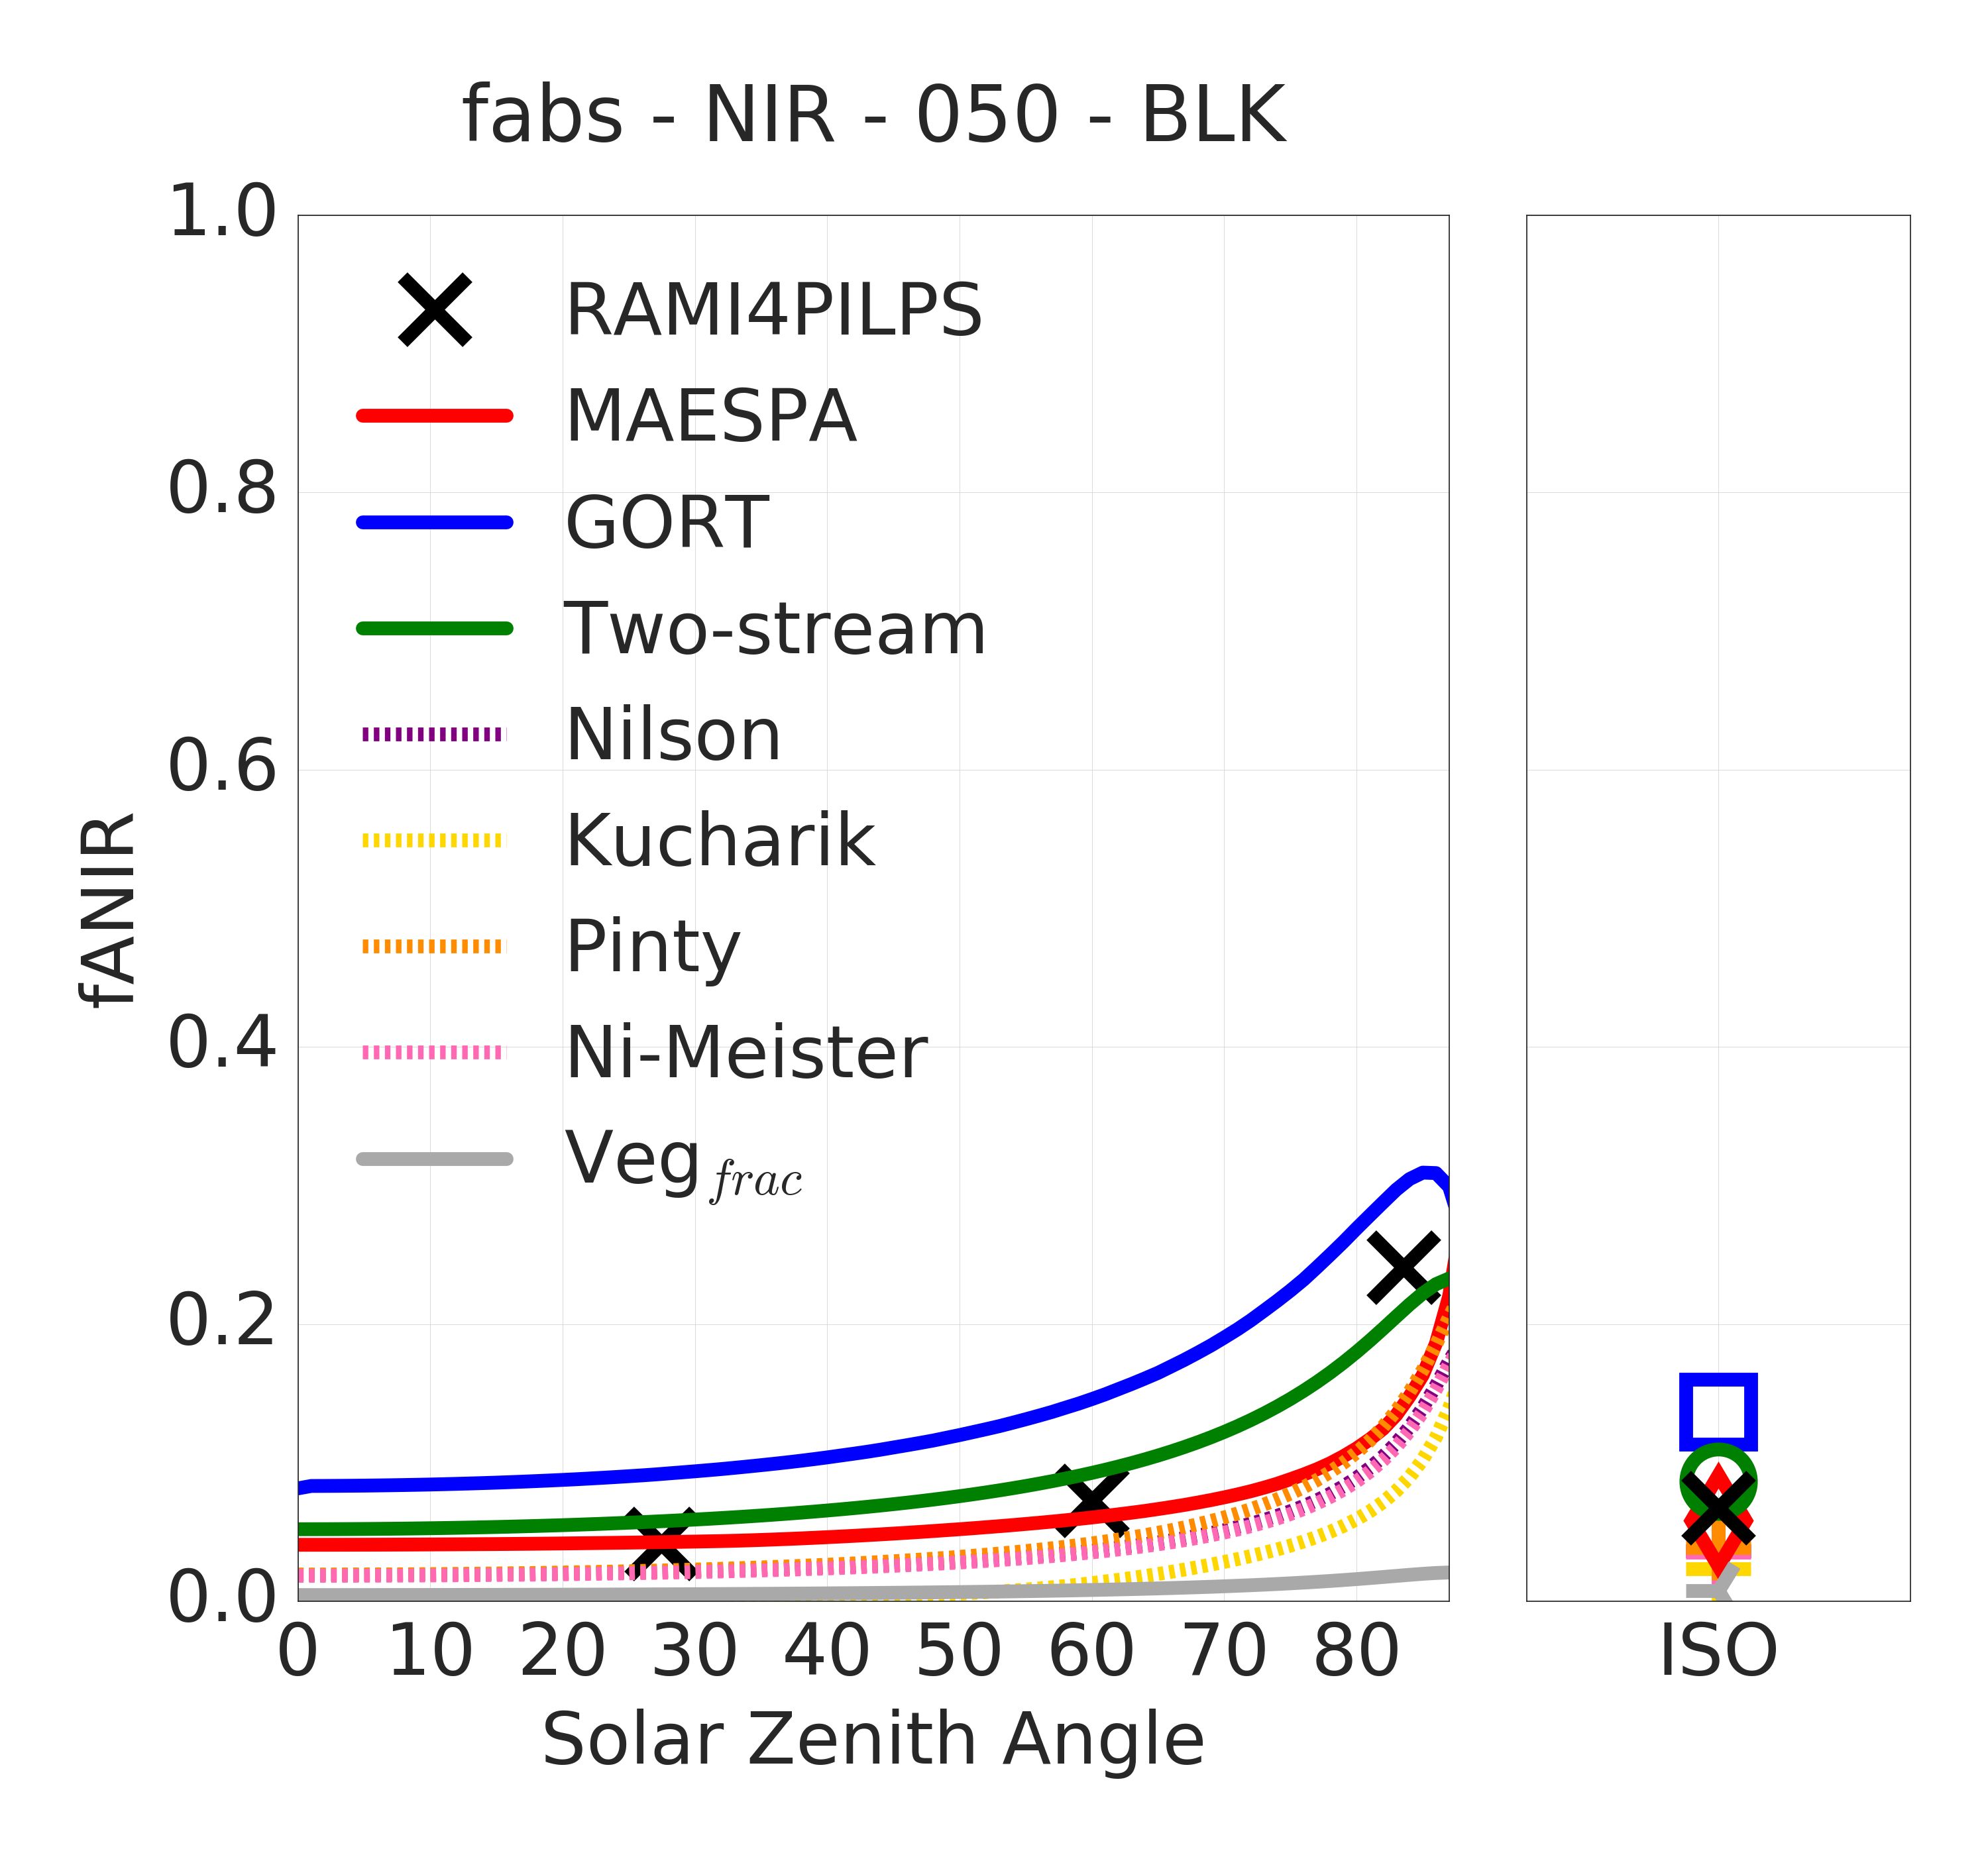
\includegraphics[width=0.33\textwidth]{/home/mn811042/src/julesRT_struct_2/julesRT_struct/data_comparison/figures/fanir_050_BLK.png}
                  %\includegraphics[width=0.33\textwidth]{/home/mn811042/src/julesRT_struct_2/julesRT_struct/JULES_STRUCT_FACTOR/fabs_PAR_050_MED_STRUC.png}
                  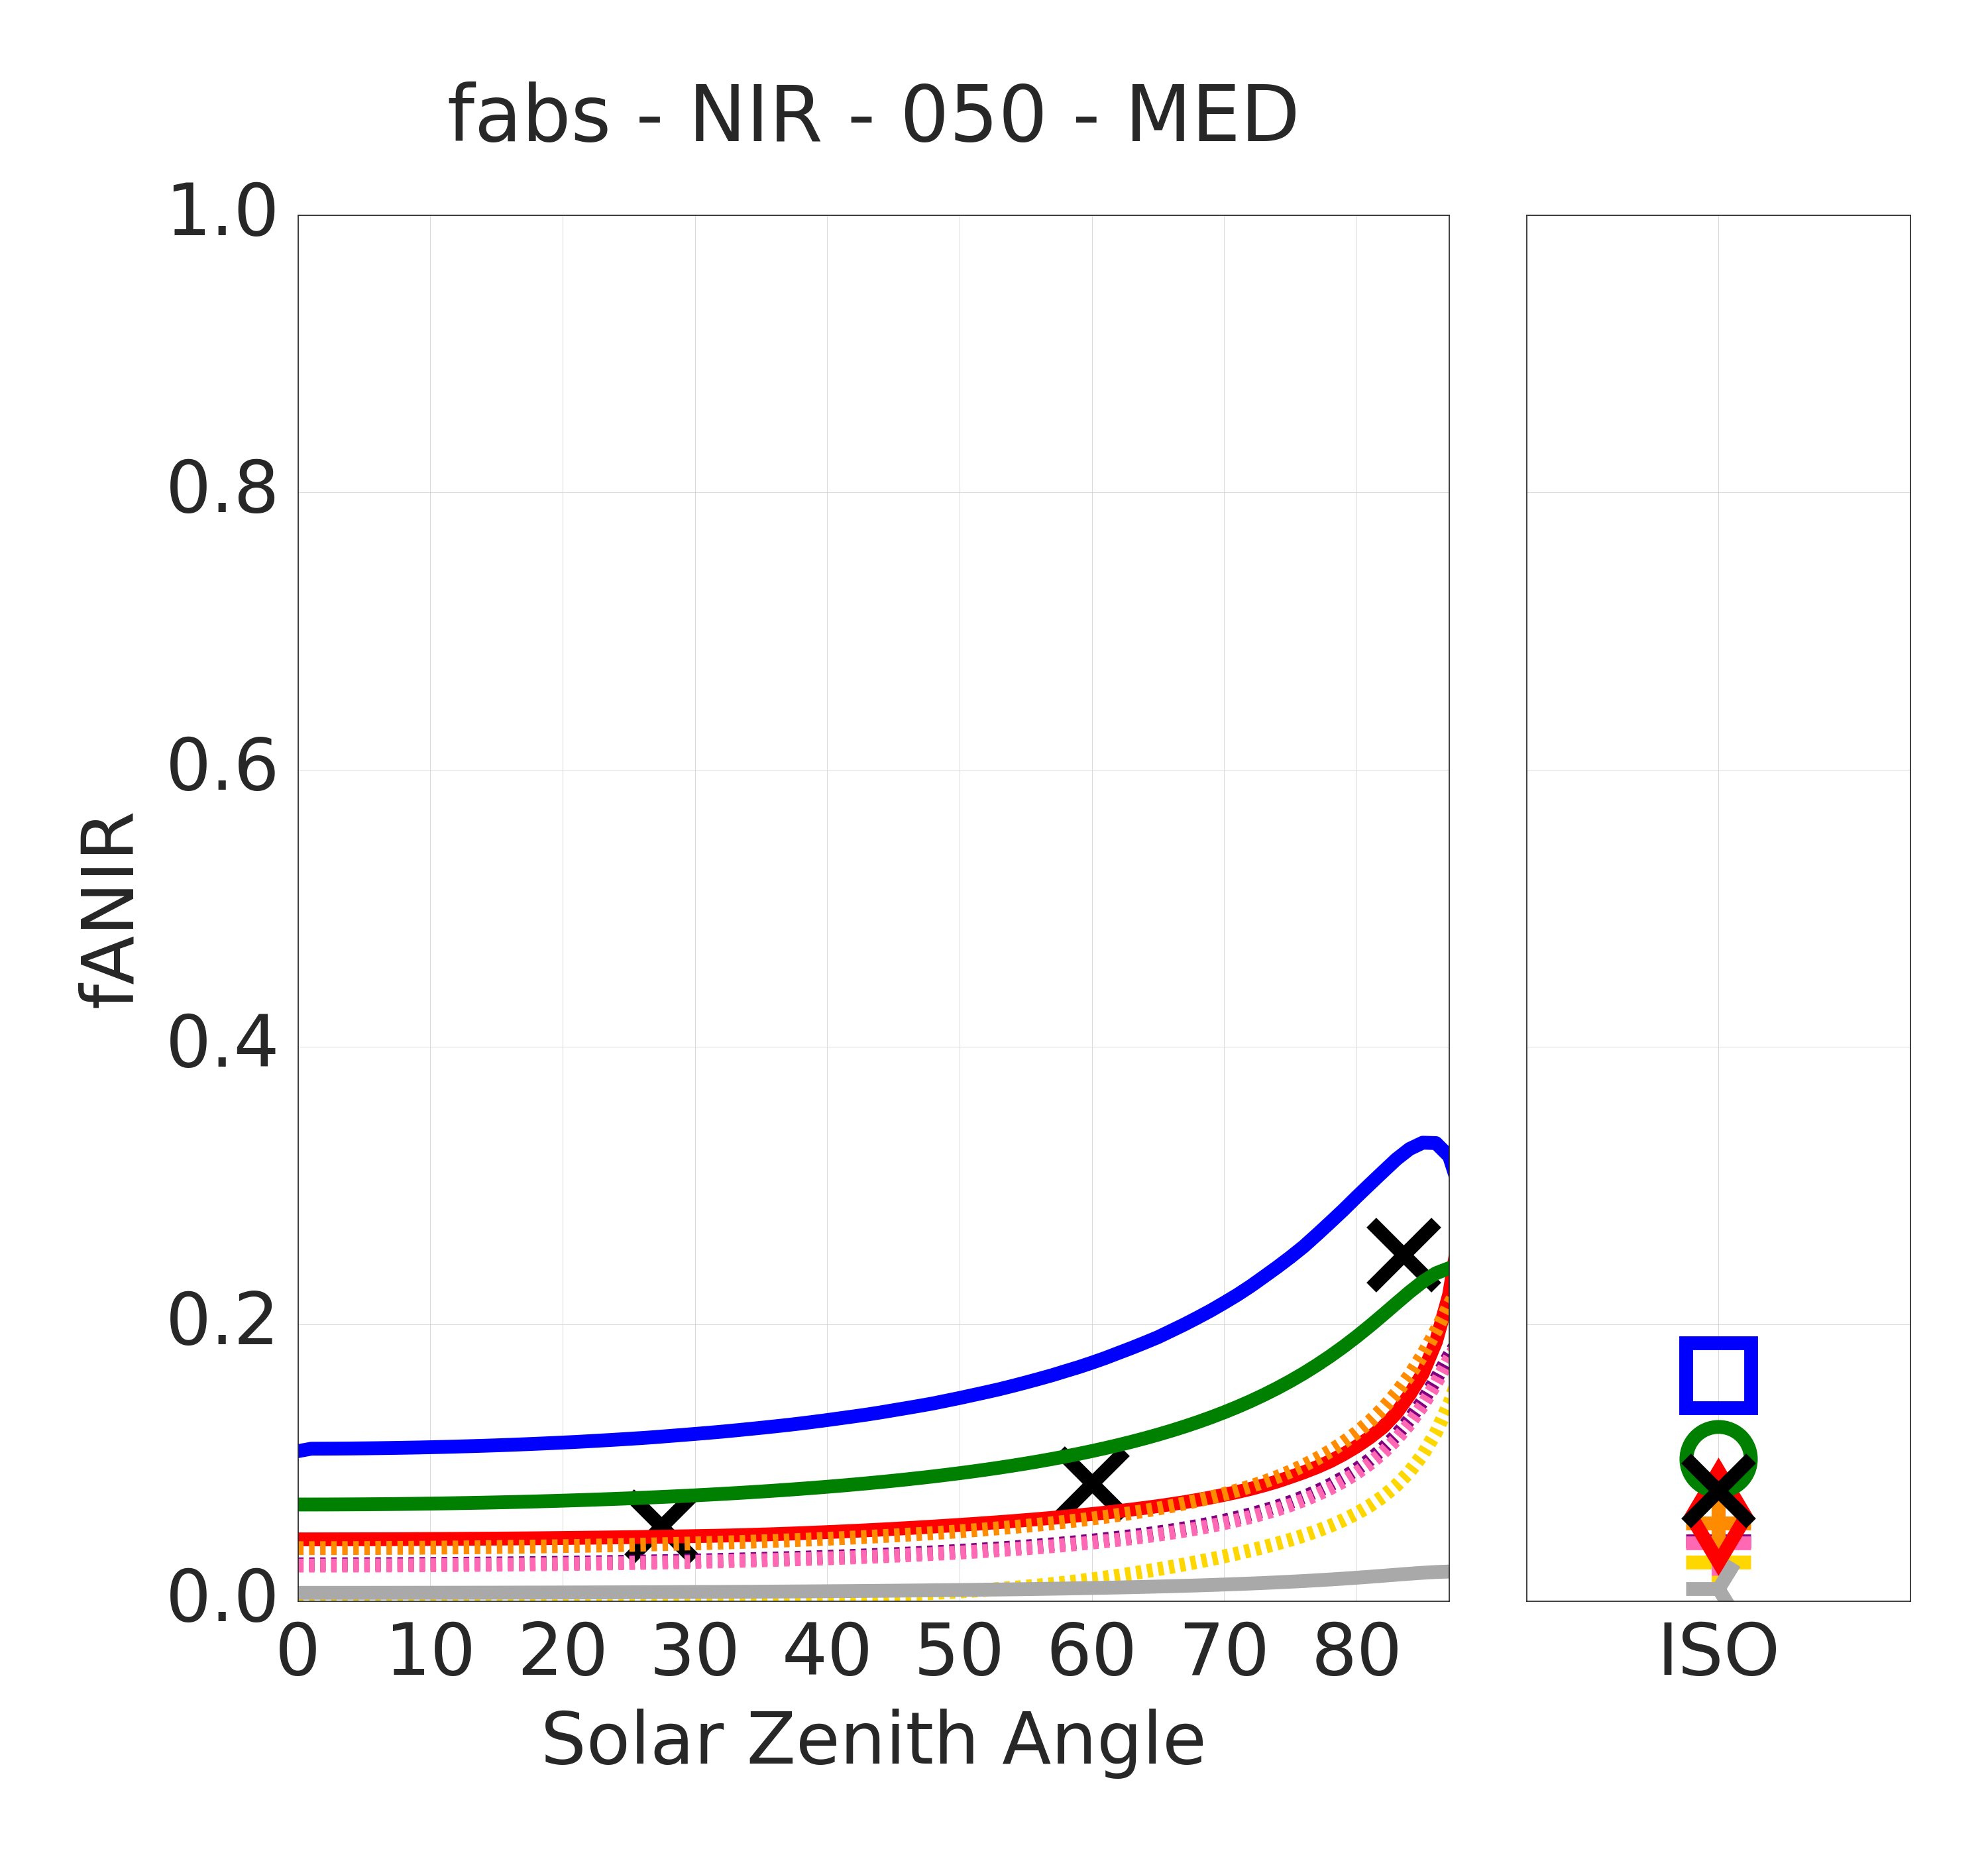
\includegraphics[width=0.33\textwidth]{/home/mn811042/src/julesRT_struct_2/julesRT_struct/data_comparison/figures/fanir_050_MED.png}
                  %\includegraphics[width=0.33\textwidth]{/home/mn811042/src/julesRT_struct_2/julesRT_struct/JULES_STRUCT_FACTOR/fabs_PAR_050_SNW_STRUC.png}}
                  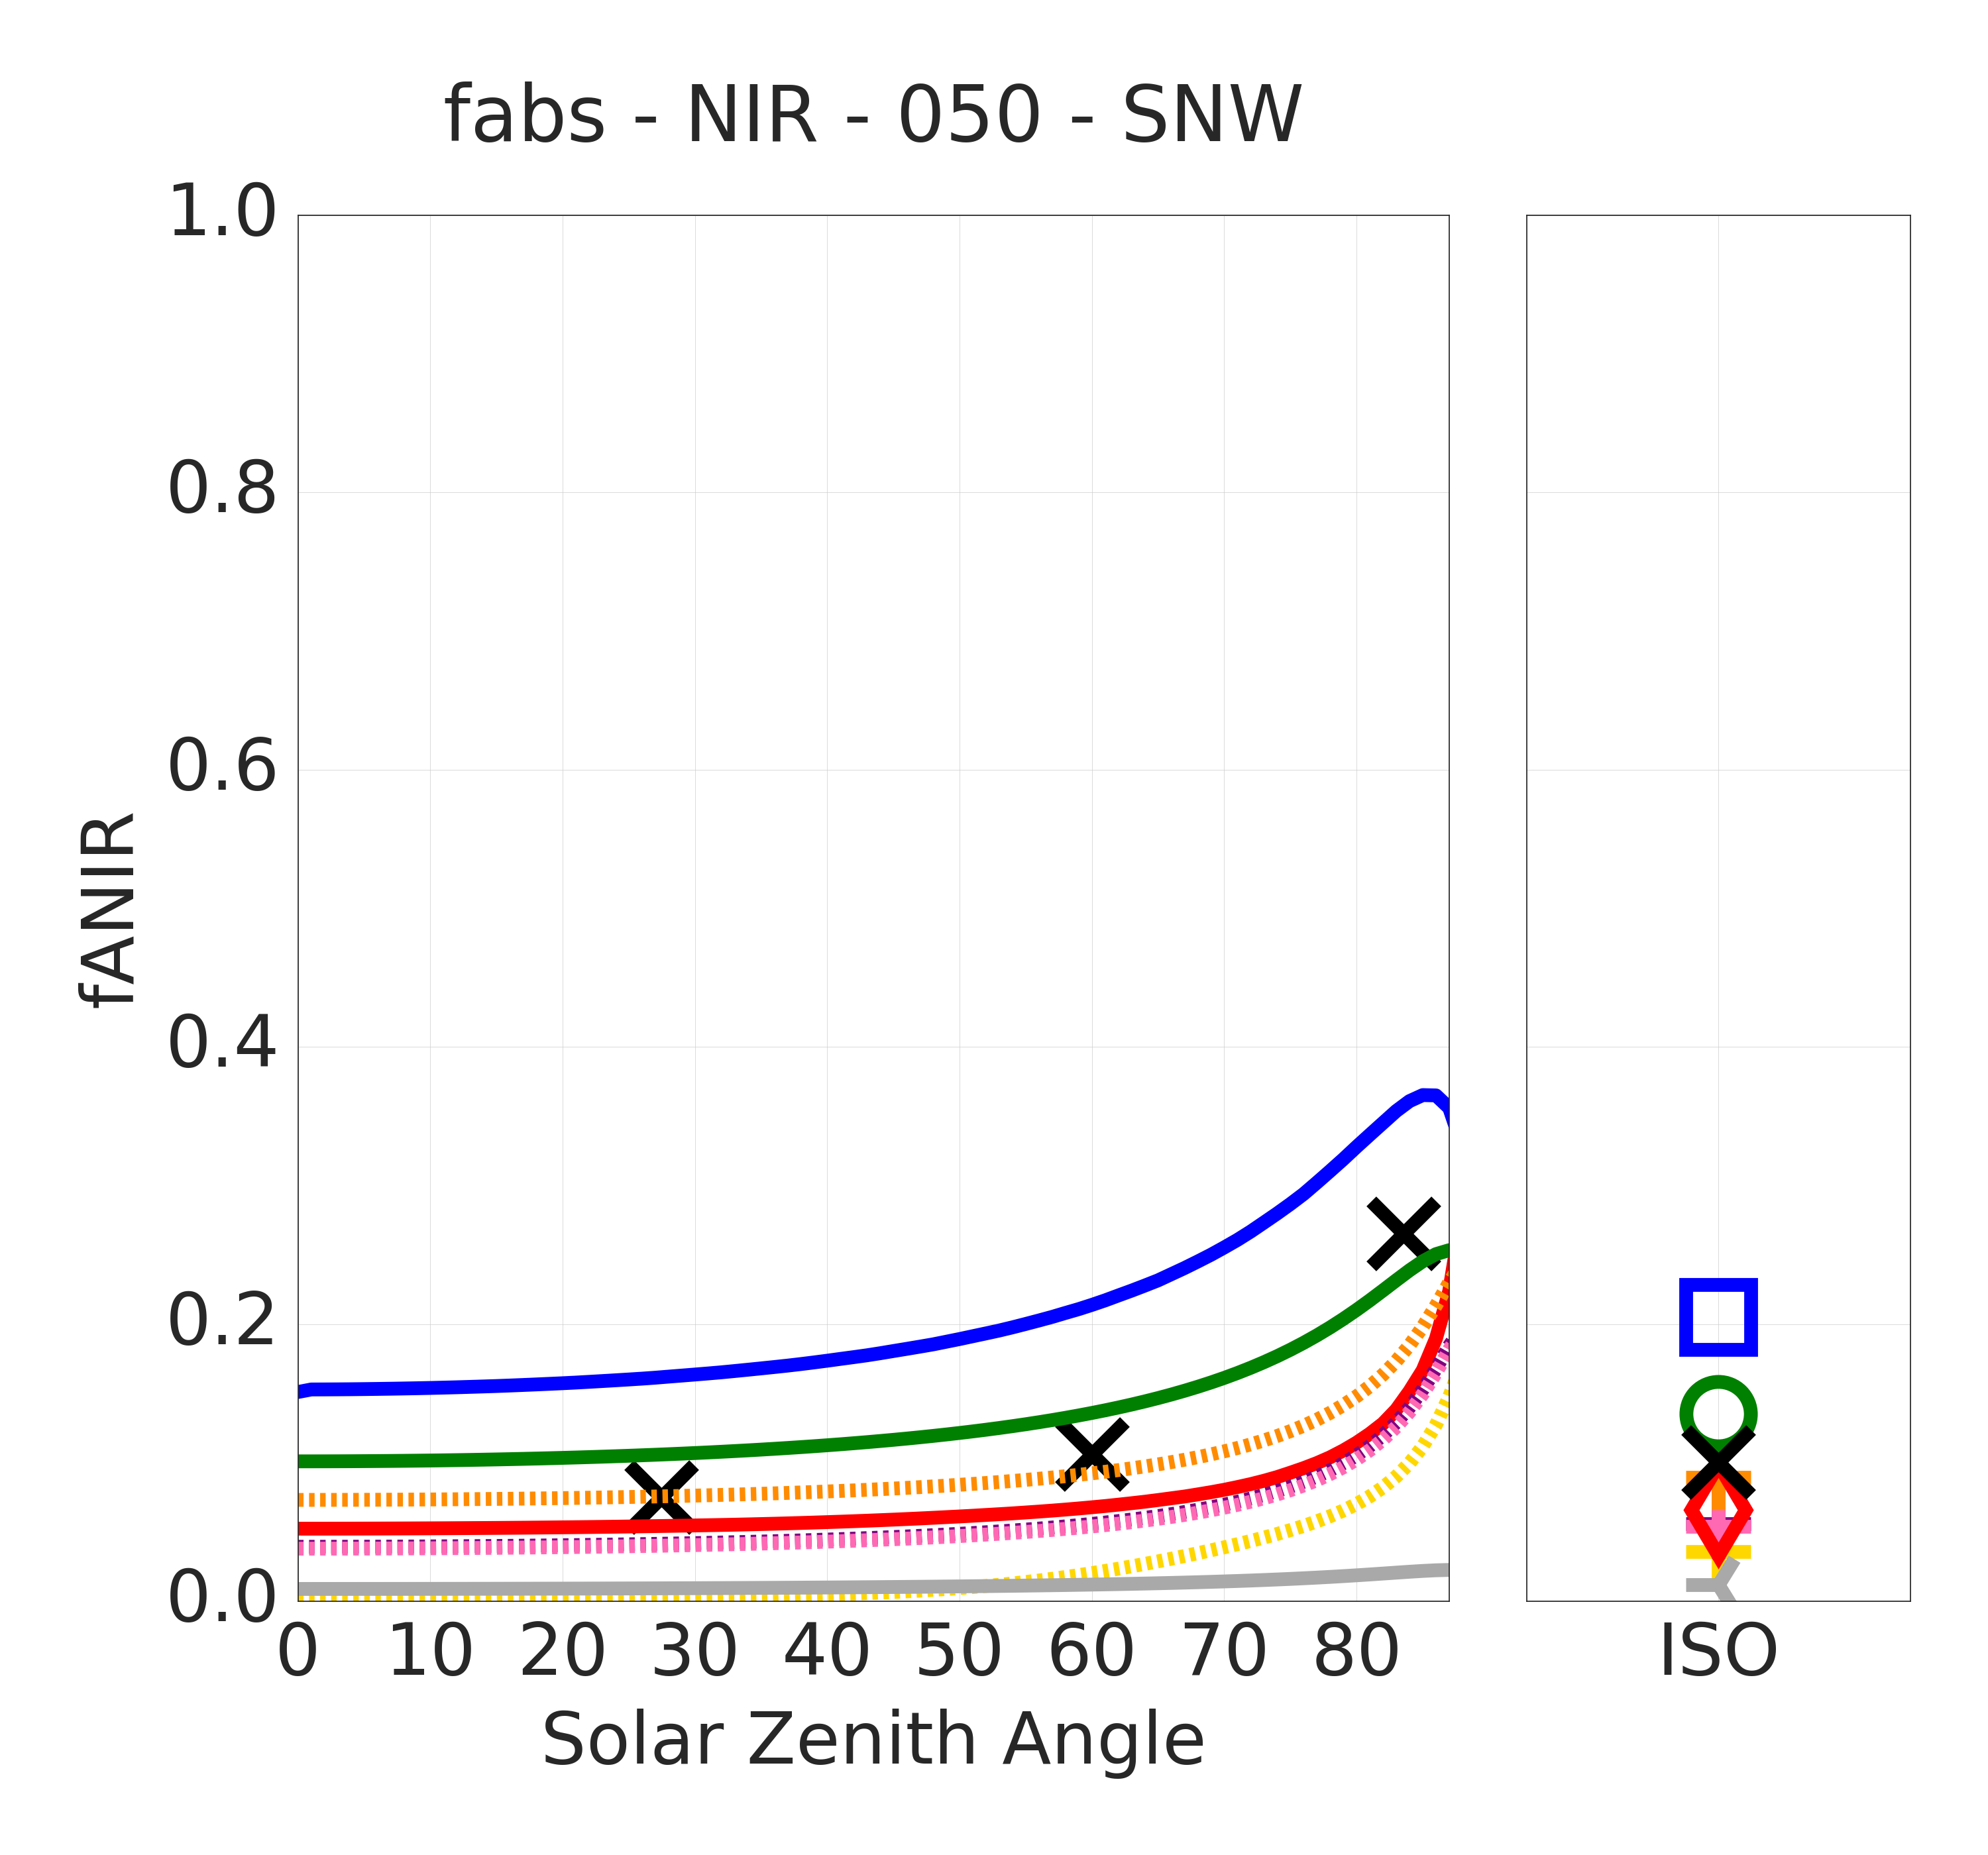
\includegraphics[width=0.33\textwidth]{/home/mn811042/src/julesRT_struct_2/julesRT_struct/data_comparison/figures/fanir_050_SNW.png}}
\end{tabular}
\begin{tabular}{lll}
\subfloat[Medium]{%\includegraphics[width=0.33\textwidth]{/home/mn811042/src/julesRT_struct_2/julesRT_struct/JULES_STRUCT_FACTOR/fabs_PAR_150_BLK_STRUC.png}
                  \includegraphics[width=0.33\textwidth]{/home/mn811042/src/julesRT_struct_2/julesRT_struct/data_comparison/figures/fanir_150_BLK.png}
                  %\includegraphics[width=0.33\textwidth]{/home/mn811042/src/julesRT_struct_2/julesRT_struct/JULES_STRUCT_FACTOR/fabs_PAR_150_MED_STRUC.png}
                  \includegraphics[width=0.33\textwidth]{/home/mn811042/src/julesRT_struct_2/julesRT_struct/data_comparison/figures/fanir_150_MED.png}
                  %\includegraphics[width=0.33\textwidth]{/home/mn811042/src/julesRT_struct_2/julesRT_struct/JULES_STRUCT_FACTOR/fabs_PAR_150_SNW_STRUC.png}} 
                  \includegraphics[width=0.33\textwidth]{/home/mn811042/src/julesRT_struct_2/julesRT_struct/data_comparison/figures/fanir_150_SNW.png}}
\end{tabular}
\begin{tabular}{lll}
\subfloat[Dense]{%\includegraphics[width=0.33\textwidth]{/home/mn811042/src/julesRT_struct_2/julesRT_struct/JULES_STRUCT_FACTOR/fabs_PAR_250_BLK_STRUC.png}
                 \includegraphics[width=0.33\textwidth]{/home/mn811042/src/julesRT_struct_2/julesRT_struct/data_comparison/figures/fanir_250_BLK.png}
                 %\includegraphics[width=0.33\textwidth]{/home/mn811042/src/julesRT_struct_2/julesRT_struct/JULES_STRUCT_FACTOR/fabs_PAR_250_MED_STRUC.png}
                 \includegraphics[width=0.33\textwidth]{/home/mn811042/src/julesRT_struct_2/julesRT_struct/data_comparison/figures/fanir_250_MED.png}
                 %\includegraphics[width=0.33\textwidth]{/home/mn811042/src/julesRT_struct_2/julesRT_struct/JULES_STRUCT_FACTOR/fabs_PAR_250_SNW_STRUC.png}}
                 \includegraphics[width=0.33\textwidth]{/home/mn811042/src/julesRT_struct_2/julesRT_struct/data_comparison/figures/fanir_250_SNW.png}}

\end{tabular}
\caption{Intercomparison of zenith profile of fraction of direct, and diffuse (ISO) absorbed NIR (700-3000 nm) calculated with 3 different models (two-stream, MAESPA, and GORT), 4 clumping indices applied into the two-stream scheme (\citet{Nilson1971}, \citet{Kucharik1999}, \citet{pinty2006}, and \citet{Ni-Meister2010}), a parameterisation scheme of the two-stream scheme commonly used in LSMs based on the vegetation cover of a gridbox (Veg$_{frac}$), and the reference values obtained with a 3D Monte Carlo ray-tracing model, raytran (RAMI4PILPS).}
\label{f:szacomparisonfNIR}
\end{figure}

\subsection{Reflectance}

For PAR reflectance, the two-stream scheme underestimates the reference values over the majority of the evaluated canopy densities, under both illumination conditions as well, except over black soil albedo. In this particular case, the two-stream scheme reflects more PAR radiation from the plant elements, because it does not interact with the underneath black soil as much as the 3D models, mainly because the other models take structural canopy variability into account. Moreover, the two-stream scheme is not able to obtain the correct decaying shape of reflectance with zenith angle over most of the scenes.

For canopy reflectance in the NIR spectral region, the two-stream scheme tends to overestimate the reference values over the black and medium soil albedos; but it shows a relative good agreement over a highly reflective soil (snow).

In terms of reflectance, MAESPA does not show as good agreement as for absorption with the reference values. Over black soil, MAESPA overestimates PAR reflectance for all evaluated cases, especially over the sparse case.

Over medium reflective soil, MAESPA behaves closely to the two-stream scheme over the medium, and dense canopies, but it shows opposite behaviour than all the other radiative approaches over the sparse case; i.e., PAR reflectance decreases with Sun zenith angle, while in MAESPA, canopy PAR albedo increases with solar zenith angle. 

Over snow (SNW), MAESPA underestimates PAR canopy albedo over all evaluated scenarios. MAESPA is not able to reproduce the behaviour of PAR canopy albedo with Sun zenith angle either. MAESPA does not deal with soil reflectance in an accurate manner. This result was already highlighted by its behaviour over a highly reflective soil when looking at with absorption. 

For PAR reflectance, GORT underestimates the reference values over black soil for all the evaluated canopy densities. For the medium soil albedo, GORT seemed to be the model which most agreed with the reference values, especially over the medium canopy. GORT was able to characterise exactly the decay of PAR reflectance following solar zenith angles. Over snow, GORT tends to overestimate PAR reflectance, especially over the dense canopy. In the NIR spectrum, GORT presented a persistent underestimation in reflectance, for both illumination conditions. Also, GORT was not able to reproduce the increasing curve of NIR reflectance in all evaluated cases.

The $Veg_{frac}$ correction slightly underestimates PAR, and NIR reflectances over a black soil for all canopy densities, but it is not able to reproduce the reference values for large Sun zenith angles (83.5$^{\circ}$). For a medium reflective soil background, this parameterisation scheme overestimates canopy albedo in up to 5\% over a dense canopy associated with large Sun zenith angle. Over snow, its overestimation can be up to 40\% over a dense canopy in the PAR spectral region.
For the NIR spectrum, the $Veg_{frac}$ correction shows a good agreement with the reference values for a medium reflective soil background, but underestimates it for a black soil, and overestimates it over snow.

As for PAR absorption, Pinty\textquotesingle s and Nilson\textquotesingle s clumping indices showed a very good agreement with the RAMI4PILPS reference values for PAR reflectance over snow. Their major differences are associated to the medium canopy density over snow, where the presence of the term $b$ in the structure factor (Eq.~\ref{equation:structurefactor}) seems to marginally better represent the RAMI4PILPS reference values. Followed by Ni-Meister\textquotesingle s clumping index parameterisation scheme, which was able to reproduce the curvature of PAR reflectance with zenith angle, with slightly larger overestimation than the reference values.

Figures~\ref{f:szacomparisonalbPAR} indicates that overall, the structure factor parameterisation scheme consistently showed a better agreement with the RAMI4PILPS reference values than any other approach under direct (Solar Zenith Angles from 0 to 90$^{\circ}$), and diffuse illumination conditions. It seemed to be an efficient, and accurate tool to derive PAR reflectance as well, for all evaluated scenarios, with especial attention to its performance over snow.

This effect is particularly relevant for the radiative partitioning treatment in boreal regions in the presence of snow, where the shadowing induced by sparse distributed plant structure diminishes surface albedo, in comparison to a closed-canopy/bare-snow scenario of identical cover fractions \citep{Viterbo1999}. 

In the NIR spectrum, the structure factor improves the agreement between the two-Stream scheme and the RAMI4PILPS reference values, in the sparse canopy, for reflectance, but has the opposite effect over the other canopy densities.

Besides differences between Pinty\textquotesingle s and Nilson\textquotesingle s indices, their differences were marginal if compared to other schemes. Kucharik\textquotesingle s scheme presented a more oscillating behaviour than any other method, but agreed quite well with the reference values over 60$^{\circ}$. 

\begin{figure}
%\centering
%\begin{tabular}{lll}
%\subfloat[Sparse]{\includegraphics[width=0.33\textwidth]{/home/mn811042/src/julesRT_struct_2/julesRT_struct/JULES_STRUCT_FACTOR/fref_PAR_050_BLK_STRUC.png}
%                  \includegraphics[width=0.33\textwidth]{/home/mn811042/src/julesRT_struct_2/julesRT_struct/JULES_STRUCT_FACTOR/fref_PAR_050_MED_STRUC.png}
%                  \includegraphics[width=0.33\textwidth]{/home/mn811042/src/julesRT_struct_2/julesRT_struct/JULES_STRUCT_FACTOR/fref_PAR_050_SNW_STRUC.png}}
%\end{tabular}
%\begin{tabular}{lll}
%\subfloat[Medium]{\includegraphics[width=0.33\textwidth]{/home/mn811042/src/julesRT_struct_2/julesRT_struct/JULES_STRUCT_FACTOR/fref_PAR_150_BLK_STRUC.png}
%                  \includegraphics[width=0.33\textwidth]{/home/mn811042/src/julesRT_struct_2/julesRT_struct/JULES_STRUCT_FACTOR/fref_PAR_150_MED_STRUC.png}
%                  \includegraphics[width=0.33\textwidth]{/home/mn811042/src/julesRT_struct_2/julesRT_struct/JULES_STRUCT_FACTOR/fref_PAR_150_SNW_STRUC.png}}
%\end{tabular}

%\begin{tabular}{lll}
%\subfloat[Dense]{\includegraphics[width=0.33\textwidth]{/home/mn811042/src/julesRT_struct_2/julesRT_struct/JULES_STRUCT_FACTOR/fref_PAR_250_BLK_STRUC.png}
%                 \includegraphics[width=0.33\textwidth]{/home/mn811042/src/julesRT_struct_2/julesRT_struct/JULES_STRUCT_FACTOR/fref_PAR_250_MED_STRUC.png}
%                 \includegraphics[width=0.33\textwidth]{/home/mn811042/src/julesRT_struct_2/julesRT_struct/JULES_STRUCT_FACTOR/fref_PAR_250_SNW_STRUC.png}}
\centering
\begin{tabular}{lll}
\subfloat[Sparse]{%\includegraphics[width=0.33\textwidth]{/home/mn811042/src/julesRT_struct_2/julesRT_struct/JULES_STRUCT_FACTOR/fabs_PAR_050_BLK_STRUC.png}
                  \includegraphics[width=0.33\textwidth]{/home/mn811042/src/julesRT_struct_2/julesRT_struct/data_comparison/figures/albpar_050_BLK.png}
                  %\includegraphics[width=0.33\textwidth]{/home/mn811042/src/julesRT_struct_2/julesRT_struct/JULES_STRUCT_FACTOR/fabs_PAR_050_MED_STRUC.png}
                  \includegraphics[width=0.33\textwidth]{/home/mn811042/src/julesRT_struct_2/julesRT_struct/data_comparison/figures/albpar_050_MED.png}
                  %\includegraphics[width=0.33\textwidth]{/home/mn811042/src/julesRT_struct_2/julesRT_struct/JULES_STRUCT_FACTOR/fabs_PAR_050_SNW_STRUC.png}}
                  \includegraphics[width=0.33\textwidth]{/home/mn811042/src/julesRT_struct_2/julesRT_struct/data_comparison/figures/albpar_050_SNW.png}}
\end{tabular}
\begin{tabular}{lll}
\subfloat[Medium]{%\includegraphics[width=0.33\textwidth]{/home/mn811042/src/julesRT_struct_2/julesRT_struct/JULES_STRUCT_FACTOR/fabs_PAR_150_BLK_STRUC.png}
                  \includegraphics[width=0.33\textwidth]{/home/mn811042/src/julesRT_struct_2/julesRT_struct/data_comparison/figures/albpar_150_BLK.png}
                  %\includegraphics[width=0.33\textwidth]{/home/mn811042/src/julesRT_struct_2/julesRT_struct/JULES_STRUCT_FACTOR/fabs_PAR_150_MED_STRUC.png}
                  \includegraphics[width=0.33\textwidth]{/home/mn811042/src/julesRT_struct_2/julesRT_struct/data_comparison/figures/albpar_150_MED.png}
                  %\includegraphics[width=0.33\textwidth]{/home/mn811042/src/julesRT_struct_2/julesRT_struct/JULES_STRUCT_FACTOR/fabs_PAR_150_SNW_STRUC.png}} 
                  \includegraphics[width=0.33\textwidth]{/home/mn811042/src/julesRT_struct_2/julesRT_struct/data_comparison/figures/albpar_150_SNW.png}}
\end{tabular}
\begin{tabular}{lll}
\subfloat[Dense]{%\includegraphics[width=0.33\textwidth]{/home/mn811042/src/julesRT_struct_2/julesRT_struct/JULES_STRUCT_FACTOR/fabs_PAR_250_BLK_STRUC.png}
                 \includegraphics[width=0.33\textwidth]{/home/mn811042/src/julesRT_struct_2/julesRT_struct/data_comparison/figures/albpar_250_BLK.png}
                 %\includegraphics[width=0.33\textwidth]{/home/mn811042/src/julesRT_struct_2/julesRT_struct/JULES_STRUCT_FACTOR/fabs_PAR_250_MED_STRUC.png}
                 \includegraphics[width=0.33\textwidth]{/home/mn811042/src/julesRT_struct_2/julesRT_struct/data_comparison/figures/albpar_250_MED.png}
                 %\includegraphics[width=0.33\textwidth]{/home/mn811042/src/julesRT_struct_2/julesRT_struct/JULES_STRUCT_FACTOR/fabs_PAR_250_SNW_STRUC.png}}
                 \includegraphics[width=0.33\textwidth]{/home/mn811042/src/julesRT_struct_2/julesRT_struct/data_comparison/figures/albpar_250_SNW.png}}
\end{tabular}
\caption{Intercomparison of zenith profile of fraction of direct, and diffuse (ISO) reflected PAR (400-700 nm) calculated with 3 different models (two-stream, MAESPA, and GORT), 4 clumping indices applied into the two-stream scheme (\citet{Nilson1971}, \citet{Kucharik1999}, \citet{pinty2006}, and \citet{Ni-Meister2010}), a parameterisation scheme of the two-stream scheme commonly used in LSMs based on the vegetation cover of a gridbox (Veg$_{frac}$), and the reference values obtained with a 3D Monte Carlo ray-tracing model, raytran (RAMI4PILPS).}
\label{f:szacomparisonalbPAR}
\end{figure}



\begin{figure}
%\centering
%\begin{tabular}{lll}
%\subfloat[Sparse]{\includegraphics[width=0.33\textwidth]{/home/mn811042/src/julesRT_struct_2/julesRT_struct/JULES_STRUCT_FACTOR/fref_NIR_050_BLK_STRUC_pysellers.png}
%                  \includegraphics[width=0.33\textwidth]{/home/mn811042/src/julesRT_struct_2/julesRT_struct/JULES_STRUCT_FACTOR/fref_NIR_050_MED_STRUC_pysellers.png}
%                  \includegraphics[width=0.33\textwidth]{/home/mn811042/src/julesRT_struct_2/julesRT_struct/JULES_STRUCT_FACTOR/fref_NIR_050_SNW_STRUC_pysellers.png}}
%\end{tabular}
%\begin{tabular}{lll}
%\subfloat[Medium]{\includegraphics[width=0.33\textwidth]{/home/mn811042/src/julesRT_struct_2/julesRT_struct/JULES_STRUCT_FACTOR/fref_NIR_150_BLK_STRUC_pysellers.png}
%                  \includegraphics[width=0.33\textwidth]{/home/mn811042/src/julesRT_struct_2/julesRT_struct/JULES_STRUCT_FACTOR/fref_NIR_150_MED_STRUC_pysellers.png}
%                  \includegraphics[width=0.33\textwidth]{/home/mn811042/src/julesRT_struct_2/julesRT_struct/JULES_STRUCT_FACTOR/fref_NIR_150_SNW_STRUC_pysellers.png}}
%\end{tabular}
%\begin{tabular}{lll}
%\subfloat[Dense]{\includegraphics[width=0.33\textwidth]{/home/mn811042/src/julesRT_struct_2/julesRT_struct/JULES_STRUCT_FACTOR/fref_NIR_250_BLK_STRUC_pysellers.png}
%                 \includegraphics[width=0.33\textwidth]{/home/mn811042/src/julesRT_struct_2/julesRT_struct/JULES_STRUCT_FACTOR/fref_NIR_250_MED_STRUC_pysellers.png}
%                 \includegraphics[width=0.33\textwidth]{/home/mn811042/src/julesRT_struct_2/julesRT_struct/JULES_STRUCT_FACTOR/fref_NIR_250_SNW_STRUC_pysellers.png}}
%\end{tabular}

\centering
\begin{tabular}{lll}
\subfloat[Sparse]{%\includegraphics[width=0.33\textwidth]{/home/mn811042/src/julesRT_struct_2/julesRT_struct/JULES_STRUCT_FACTOR/fabs_PAR_050_BLK_STRUC.png}
                  \includegraphics[width=0.33\textwidth]{/home/mn811042/src/julesRT_struct_2/julesRT_struct/data_comparison/figures/albnir_050_BLK.png}
                  %\includegraphics[width=0.33\textwidth]{/home/mn811042/src/julesRT_struct_2/julesRT_struct/JULES_STRUCT_FACTOR/fabs_PAR_050_MED_STRUC.png}
                  \includegraphics[width=0.33\textwidth]{/home/mn811042/src/julesRT_struct_2/julesRT_struct/data_comparison/figures/albnir_050_MED.png}
                  %\includegraphics[width=0.33\textwidth]{/home/mn811042/src/julesRT_struct_2/julesRT_struct/JULES_STRUCT_FACTOR/fabs_PAR_050_SNW_STRUC.png}}
                  \includegraphics[width=0.33\textwidth]{/home/mn811042/src/julesRT_struct_2/julesRT_struct/data_comparison/figures/albnir_050_SNW.png}}
\end{tabular}
\begin{tabular}{lll}
\subfloat[Medium]{%\includegraphics[width=0.33\textwidth]{/home/mn811042/src/julesRT_struct_2/julesRT_struct/JULES_STRUCT_FACTOR/fabs_PAR_150_BLK_STRUC.png}
                  \includegraphics[width=0.33\textwidth]{/home/mn811042/src/julesRT_struct_2/julesRT_struct/data_comparison/figures/albnir_150_BLK.png}
                  %\includegraphics[width=0.33\textwidth]{/home/mn811042/src/julesRT_struct_2/julesRT_struct/JULES_STRUCT_FACTOR/fabs_PAR_150_MED_STRUC.png}
                  \includegraphics[width=0.33\textwidth]{/home/mn811042/src/julesRT_struct_2/julesRT_struct/data_comparison/figures/albnir_150_MED.png}
                  %\includegraphics[width=0.33\textwidth]{/home/mn811042/src/julesRT_struct_2/julesRT_struct/JULES_STRUCT_FACTOR/fabs_PAR_150_SNW_STRUC.png}} 
                  \includegraphics[width=0.33\textwidth]{/home/mn811042/src/julesRT_struct_2/julesRT_struct/data_comparison/figures/albnir_150_SNW.png}}
\end{tabular}
\begin{tabular}{lll}
\subfloat[Dense]{%\includegraphics[width=0.33\textwidth]{/home/mn811042/src/julesRT_struct_2/julesRT_struct/JULES_STRUCT_FACTOR/fabs_PAR_250_BLK_STRUC.png}
                 \includegraphics[width=0.33\textwidth]{/home/mn811042/src/julesRT_struct_2/julesRT_struct/data_comparison/figures/albnir_250_BLK.png}
                 %\includegraphics[width=0.33\textwidth]{/home/mn811042/src/julesRT_struct_2/julesRT_struct/JULES_STRUCT_FACTOR/fabs_PAR_250_MED_STRUC.png}
                 \includegraphics[width=0.33\textwidth]{/home/mn811042/src/julesRT_struct_2/julesRT_struct/data_comparison/figures/albnir_250_MED.png}
                 %\includegraphics[width=0.33\textwidth]{/home/mn811042/src/julesRT_struct_2/julesRT_struct/JULES_STRUCT_FACTOR/fabs_PAR_250_SNW_STRUC.png}}
                 \includegraphics[width=0.33\textwidth]{/home/mn811042/src/julesRT_struct_2/julesRT_struct/data_comparison/figures/albnir_250_SNW.png}}

\end{tabular}
\caption{Intercomparison of zenith profile of fraction of direct, and diffuse (ISO) reflected NIR (700-3000 nm) calculated with 3 different models (two-stream, MAESPA, and GORT), 4 clumping indices applied into the two-stream scheme (\citet{Nilson1971}, \citet{Kucharik1999}, \citet{pinty2006}, and \citet{Ni-Meister2010}), a parameterisation scheme of the two-stream scheme commonly used in LSMs based on the vegetation cover of a gridbox (Veg$_{frac}$), and the reference values obtained with a 3D Monte Carlo ray-tracing model, raytran (RAMI4PILPS).}
\label{f:szacomparisonalbNIR}
\end{figure}

\subsection{Discussion}

This section summarises the radiative transfer approaches intercomparison exercise developed in previous sections, and it adds a new element to the discussion of the results with a commonly used form to compare model skills: the Taylor diagram \citep{Taylor2001}.

The Taylor diagram is a graphical form of data representation that shows multiple aspects of model performance in the same space which adds in the interpretation of how accurate a model is compared to the reference data, often observational but in this case modelled. Taylor diagrams were initially developed to assess climate model performance but they are increasingly being used for LSMs and GCMs evaluations e.g. \citet{poulter2011,Stockli2011,Anav2015}.

The statistical metrics used to construct a Taylor diagram are the correlation coefficient, RMSE, and the ratio of their standard deviations. These are then plotted together on a polar style graph against a reference point which represents the reference data set. It is the geometric relationship between these statistics when they are plotted on the diagram that provides the means to make an assessment of the model skill, the closer the model output is plotted to the reference point, the more skillful the model is.

The main difference between this evaluation and the ones presented in previous sections is a global evaluation of models for each part of the shortwave radiation partitioning, i.e., absorption PAR and NIR (fAPAR, fANIR), and reflectance PAR and NIR (fAPAR, fANIR). This analysis also allows a global ranking of models, clumping indices, and parameterisation schemes.

First, for PAR absorption most models presented a good general agreement with the reference values, and can be ranked as: Pinty, Nilson, GORT and Ni-Meister, MAESPA, two-stream, Kucharik, and Veg$_{frac}$. The global analysis for fAPAR follows the individual cases, which determines both minimised clumping indices, Pinty and Nilson, with higher agreement with the RAMI4PILPS reference values. This also indicates that a zenith variant clumping index is capable to generate more realistic results for fAPAR than a zenital non-variant clumping index.

Second, for NIR absorption, the models behaved slightly worse than for PAR absorption, but still presented a relative good agreement with the reference values. The models can be ranked as: Pinty, two-stream, MAESPA, Nilson, GORT and Ni-Meister, Kucharik, and Veg$_{frac}$. The global analysis for fANIR indicates that the two-stream approach is among the best models to determine NIR absorption in a vegetation canopy, and that the Pinty\textsinglequote s structure factor improves its performance. All the other indices, however, make the two-stream performance worse for absorption in this spectral region.

Veg$_{frac}$ presented the least global agreement with the reference values. For most LSMs the Veg$_{frac}$ parameterisation scheme is used to account for vegetation heterogeneity on a grid box, and these results highlight the fact that, among other parameterisation schemes, Veg$_{frac}$ should be the least used for appropriately estimates of shortwave absorption.

For reflectance, especially over the PAR spectral region, the models presented a large spread. The models can be ranked as: Pinty, Nilson, Ni-Meister, GORT, two-stream, Kucharik, MAESPA, and Veg$_{frac}$. The very close performance of Pinty and Nilson\textsinglequote s clumping indices for albedo PAR indicates that the zenith variation of clumping is not as important as for PAR absorption.

Actually over NIR, the presence of zenith variation of clumping index made the two-stream approach slightly worse than the non-variant case. All clumping indices, except for Kucharik, improved the two-stream performance for NIR reflectance. The models can be ranked as: Nilson, Pinty, Ni-Meister, two-stream, Kucharik, Veg$_{frac}$, GORT, and MAESPA.

Overall, Pinty was ranked as the parameterisation scheme that agreed most with the reference values, for both spectral regions, even though it was minimised only against PAR values of absorption and reflectance. Nilson comes in second place, which highlights the importance of a varying clumping index with Sun zenith angle. However, because their results were systematically close to each other through the entire evaluation, in the absence of a varying clumping index, the default clumping index of \citet{Nilson1971} can be used without major misleading.

The performance of the parameterised two-stream scheme with clumping index improved systematically through the evaluated cases, except for the clumping index of \citet{Kucharik1999}, which is a semi-empirical formulation based on observations collected in needle-leaf forests. 

\begin{figure}[ht!]
\centering
\includegraphics[width=1.0\textwidth]{/home/mn811042/src/julesRT_struct_2/julesRT_struct/data_comparison/summary_4panel_taylordiagram.png}
\caption{Taylor diagram. The dashed black radial line represent the standard deviation, the grey radial lines correspond to the centred RMSE.} 
\label{fig:taylor_chapter4}
\end{figure}

\section{Evaluating vegetation structural effects in the two-stream scheme: vertical profile}\label{section:vertical_profile}

This section explores the vertical impacts of canopy structure on radiation partitioning using different radiative transfer approaches. Vegetation structure mainly affects the way shortwave radiation is vertically distributed in a vegetation canopy from the top to the bottom. It is expected that the major impacts on photosynthesis are due to the shortwave radiation distribution along the vertical axis through canopy height, described as LAI increments in the two-stream approximation. 

%Canopy structure allows more shortwave radiation reaches deeper canopy layers. 

The main goals of this section are: first, to estimate the impact of different clumping indices on vertical direct transmissivity of PAR; and second, to evaluate the impacts on vertical PAR partitioning calculated by the modified two-stream scheme by using different clumping indices.
%, over different soil albedos, and illumination conditions.
%As discussed in previous sections, the zenith profile of fAPAR calculated by the two-stream scheme overestimates the profiles obtained by more complex 3D radiative transfer models. 

By considering canopy structure via the addition of a clumping index, it was possible to make the two-stream scheme matches the fAPAR zenith profile of a more complex 3D radiative transfer models. The previous evaluations, however, only considered the total canopy shortwave radiation partitioning, without any vertical discrimination.
%with especial attention to the mimised clumping indices. The angular variant clumping index, i.e., the structure factor parameterisation scheme following \citet{Pinty2006}; and the default clumping index, firstly proposed by \citet{Nilson1971}. 

In this section the vertical profile of fAPAR in a vegetation canopy is evaluated because of its importance in telling how the shortwave radiation is distributed along different canopy layers, which will ultimately affect photosynthesis. 

%In reality, different vertical layers in a vegetation canopy have different properties, which will ultimately affect photosynthesis. 

%The major source of vertical differences on PAR absorption through a vegetation canopy is the vertical distribution of LAI within that canopy. 

%Although there are many possible ways for plants to distribute leaves vertically, the most common one is an accumulation towards the top of the canopy, where there is more light availability \citep{Kitajima2004}.

%In the RAMI4PILPS scenes the LAI vertical profile follows a normal distribution from 2 m to 16 m, centred at 9 m (Fig.~\ref{f:laiprof}). The following sections explore a method to `translate' canopy height into LAI layered distribution as in the Two-Stream scheme. It also explores the differences in vertical PAR absorption between 3D models and the Two-Stream scheme over a perfectly controlled black canopy scene (Fig.~\ref{f:blackcanopy}). The impacts of the structure factor parameterisation redistribution of fAPAR over different background albedos is also explored.

\subsection{Direct transmissivity}

In the canopy sets described in Table~\ref{tab:RAMI4PILPS}, the vertical profile of LAI follows a normal distribution from 2 m to 16 m, centred at 9 m, over all canopy densities. This distribution was then normalised through a cumulative function from the top to the bottom of each canopy, as showed in Figure~\ref{f:laiprof}.

\begin{figure}[ht!]
\centering
\includegraphics[trim=0cm 0cm 0cm 0cm,angle=0,clip=True,width=0.5\textwidth]{/home/mn811042/Thesis/chapter4/experiment3/lai_vertical_profile.png}
\caption{LAI profiles and normal distribution versus canopy height from the top to the bottom of the canopy.}
\label{f:laiprof}
\end{figure}

The models used in this comparison of vertical PAR direct transmissivity were: the two-stream scheme, the modified two-stream scheme with 4 different clumping indices, the Veg$_{frac}$ parameterisation, and the vertical GORT. The bottom of canopy reference values from the RAMI4PILPS experiment of direct transmissivity were obtained through the inversion of the energy conservation law described in Eq.~\ref{equation:energy_conservation}:
 \begin{equation}
P_{gap}(\theta) = \frac{1 - fAPAR(\theta) - albedo_{PAR}(\theta)}{(1 - \alpha_{soil})}
\label{equation:energy_conservation}
\end{equation}
\noindent where P$_{gap}$($\theta$) is the direct transmissivity, fAPAR($\theta$) is the fraction absorbed PAR, albedo$_{PAR}$($\theta$) is the PAR canopy albedo, and $\alpha_{soil}$ is the background soil albedo in the PAR spectral region. For this experiment, only the medium soil reflectance was used, where $\alpha_{soil}$ = 0.12.

Figure~\ref{f:pgapvertical} shows the vertical profiles of direct transmissivity. The major difference between the models are found at the bottom of the canopy, as optical depth increases. The two-stream scheme underestimates direct transmissivity of all the other approaches along the vertical axis. Over the sparse case in the zenith angle of 83.5$^{\circ}$, the two-stream scheme shows up to 30\% less direct transmissivity than the reference model.

The spread between the results of the 3D models increases with canopy density, however, the maximum spread is up to \%15 over the dense canopy in 60.0$^{\circ}$, which is much less than the differences caused by the default two-stream scheme.

The use of a clumping index in the two-stream scheme improves the total vertical distribution of direct transmissivity, as it makes the results of the modified two-stream scheme closer to the 3D models, which take canopy structure into account.

By comparing Pinty\textquotesingle s scheme with Nilson\textquotesingle s scheme it is possible to determine the impact of the $b$ parameter (Eq.~\ref{equation:structurefactor}) on the vertical distribution of shortwave radiation, as well. Their differences are limited to up to \%10 over the medium canopy density in 60.0$^{\circ}$ at the bottom of the canopy, and at half way through the canopy in 83.5$^{\circ}$. The presence of a variant clumping index with zenith angle allows less shortwave radiation goes through the canopy for elevated Sun zenith angles because a higher value of clumping gives a higher optical depth. Their differences are much smaller than the differences between the two-stream scheme and the 3D models though.

\begin{figure}[ht!]
\centering
\begin{tabular}{lll}
%\subfloat[Sparse]{\includegraphics[width=0.33\textwidth]{/home/mn811042/Thesis/chapter4/experiment3/RAMIcases/fapar_vertical_profile_050_012_27_height.png}
%         \includegraphics[width=0.33\textwidth]{/home/mn811042/Thesis/chapter4/experiment3/RAMIcases/fapar_vertical_profile_050_012_60_height.png}
%         \includegraphics[width=0.33\textwidth]{/home/mn811042/Thesis/chapter4/experiment3/RAMIcases/fapar_vertical_profile_050_012_83_height.png}}
\subfloat[Sparse]{\includegraphics[width=0.33\textwidth]{/home/mn811042/Thesis/chapter4/experiment3/data_comparison/figures/trans_height_050_012_27.png}
         \includegraphics[width=0.33\textwidth]{/home/mn811042/Thesis/chapter4/experiment3/data_comparison/figures/trans_height_050_012_60.png}
         \includegraphics[width=0.33\textwidth]{/home/mn811042/Thesis/chapter4/experiment3/data_comparison/figures/trans_height_050_012_83.png}}
\end{tabular}

\begin{tabular}{lll}
%\subfloat[Medium]{\includegraphics[width=0.33\textwidth]{/home/mn811042/Thesis/chapter4/experiment3/RAMIcases/fapar_vertical_profile_150_012_27_height.png}
%         \includegraphics[width=0.33\textwidth]{/home/mn811042/Thesis/chapter4/experiment3/RAMIcases/fapar_vertical_profile_150_012_60_height.png}
%        \includegraphics[width=0.33\textwidth]{/home/mn811042/Thesis/chapter4/experiment3/RAMIcases/fapar_vertical_profile_150_012_83_height.png}}
\subfloat[Medium]{\includegraphics[width=0.33\textwidth]{/home/mn811042/Thesis/chapter4/experiment3/data_comparison/figures/trans_height_150_012_27.png}
         \includegraphics[width=0.33\textwidth]{/home/mn811042/Thesis/chapter4/experiment3/data_comparison/figures/trans_height_150_012_60.png}
         \includegraphics[width=0.33\textwidth]{/home/mn811042/Thesis/chapter4/experiment3/data_comparison/figures/trans_height_150_012_83.png}}
\end{tabular}

\begin{tabular}{lll}
%\subfloat[Dense]{\includegraphics[width=0.33\textwidth]{/home/mn811042/Thesis/chapter4/experiment3/RAMIcases/fapar_vertical_profile_250_012_27_height.png}
%         \includegraphics[width=0.33\textwidth]{/home/mn811042/Thesis/chapter4/experiment3/RAMIcases/fapar_vertical_profile_250_012_60_height.png}
%         \includegraphics[width=0.33\textwidth]{/home/mn811042/Thesis/chapter4/experiment3/RAMIcases/fapar_vertical_profile_250_012_83_height.png}}
\subfloat[Dense]{\includegraphics[width=0.33\textwidth]{/home/mn811042/Thesis/chapter4/experiment3/data_comparison/figures/trans_height_250_012_27.png}
         \includegraphics[width=0.33\textwidth]{/home/mn811042/Thesis/chapter4/experiment3/data_comparison/figures/trans_height_250_012_60.png}
         \includegraphics[width=0.33\textwidth]{/home/mn811042/Thesis/chapter4/experiment3/data_comparison/figures/trans_height_250_012_83.png}}
\end{tabular}
\caption{Comparison of two-stream; 4 clumping indices used in the modified two-stream; Veg$_{frac}$ parameterisation, and the vertical GORT model vertical distribution of PAR transmission in the RAMI4PILPS scenes. The RAMI4PILPS reference values for the bottom of the canopy are showed for comparison. $\alpha_{soil}$ = 0.12.}
\label{f:pgapvertical}
\end{figure}

In general, larger amounts of total incident PAR are often associated with smaller solar zenith angles, and so, it is usually more important for photosynthesis to obtain good estimates of fAPAR over these smaller angles, as photosynthesis is proportional to the total amount of absorbed PAR. In this section, the values of PAR transmittance generated with the modified two-stream scheme with the minimised clumping indices, specially the structure factor \citep{pinty2006}, greatly agreed with more complex 3D models over the vertical axis, for small and intermediate solar zenith angles. For larger solar zenith angles, the parameterisation approximates the results of direct transmissivity to the ones generated by 3D models, and decreases the discrepancies between the 1D and the 3D schemes.

\subsection{Absorption}

In addition to the vertical evaluation of the two-stream scheme radiation partitioning performance, and the impacts of adding a parameterisation scheme that accounts for vegetation canopy heterogeneity, the vertical profile of fAPAR was calculated through 20 discrete layers, divided into equally distributed LAI increments. In LSMs, like in JULES for example, the number of layers is equals 10 but any number above it should give the same final vertical profile of fAPAR. In this particular experiment the number 20 was chosen in order to double the definition of the decay curves.

Figure~\ref{f:faparvertical} shows the results for the two-stream scheme; the parameterised two-stream scheme with clumping indices of Nilson, Kucharik, Pinty, and Ni-Meister; and the Veg$_{frac}$ parameterisation scheme. The showed results refer only to the snow case of the RAMI4PILPS scenes because the major differences in vertical fAPAR profiles between different approaches are given over high soil reflectance ($\alpha_{soil}$ = 0.96). Plots over other two canopy reflectances are presented in Appendix~\ref{appendix:a}.

The addition of a clumping index, independent of each one of them, into the two-stream scheme has as main result an increase in PAR absorption at the top of the canopy, and a decrease of PAR absorption at the bottom canopy; except over the sparse case for angles 27.5$^{\circ}$ and 60.0$^{\circ}$, all the other scenes present the same behaviour. Note that the fAPAR axis has a different range for different canopy densities, once a denser canopy presents higher values for PAR absorption.

The effect of soil albedo is mostly perceived when the value of soil albedo is high ($\alpha_{soil}$ = 0.96), and the zenith angle of the incident radiation is small (SZA = 27.5$^{\circ}$), because at nadir the between-crowns gaps are the relative `larger' through the perspective of incident shortwave radiation. This behaviour is expected once the soil interacts more with the incident radiation when the incident angle is smaller because the optical depth of the canopy is also smaller, therefore, the direct transmittance is larger (Figure~\ref{f:pgapvertical}).

For the sparse canopy, the clumping indices reduce the total amount of fAPAR in about half of the one obtained by the default two-stream scheme, and they distribute the absorption more homogeneously over the vertical canopy. Over a bright soil, the fAPAR at the bottom of the canopy is relatively larger than at the top because of scattering effects from the underneath background.

For the medium and dense canopies the clumping indices have a double effect on vertical profile of fAPAR: first, it reduces the total amount of PAR absorption at the top layers; second, it increases the PAR absorption at the bottom of the canopy, especially when associated with brighter soil backgrounds.

Over a soil reflectance of 0.96, the fAPAR at the bottom of the canopy (layer = 20), obtained with the parameterised two-stream scheme, is more than twice as larger as the one calculated by the default two-stream scheme for the dense canopy; and in the order of 1.5 times larger than in the medium canopy. This effect is observed through all solar zenith angles, and it gets more prominent as larger as the angle gets. 

As mentioned before the vertical distribution of shortwave radiation in a vegetation canopy due to structural, or spectral properties, impacts radiative and biogeophysical processes that have to be taken into account when evaluating radiative transfer models.

\begin{figure}[ht!]
\centering
\begin{tabular}{lll}
\subfloat[Sparse]{\includegraphics[width=0.33\textwidth]{/home/mn811042/src/pySellers/structure_factor_sensitivity/figures/fapar_050_096_27.png}
         \includegraphics[width=0.33\textwidth]{/home/mn811042/src/pySellers/structure_factor_sensitivity/figures/fapar_050_096_60.png}
         \includegraphics[width=0.33\textwidth]{/home/mn811042/src/pySellers/structure_factor_sensitivity/figures/fapar_050_096_83.png}}
\end{tabular}

\begin{tabular}{lll}
\subfloat[Medium]{\includegraphics[width=0.33\textwidth]{/home/mn811042/src/pySellers/structure_factor_sensitivity/figures/fapar_150_096_27.png}
         \includegraphics[width=0.33\textwidth]{/home/mn811042/src/pySellers/structure_factor_sensitivity/figures/fapar_150_096_60.png}
         \includegraphics[width=0.33\textwidth]{/home/mn811042/src/pySellers/structure_factor_sensitivity/figures/fapar_150_096_83.png}}
\end{tabular}

\begin{tabular}{lll}
\subfloat[Dense]{\includegraphics[width=0.33\textwidth]{/home/mn811042/src/pySellers/structure_factor_sensitivity/figures/fapar_250_096_27.png}
         \includegraphics[width=0.33\textwidth]{/home/mn811042/src/pySellers/structure_factor_sensitivity/figures/fapar_250_096_60.png}
         \includegraphics[width=0.33\textwidth]{/home/mn811042/src/pySellers/structure_factor_sensitivity/figures/fapar_250_096_83.png}}
\end{tabular}
\caption{Comparison of two-stream; 4 clumping indices used in the modified two-stream; and Veg$_{frac}$ parameterisation, vertical distribution of fraction of PAR absorption in the RAMI4PILPS scenes over snow ($\alpha_{soil}$ = 0.96). The vertical axis is given in layers of equal increment of LAI according to the the two-stream scheme.}
\label{f:faparvertical}
\end{figure}


\section{Summary of Findings}

In order to study the effect of vegetation canopy structure on shortwave radiation partitioning, and the ability of the commonly used two-stream approximation in reproduce the results of more detailed schemes, three 3D radiative transfer models were used over hypothetical scenarios under controlled experiments. Then, four clumping indices developed for the purpose of considering architectural effects in 1D radiative transfer models were described, tested, and evaluated. The results for shortwave radiation partitioning of different clumping indices implemented in a modified version of the two-stream scheme were then explored over zenith and vertical profiles; and their results were compared with reference values obtained in a benchmarking experiment for radiative transfer in heterogeneous vegetation canopies, the RAMI4PILPS.

The evaluation of shortwave radiation partitioning on its three components absorption, reflectance, and transmittance, due to vegetation canopy structure but not only limited to it, indicated that canopy architectural features seem to have a large impact on the way shortwave radiation propagates, and interacts with plants. Previous studies on vegetation clumping \citep{Chen2008} have indicated a strong impact of structure, horizontally and vertically, although some other spectral, and geometrical properties have not been considered in previous literature. 

The key findings of this chapter are summarised in bullet points below:

\begin{enumerate}
\item LAI modulated by the leaf angle distribution function is often used as the only way to describe the optical depth of a vegetation canopy in current radiative transfer models, without differences between sparse and dense canopies. An evaluation developed in section~\ref{section:lai} highlighted the limitations associated with the use of a single variable to characterise canopy spatial heterogeneity. The non-consideration of canopy spatial heterogeneity in radiative transfer models can lead to overestimations of up to 50\% in PAR absorption, and underestimations up to \%5 in PAR reflectance over sparse canopies, for the evaluated scenes.
\item Several authors attempted to characterise canopy heterogeneity in radiative transfer schemes by including an extra variable to modulate the optical depth of the vegetation canopy, the referred `clumping index' \citep{Nilson1971,Kucharik1999,pinty2006,Ni-Meister2010}. These indices were implemented in a two-stream scheme, and tested against a benchmarking experiment for shortwave radiative partitioning in vegetation canopies. The minimised clumping indices of \citet{Nilson1971} and \citet{pinty2006} have shown less discrepancies for absorption, reflectance, and transmittance, in comparison with very detailed 3D Monte Carlo ray-tracing simulations, and other more accurate 3D radiative transfer models. The presence of a zenith varying clumping index in the modified two-stream scheme marginally showed the best agreement with the reference values among all the clumping indices.
\item The two-stream scheme with clumping indices was also tested against vertically variant 3D radiative transfer schemes in section~\ref{section:vertical_profile}. The results obtained from the analysis indicates that considering structural heterogeneous vegetation in the two-stream scheme has an impact on shortwave radiation distribution along the canopy height, mainly by reducing absorption at the top, and increasing absorption at the bottom layers of the canopy.
\end{enumerate} 

Although these conclusions are in agreement with key conclusions of former studies (e.g. \citet{pinty2006,loew2014}), there are still a number of differences that have been found since these papers. Firstly, the minimisation processes developed with variables in one part of the shortwave radiation spectrum (PAR) can be extended and applied in other parts of the spectrum (NIR), without major misleading in the final results. Furthermore, the minimised clumping indices, especially the ones from \citet{Nilson1971} and \citet{pinty2006} seemed to have a vertical impact on PAR absorption, which presented a better agreement with 3D radiative transfer schemes than other evaluated indices. 

These results open a new possibility of coupling the presented parameterisation schemes with other parts of land surface models, which depend on radiative processes. Furthermore, this work has considered different radiative transfer models, and parameterisations schemes, exploring their behaviour in partitioning shortwave radiation over a number of different canopy densities, and spectral properties. 

%To further this work, the structure factor parameterisation could be implemented in full land surface models and compared with observed data of radiation partitioning and its further effects. This would be a very useful tool to improve land surface predictions and to explain them further, once the free parameters could be minimised against transmittance from hemispherical photographs, or reflectance from \textit{in situ} or on board satellite radiometers. 

%\newpage

%\appendix

%\chapter{LAI}
%\label{app:LAI}
%\input{../Appendices/ch4_LAI.tex}

%\chapter{JULES soil moisture stress factor}
%\label{app:beta}
%\input{../Appendices/ch4_beta.tex}

\newpage
\pagestyle{plain}
\bibliographystyle{/home/qq002439/.tex/ametsoc}
\bibliography{/home/mn811042/Thesis/chapter4/ch4/ch4_v2}
%\bibliography{../bib_docs/library_15_7_2016}
%\bibliography{../bib_docs/library_24_3_2016}
%\bibliographystyle{abbrvnat}   % initials

\begin{appendices}
%\normalsize
\chapter{fAPAR vertical distribution}\label{appendix:a}
\begin{figure}[ht!]
\centering
\begin{tabular}{lll}
\subfloat[Sparse]{\includegraphics[width=0.33\textwidth]{/home/mn811042/src/pySellers/structure_factor_sensitivity/figures/fapar_050_000_27.png}
         \includegraphics[width=0.33\textwidth]{/home/mn811042/src/pySellers/structure_factor_sensitivity/figures/fapar_050_000_60.png}
         \includegraphics[width=0.33\textwidth]{/home/mn811042/src/pySellers/structure_factor_sensitivity/figures/fapar_050_000_83.png}}
\end{tabular}

\begin{tabular}{lll}
\subfloat[Medium]{\includegraphics[width=0.33\textwidth]{/home/mn811042/src/pySellers/structure_factor_sensitivity/figures/fapar_150_000_27.png}
         \includegraphics[width=0.33\textwidth]{/home/mn811042/src/pySellers/structure_factor_sensitivity/figures/fapar_150_000_60.png}
         \includegraphics[width=0.33\textwidth]{/home/mn811042/src/pySellers/structure_factor_sensitivity/figures/fapar_150_000_83.png}}
\end{tabular}

\begin{tabular}{lll}
\subfloat[Dense]{\includegraphics[width=0.33\textwidth]{/home/mn811042/src/pySellers/structure_factor_sensitivity/figures/fapar_250_000_27.png}
         \includegraphics[width=0.33\textwidth]{/home/mn811042/src/pySellers/structure_factor_sensitivity/figures/fapar_250_000_60.png}
         \includegraphics[width=0.33\textwidth]{/home/mn811042/src/pySellers/structure_factor_sensitivity/figures/fapar_250_000_83.png}}
\end{tabular}
\caption{Comparison of two-stream; 4 clumping indices used in the modified two-stream; and Veg$_{frac}$ parameterisation, vertical distribution of fraction of PAR absorption in the RAMI4PILPS scenes over snow ($\alpha_{soil}$ = 0.00). The vertical axis is given in layers of equal increment of LAI according to the the two-stream scheme.}
\label{f:faparvertical000}
\end{figure}

\begin{figure}[ht!]
\centering
\begin{tabular}{lll}
\subfloat[Sparse]{\includegraphics[width=0.33\textwidth]{/home/mn811042/src/pySellers/structure_factor_sensitivity/figures/fapar_050_012_27.png}
         \includegraphics[width=0.33\textwidth]{/home/mn811042/src/pySellers/structure_factor_sensitivity/figures/fapar_050_012_60.png}
         \includegraphics[width=0.33\textwidth]{/home/mn811042/src/pySellers/structure_factor_sensitivity/figures/fapar_050_012_83.png}}
\end{tabular}

\begin{tabular}{lll}
\subfloat[Medium]{\includegraphics[width=0.33\textwidth]{/home/mn811042/src/pySellers/structure_factor_sensitivity/figures/fapar_150_012_27.png}
         \includegraphics[width=0.33\textwidth]{/home/mn811042/src/pySellers/structure_factor_sensitivity/figures/fapar_150_012_60.png}
         \includegraphics[width=0.33\textwidth]{/home/mn811042/src/pySellers/structure_factor_sensitivity/figures/fapar_150_012_83.png}}
\end{tabular}

\begin{tabular}{lll}
\subfloat[Dense]{\includegraphics[width=0.33\textwidth]{/home/mn811042/src/pySellers/structure_factor_sensitivity/figures/fapar_250_012_27.png}
         \includegraphics[width=0.33\textwidth]{/home/mn811042/src/pySellers/structure_factor_sensitivity/figures/fapar_250_012_60.png}
         \includegraphics[width=0.33\textwidth]{/home/mn811042/src/pySellers/structure_factor_sensitivity/figures/fapar_250_012_83.png}}
\end{tabular}
\caption{Comparison of two-stream; 4 clumping indices used in the modified two-stream; and Veg$_{frac}$ parameterisation, vertical distribution of fraction of PAR absorption in the RAMI4PILPS scenes over snow ($\alpha_{soil}$ = 0.12). The vertical axis is given in layers of equal increment of LAI according to the the two-stream scheme.}
\label{f:faparvertical012}
\end{figure}

\end{document}
\end{appendices}